\documentclass[11pt,a4paper]{article}
\usepackage[margin=2.25cm,headheight=16pt,footskip=25pt]{geometry}
\usepackage[T1]{fontenc}
\usepackage{lmodern}
\usepackage{amsmath,amssymb,amsthm,mathtools,mathrsfs,bm}
\usepackage{booktabs,tabularx,array,longtable,enumitem,microtype}
\usepackage{tikz}
\usepackage{graphicx}
\graphicspath{{figures/}}
\usetikzlibrary{arrows.meta,positioning,shapes.geometric,calc}
\usepackage[most]{tcolorbox}
\usepackage{xcolor}
\usepackage{fancyhdr}
\usepackage{hyperref}
\hypersetup{colorlinks=true,linkcolor=blue!42!black,urlcolor=blue!42!black,citecolor=blue!42!black,pdftitle={Theory of Universal Origins Official Living Paper v1.15},pdfauthor={TUO Research Programme},pdfsubject={Official living foundations and conditional origin-to-hot-Big-Bang existence studies}}
\definecolor{deep}{HTML}{193449}
\definecolor{seagreen}{HTML}{207A72}
\definecolor{paperblue}{HTML}{EDF3F5}
\definecolor{muted}{HTML}{586A78}
\definecolor{caution}{HTML}{9D6237}
\setlength{\parindent}{0pt}
\setlength{\parskip}{5pt}
\setlist[itemize]{leftmargin=1.45em,itemsep=2pt,topsep=3pt}
\setlist[enumerate]{leftmargin=1.65em,itemsep=3pt,topsep=3pt}
\setcounter{secnumdepth}{3}
\setcounter{tocdepth}{2}
\pagestyle{fancy}
\fancyhf{}
\fancyhead[L]{\small\textcolor{muted}{THEORY OF UNIVERSAL ORIGINS}}
\fancyhead[R]{\small\textcolor{muted}{AXIOMS 1--2 \;|\; LIVING PAPER V1.15}}
\fancyfoot[C]{\small\thepage}
\renewcommand{\headrulewidth}{0.3pt}
\newcommand{\TUO}{\mathrm{TUO}}
\newcommand{\R}{\mathbb{R}}
\newcommand{\C}{\mathbb{C}}
\newcommand{\dd}{\mathrm{d}}
\newcommand{\ii}{\mathrm{i}}
\newcommand{\cZ}{\mathfrak Z}
\newcommand{\cE}{\mathcal E}
\newcommand{\cG}{\mathcal G}
\newcommand{\cC}{\mathcal C}
\newcommand{\cQ}{\mathcal Q}
\newcommand{\cA}{\mathcal A}
\newcommand{\cF}{\mathcal F}
\newcommand{\cX}{\mathcal X}
\newcommand{\cY}{\mathcal Y}
\newcommand{\cM}{\mathcal M}
\newcommand{\cD}{\mathcal D}
\newcommand{\ave}[1]{\langle #1\rangle}
\newcommand{\norm}[1]{\lVert #1\rVert}
\newcommand{\on}{\mathrm{on\,shell}}
\newtcolorbox{axiombox}[1][]{enhanced,breakable,colback=paperblue,colframe=deep,boxrule=0.85pt,arc=2.5mm,left=3mm,right=3mm,top=2.4mm,bottom=2.4mm,#1}
\newtcolorbox{keybox}[1][]{enhanced,breakable,colback=seagreen!5,colframe=seagreen,boxrule=0.65pt,arc=2.3mm,left=3mm,right=3mm,top=2mm,bottom=2mm,#1}
\newtcolorbox{warningbox}[1][]{enhanced,breakable,colback=caution!6,colframe=caution!70,boxrule=0.65pt,arc=2.3mm,left=3mm,right=3mm,top=2mm,bottom=2mm,#1}
\newtheoremstyle{tmon}{7pt}{7pt}{}{}{\bfseries\color{deep}}{.}{.6em}{}
\theoremstyle{tmon}
\newtheorem{theorem}{Theorem}[section]
\newtheorem*{axiom2theorem}{Theorem 2.1 --- Nontrivial-Zero Possibility}
\newtheorem{proposition}[theorem]{Proposition}
\newtheorem{lemma}[theorem]{Lemma}
\theoremstyle{definition}
\newtheorem{definition}[theorem]{Definition}
\newtheorem{remark}[theorem]{Remark}
\newcolumntype{Y}{>{\raggedright\arraybackslash}X}
\title{\textcolor{deep}{\bfseries Theory of Universal Origins}\\[6pt]
\Large Axioms, Primordial Emergence, and the\\[-1pt]
\Large Route to the Hot Big Bang\\[7pt]
\normalsize \textit{Official living research paper} --- foundations, mathematical constructions,\\
physical examples, and explicitly open origin-to-handoff links}
\author{TUO Research Programme\\[3pt]\small Foundational Axioms F001 preserved; synthesis through E010 and N006\\\small plus S001, C001--C002, N001--N006 and M001; post-N006 synthesis}
\date{10 November 2026 \;\textbullet\; Living edition 1.15}
\begin{document}
\maketitle
\vspace{-1.5em}
\begin{abstract}
The Theory of Universal Origins (TUO) asks a delimited possibility question: whether an exceptionally rare \emph{Primordial Emergence} of a complete, balanced matter--antimatter--field configuration could possess positive excitation energy and evolve into a hot, expanding primordial state at which conventional hot-Big-Bang cosmology can take over. We retain the founding Axiom~1 (empty Euclidean $\R^3$, without pre-assumed physical time) and Axiom~2 (nontrivial zero-sum admissibility), including its internal source--response and variational corollaries and nontrivial-zero theorem. Their typed balance operator $\cZ[\bm\Phi]=0$ distinguishes dynamical residuals, local constraints and designated global charges from a zero total-energy assertion. We consolidate: localized quantum energy scales (Q001/E001--E002); a source-determined, nonzero-ADM-energy Gaussian gravitational binding ledger (E003); an open, non-fitted family of untrapped positive-energy initial data (E004); conditional interaction and radiation-conversion results (Q004); a finite expanding radiation-core construction (E005); a conditional reversible particle-to-photon conversion in that core (E006); a quantified finite-core causal handoff limitation (E007); a new explicitly connected conditional local-history audit (E008), a conditional primordial spectrum-selection/dynamical-closure proposal (S001), the C001 result that admissibility does not uniquely select dimensionless constants, and the C002 formulation of contingent branch realization at Primordial Emergence (a TUO hypothesis, not a derived probability law). In E005, smooth Einstein--massless-Vlasov initial data contain an exactly homogeneous flat radiation core, a causal transition layer and an asymptotically vacuum exterior; a nonzero central causal domain evolves exactly according to radiation-FLRW dynamics, $a(\tau)/a_0=\sqrt{1+2H_0\tau}$. E007 finds that the representative E005 core permits only $2.34\%$ protected scale growth before a possible signal from its surrounding shell can reach the center. E008 clarifies that E004 and E005 are alternative initial-data witnesses, not mandatory consecutive stages; E005--E006 already define a continuous conditional post-emergence local history whose kinetic rate is much faster than the finite-core causal signal in a stated 20-MeV benchmark. E010 independently reconstructs a published exact Einstein--Euler radiation-shock solution that continues FLRW after a boundary signal, while finding its white-hole singularity and backward-divergent enclosed mass incompatible with a derived finite Primordial Emergence; E009 separately distinguishes a published future-stable global Einstein--massless-Vlasov FLRW endpoint from the finite E005 source, derives an anti-trapped-sphere threshold for sufficiently large causally shielded finite cores, and identifies a finite-support obstruction to directly creating an everywhere-filled FLRW background by ordinary local propagation. N001 adds exact quantum-correlated zero-constraint examples to the Axiom~2 exposition: a Bell spin singlet, a color-singlet analogy with a local Gauss-law warning, and a finite Page--Wootters relational-clock toy. M001 consolidates the three decisive remaining milestones without demanding a complete quantum-gravity theory. N002 constructs a correlated, exactly Gauss-physical, positive-excitation-energy matter--gauge seed in a finite $1+1$D $U(1)$ lattice model, proves short-time population of additional pair sectors, and independently checks finite-size evolution and a stationary interacting-vacuum negative control; it is emphatically not a full Standard Model emergence mechanism. N003 demonstrates extra pair-sector population from explicitly applied gauge-invariant pulses in the finite N002 model but cannot be scaled uncritically to Q001 Planck energy, because the original localization is beyond weak gravity. N004 applies a two-sided backward-hot-target and forward-effective-kinetic screen in $3+1$ dimensions: at 20 MeV an open local weak-interaction/weak-compactness interval exists for finite regions, but the same comoving region cannot also be an ordinary small sub-Hubble 1-TeV seed without further boundary/source dynamics. The quantum source and late plasma are not yet a single solved history. None of these constructions derives the selection or physical occurrence of the complete quantum emergence state, its positive energy or expansion from the prior empty arena, or a full interacting Standard Model evolution into a sustained global cosmology. This living paper carefully distinguishes exact mathematical results, assumed sources, illustrative calculations and unresolved links; it does not fit the observed universe's total energy. TUO's intended endpoint is the \emph{start} of the hot Big Bang, not a replacement of established subsequent cosmology.
 N005 contributes an exact fixed-space three-dimensional stress--energy virial identity, $I''=2c^2E$ for a finite conserved traceless massless source with zero initial flow. A regular positive-source time-symmetric Einstein initial slice is constructed for the same initial radial energy profile. A separate, explicitly \emph{reduced} energy-label relaxation calculation on its flat free-transport continuation has an open backward--forward overlap with the \emph{equilibrium-equivalent} 20-MeV energy density and near-equilibrium modeled neutrino \emph{composition}; full kinetic equilibrium, exact Standard Model reactions, coupled Einstein--Boltzmann evolution and persistent FLRW expansion remain unproved.
 N006 challenges the N005 use of ballistic free transport alongside an assumed opaque electromagnetic plasma: a separate conservative spherical relativistic radiation-fluid evolution of the same finite source preserves a similar central energy-density checkpoint. A reversible weak $T^9$ thermal-emissivity moment closure, with an explicit inverse-reaction control, reaches an equilibrium \emph{bath energy partition} in a nonempty parameter neighborhood, but neither the full Standard Model collision operator nor a jointly evolved Einstein--Boltzmann hot universe has been solved.
 The v1.15 post-N006 integration audit makes explicit that the exact flat-space virial invariant is shared by both N005 and N006 regimes, whereas neither fixed-space fluid motion nor a time-symmetric gravitational constraint slice constitutes a source-derived positive-Hubble Einstein--Boltzmann history. This edition adds the full N006 convergence and closure diagnostics and an operational same-source M1--M3 proof specification; it reports no new microscopic collision solution or N007 discovery.
\end{abstract}

\begin{axiombox}
\textbf{The entire paper in one paragraph (reader's key).} Axiom~1 supplies only an empty Euclidean three-space $\R^3$, \emph{not} a pre-existing relativistic universe. Axiom~2 allows the possibility that nonzero matter, fields and interactions form a \emph{complete} configuration satisfying a collection of zero-valued physical conditions $\cZ[\bm\Phi]=0$. The zero belongs to the \emph{complete constraint or equation}, not automatically to each constituent, to its total physical energy, or to its emergence probability. Ordinary field theories demonstrate nontrivial zero-residual solutions; the further proposal that TUO's particular rare origin event exists and possesses the requisite energy is an open physical hypothesis.
\end{axiombox}

\begin{keybox}
\textbf{Living-edition reading key.} \textbf{Founding assumptions:} Axioms~1--2 and Primordial Emergence. \textbf{Exact conditional constructions:} source--field gravitational initial data (E003--E004), an expanding causal radiation core (E005), a conditional local pair-to-photon kinetic bridge (E006), a quantitative causal handoff limitation (E007), and an explicit 20-MeV continuous local-history audit (E008), and a candidate fixed field-sector closure criterion (S001). \textbf{Demonstrated only in toy or kinetic approximations:} interaction-induced particle multiplication, selected annihilation rates and quantum-spreading enhancement. \textbf{N006 conditional 3D transport advance:} An opaque radiation-fluid comparator and a reversible thermal moment weak-production model check the N005 source, but leave full collision kernels and curved-spacetime evolution open. \textbf{New Axiom~2 quantum example:} N001 distinguishes exact operator-annihilated entangled states from merely vanishing expectations, and a relational-clock toy from a physical emergence mechanism. \textbf{Open:} a microscopic, gauge-consistent Primordial Emergence with justified energy accounting and the \emph{initial-state-to-expanding-core} transition and the physical occurrence law for its hypothesized contingent post-emergence field-and-constants sector. S001 does not establish a species freeze or an exotic-particle no-go. C001 distinguishes permissible parameter branches from unique numerical prediction; C002 records the founding TUO hypothesis that one complete field-and-constants branch is realized contingently, without pretending that a probability measure has been derived. E006 does not derive this initial transition; its kinetic operator is a specified reversible relaxation approximation, not the exact QED collision integral. The paper's quantum and gravitational examples illustrate possible physical mechanisms; none is claimed as the unique universe-creation mechanism.
\end{keybox}

\tableofcontents
\clearpage

\section{Motivation and the two logically separate questions}
TUO attempts a sharply delimited origin problem: whether a rare, balanced, spatially localized emergence of matter, antimatter and their physical responses can provide admissible initial conditions for the \emph{beginning} of the conventional hot Big Bang. TUO is not obliged to rederive the entire subsequent thermal cosmological history merely to formulate its founding axioms.

Two questions must be distinguished throughout:
\begin{enumerate}
\item \textbf{Admissibility:} Can a nonempty configuration satisfy all its selected zero constraints and its physical equations?
\item \textbf{Occurrence and energetic sufficiency:} Why would such a configuration occur, and could it carry the positive matter/radiation energy required at the hot-Big-Bang handoff without violating conservation and gravitational constraints?
\end{enumerate}
Axioms~1 and 2 address the \emph{premises and interpretation} of the first question. They do not solve the second by definition.

\begin{table}[h]
\centering\small
\begin{tabularx}{\linewidth}{@{}p{.17\linewidth}YY@{}}\toprule
\textbf{Layer} & \textbf{What is stipulated or established} & \textbf{What is not thereby established}\\\midrule
Axiom 1 & An empty Euclidean spatial arena with three spatial coordinates & A time dimension, spacetime metric, quantum vacuum, fields, equations of motion\\
Axiom 2 & Nontrivial complete configurations may satisfy designated zero conditions & Exact cancellation of all energies; production rate; a unique physical state\\
Mathematical examples & Particular familiar zero-residual equations have nonzero solutions & A unique dynamical law for the original TUO event\\
TUO rare-event hypothesis & Simultaneous emergence of fundamental excitations and their conjugates is proposed & Its probability, microscopic mechanism, thermalization, or energetic/gravitational viability\\\bottomrule
\end{tabularx}
\caption{Logical levels are deliberately kept separate.}\label{tab:levels}
\end{table}

\section{Axiom 1: the empty Euclidean spatial arena}
\subsection{Formal statement}
\begin{axiombox}
\textbf{Axiom 1 --- Pre-Emergence Euclidean Space.}

Before the emergence of physical excitations, TUO assumes a completely empty, flat, three-dimensional Euclidean spatial arena,
\begin{equation}\label{eq:a1}
\boxed{\cE_0=(\R^3,\delta_{ij}),\qquad \dd s^2=\delta_{ij}\,\dd x^i\dd x^j=\dd x^2+\dd y^2+\dd z^2.}
\end{equation}
Here ``empty'' means that no material particles, radiation or physically excited fields are assumed to inhabit the arena. Axiom~1 makes \emph{no independent assumption} of a physical time coordinate or a four-dimensional Minkowski spacetime.
\end{axiombox}

The metric $\delta_{ij}$ establishes only the geometry of spatial distances, norms and angles. Its Euclidean curvature vanishes, $R_{ijkl}[\delta]=0$. The existence of mathematical coordinates does not imply clocks, dynamics or a pre-existing quantum field. Statements about ``before'' and ``emergence'' are used as a proposed ordering of physical regimes; specifying an actual physical time parameter is an additional modeling step.

Axiom~1 is a \emph{hypothesis}, not a deduction from the Standard Model or classical general relativity. It does not by itself state how gravitational geometry, causal structure or matter fields arise. It must not be silently rewritten as $(\R^{1,3},\eta_{\mu\nu})$.

\subsection{The scope of later field-theory examples}
Every example involving $\partial_t$, $x^0$, a Lorentzian $g_{\mu\nu}$, or a time-integrated action below is drawn from \emph{ordinary established physics after an appropriate dynamical/time structure is specified}. Such examples illustrate the logical meaning of Axiom~2; they are \emph{not} automatically equations operating in the time-free initial arena of Axiom~1.

\section{Axiom 2: nontrivial zero-sum admissibility}
\subsection{Founding statement and its internal components}
\begin{axiombox}
\textbf{Axiom 2 --- Principle of Nontrivial Zero-Sum Admissibility.}

A vanishing complete physical balance or constraint need not signify a physically empty configuration. TUO postulates that physically nontrivial \emph{complete} configurations are admissible in principle when the appropriate dynamical equations, physical constraints, and specifically designated zero-valued conserved quantities are jointly satisfied.

\medskip
\textbf{Corollary 2.1 --- Source--Response Complementarity (internal to Axiom~2).} A source and its induced field or response, together with any required interaction and boundary terms, may satisfy a common zero-valued physical equation or constraint while individual contributions remain nonzero. Source and response need not be independently selectable physical objects.

\medskip
\textbf{Corollary 2.2 --- Dynamical and Variational Balance (internal to Axiom~2).} Nontrivial motion or field evolution may satisfy a vanishing dynamical residual or a stationary-action condition. The vanishing quantity is the equation residual or first variation, not necessarily the action, field amplitude, physical energy, or state.

\medskip
\textbf{Theorem 2.1 --- Nontrivial-Zero Possibility (internal to Axiom~2).} There exist mathematically and physically familiar zero-residual systems with nonzero solutions. Therefore a zero-valued complete equation or constraint does \emph{not in general} entail that its contributing fields and sources vanish. This is an \emph{existence} claim, not a universal assertion that every zero equation admits a nontrivial solution.
\end{axiombox}

The theorem and corollaries are \emph{components of the explanatory structure of Axiom~2}. The theorem's elementary existence statement is demonstrated below. The independent physical claim that TUO's desired initial state belongs to the appropriate nontrivial solution set remains to be tested.

\subsection{A typed, auditable balance operator}
Let $\bm\Phi=(\Phi_1,\ldots,\Phi_n)$ denote the fields or state variables in a \emph{specified} physical model, and let $S[\bm\Phi]$ be its action when an action formulation exists. Let $\cG_j[\bm\Phi]$ be the required gauge, initial-data or other physical constraints, and $Q_\ell[\bm\Phi]$ the particular global quantities TUO requires to vanish. Define the componentwise balance operator
\begin{equation}\label{eq:Z}
\boxed{
\cZ[\bm\Phi]=
\begin{pmatrix}
\displaystyle \frac{\delta S}{\delta\Phi_1}\\[-1pt]
\vdots\\[-1pt]
\displaystyle \frac{\delta S}{\delta\Phi_n}\\[3pt]
\cG_1[\bm\Phi]\\[-1pt]
\vdots\\[-1pt]
\cG_m[\bm\Phi]\\[3pt]
Q_1[\bm\Phi]\\[-1pt]
\vdots\\[-1pt]
Q_k[\bm\Phi]
\end{pmatrix}=\bm 0.
}
\end{equation}
All entries are required to vanish \emph{in their own proper mathematical spaces}. More precisely,
\begin{equation}\label{eq:typed}
\cZ:\cX\longrightarrow
\cY_{\rm E}\times\cY_{\rm G}\times\R^k,
\qquad
\cM_{\rm admissible}\subseteq\cZ^{-1}(\bm 0)/\mathscr G,
\end{equation}
where $\cX$ is a specified domain of field configurations, $\cY_{\rm E}$ contains Euler--Lagrange residuals (often distributions or dual-space elements), $\cY_{\rm G}$ contains constraints, and $\mathscr G$ is any applicable gauge redundancy. The inclusion sign reminds us that satisfying equations is \emph{necessary, not always sufficient}, for physical admissibility: regularity, finite energy, boundary conditions, Hilbert-space normalizability and stability may matter.

\textbf{Crucial typing rule:} equation~\eqref{eq:Z} is a \emph{stack of equations}, not a numerical sum of unlike quantities. A tensor equation, a scalar Gauss constraint and an integrated electric charge can each equal zero without being added to one another. Moreover, the last block includes \emph{only} charges or globally defined quantities explicitly constrained to zero, not every conserved observable.

Where an action is absent, the first block may instead contain specified field-equation residuals $\cF_A[\bm\Phi]$, replacing $\delta S/\delta\Phi_A$. In quantum theory, the physical-state version may use a state $|\Psi\rangle$, operator constraints $\hat\cG_j|\Psi\rangle=0$ and a separately stated time-evolution equation, rather than pretending all quantum states are classical variational fields.

\subsection{Nontrivial-Zero Theorem: a sharp mathematical form}
\begin{axiom2theorem}\label{thm:nontrivial}
Let $\mathcal K:\cD(\mathcal K)\subseteq X\to Y$ be a linear operator, and choose a nonzero $J\in\operatorname{Ran}\mathcal K$. Then there exists $F\in\cD(\mathcal K)$ such that $F\neq0$, $\mathcal KF\neq0$, and yet the \emph{complete residual} vanishes:
\begin{equation}\label{eq:example}
\mathcal KF-J=0.
\end{equation}
\end{axiom2theorem}
\begin{proof}
By $J\in\operatorname{Ran}\mathcal K$, there exists $F$ with $\mathcal KF=J$. Since $J\neq0$, both $F$ and $\mathcal KF$ are nonzero. Their difference is exactly zero.\qed
\end{proof}
This proves the logically needed \emph{possibility}: a zero residual need not require zero constituents. It does \emph{not} imply that arbitrary source terms have solutions, nor that a full coupled system of equations has a common solution. A counterexample to unrestricted nontriviality is $x^2+y^2=0$ over real numbers, which forces $x=y=0$.

\begin{keybox}
\textbf{Axiom~2 in one line.} TUO's proposed physical admissibility space is a potentially \emph{nontrivial zero set}, not the statement that \emph{every} physical quantity, field energy or term individually equals zero.
\end{keybox}

\subsection{N001 --- Quantum-correlated nontrivial zero: entanglement as an Axiom~2 example}\label{sec:n001-axiom2}
Axiom~2 is not restricted to a cancellation between numerical classical sources and fields. In an already specified quantum theory, the stronger physical-state statement can be an \emph{operator constraint}
\begin{equation}\label{eq:n001-opzero}
\boxed{\widehat C_A|\Psi\rangle=0\quad(\forall A),\qquad |\Psi\rangle\ne0.}
\end{equation}
This demands more than $\langle\widehat C_A\rangle=0$: zero expectation can arise from positive and negative outcomes even when the state is not annihilated by the operator. The constraints in equation~\eqref{eq:n001-opzero} must be specified by a given physical theory; Axiom~2 alone neither selects the operators nor manufactures such a state.

\paragraph{An exact entangled-spin witness.}
For two spin-$1/2$ systems, define
\begin{equation}\label{eq:n001-singlet}
|\Psi^-\rangle=\frac{|\uparrow\downarrow\rangle-|\downarrow\uparrow\rangle}{\sqrt2},\qquad
\widehat J_i=\frac{\hbar}{2}(\sigma_i\otimes I+I\otimes\sigma_i),\quad i=x,y,z.
\end{equation}
Direct Pauli-matrix multiplication establishes all three \emph{operator identities}
\begin{equation}\label{eq:n001-spin-id}
\boxed{\widehat J_i|\Psi^-\rangle=0,\qquad
\langle\widehat{\mathbf S}_A^{\,2}\rangle=\langle\widehat{\mathbf S}_B^{\,2}\rangle=\frac{3\hbar^2}{4},\qquad
\langle\sigma_A^i\sigma_B^j\rangle=-\delta_{ij}.}
\end{equation}
Thus the global singlet has exactly zero total spin even though each subsystem has nonzero spin Casimir and the pair has nontrivial correlations. Its reduced local density matrix is $\rho_A=I/2$. Moreover, if $H_A=\epsilon|\downarrow\rangle\langle\downarrow|_A$ and analogously for $B$, then $(H_A+H_B)|\Psi^-\rangle=\epsilon|\Psi^-\rangle$ for $\epsilon>0$: the \emph{chosen} physical Hamiltonian has positive total energy in a state with exactly zero total spin. This is not a claim of zero total energy or a mechanism for creating energy.

The incoherent mixture $\rho_{\mathrm{mix}}=\frac12(|\uparrow\downarrow\rangle\langle\uparrow\downarrow|+|\downarrow\uparrow\rangle\langle\downarrow\uparrow|)$ has the same $z$-spin anticorrelation, but $\langle\sigma_A^x\sigma_B^x\rangle=\langle\sigma_A^y\sigma_B^y\rangle=0$ and does not satisfy all three singlet operator constraints. Using the specified CHSH directions $A=z$, $A'=x$, $B=(z+x)/\sqrt2$, $B'=(z-x)/\sqrt2$, the Bell combination gives $|\mathcal B|=2\sqrt2$ for the singlet and $\sqrt2$ for this mixture \cite{Bell1964,CHSH1969}. These figures illustrate how a merely classical-looking balance can conceal a much richer complete quantum state.
\begin{figure}[htbp]\centering
\includegraphics[width=.96\linewidth]{N001_spin_correlations.png}
\caption{\textbf{N001 exact quantum-correlation check.} The singlet has $\langle\sigma_A^i\sigma_B^j\rangle=-\delta_{ij}$, whereas an incoherent mixture retaining perfect $z$-axis anticorrelation lacks transverse correlations. Generated from explicit density matrices and independently verified matrix identities; not evidence for cosmological emergence.}\label{fig:n001-spin}
\end{figure}

\paragraph{A non-Abelian gauge analogy, and its limitation.}
A quark--antiquark color singlet has the correlated form
\begin{equation}\label{eq:n001-color}
|\Phi_c\rangle=\frac{1}{\sqrt3}\sum_{a=1}^{3}|a\rangle_q|\bar a\rangle_{\bar q},\qquad
\bigl(T^A\otimes I-I\otimes(T^A)^*\bigr)|\Phi_c\rangle=0.
\end{equation}
This solves \emph{total} color-generator constraints in the finite tensor product. A fully physical gauge-theory state must additionally satisfy \emph{local} Gauss-law constraints $\widehat G^A(\mathbf x)|\Psi_{\rm phys}\rangle=0$ with appropriate gauge-field dressing and boundary conditions; the bare color-singlet formula alone is not a complete local Standard Model or gravitational initial state \cite{GaugeGauss2025}. The TUO research target should therefore be a complete correlated, gauge-physical \emph{matter--antimatter--field} state, not an arbitrary list of 90 independent excitations subsequently adjusted to cancel charges.

\paragraph{A stationary constrained whole can have relational subsystem evolution.}
The Page--Wootters approach motivates a second exact but finite-dimensional illustration \cite{PageWootters1983,Moreva2014}. Let $H_C=-\epsilon|1\rangle_C\langle1|$, $H_S=+\epsilon|1\rangle_S\langle1|$, and
\begin{equation}\label{eq:n001-clock}
|\Omega\rangle=\frac{|0\rangle_C|0\rangle_S+|1\rangle_C|1\rangle_S}{\sqrt2},\qquad
\boxed{(H_C+H_S)|\Omega\rangle=0,\qquad\langle H_S\rangle=\frac\epsilon2>0.}
\end{equation}
Condition on the normalized clock-phase vector $|t\rangle_C=(|0\rangle+e^{+i\epsilon t/\hbar}|1\rangle)/\sqrt2$. The normalized conditional system state is
\begin{equation}\label{eq:n001-time}
|\psi_S(t)\rangle=\frac{|0\rangle+e^{-i\epsilon t/\hbar}|1\rangle}{\sqrt2},\qquad
i\hbar\,\partial_t|\psi_S(t)\rangle=H_S|\psi_S(t)\rangle.
\end{equation}
The complete state is annihilated by the specified global constraint although its subsystem varies with the clock reading. This finite clock is periodic and its time states are generally nonorthogonal. The negative clock energy was \emph{assigned}, not derived from gravity or Axiom~1; the label $t$ describes a \emph{conditional post-configuration relation}, not a pre-emergence cosmic time. Neither the clock construction nor the singlet creates particles, physical time, a metric or a hot universe.
\begin{figure}[htbp]\centering
\includegraphics[width=.88\linewidth]{N001_relational_clock.png}
\caption{\textbf{N001 relational-clock toy.} Conditional subsystem spin expectations oscillate as the clock phase changes even though $(H_C+H_S)|\Omega\rangle=0$. The negative clock term and the Hilbert spaces are specified inputs; no time-emergence or gravitational derivation is claimed.}\label{fig:n001-clock}
\end{figure}

\begin{keybox}
\textbf{What N001 contributes to Axiom~2.} Quantum admissibility can involve exact \emph{operator zeros} and irreducible correlations in a nonempty whole. This strengthens the \emph{examples} of Axiom~2, but does not create an additional axiom, imply universal entanglement, supply an emergence probability, remove the finite-propagation obstruction, or establish gravitational expansion. For a lean TUO proof, its practical value is a better \emph{initial-state construction criterion}: build one correlated, gauge-physical positive-energy state whose stress--energy and constraints can be carried into a justified post-emergence gravitational description.
\end{keybox}

\section{How Hamilton's principle organizes the examples}
\subsection{The variational origin of a zero equation}
For an action $S[\Phi]=\int_\Omega \mathscr L(\Phi,\partial_\mu\Phi)\,\dd^dx$ with variations $\delta\Phi$ of compact support (or fixed boundary values),
\begin{align}
\delta S
&=\int_\Omega\left[
\frac{\partial\mathscr L}{\partial\Phi_A}\delta\Phi_A
+\frac{\partial\mathscr L}{\partial(\partial_\mu\Phi_A)}
\partial_\mu(\delta\Phi_A)\right]\dd^dx\\
&=\int_\Omega
\underbrace{\left[
\frac{\partial\mathscr L}{\partial\Phi_A}
-\partial_\mu\frac{\partial\mathscr L}{\partial(\partial_\mu\Phi_A)}
\right]}_{\displaystyle \delta S/\delta\Phi_A}
\delta\Phi_A\,\dd^dx
+\int_{\partial\Omega}\Theta.
\end{align}
With the allowed boundary conditions, $\int_{\partial\Omega}\Theta=0$, and arbitrary interior variations give
\begin{equation}\label{eq:EL}
\boxed{\delta S=0\quad\Longrightarrow\quad
\frac{\delta S}{\delta\Phi_A}=0.}
\end{equation}
In a gauge theory, gauge variations have redundancies, and boundary terms and constraints must be treated explicitly. Hamilton's principle is a \emph{stationarity} principle: generally $S\neq0$ even on a classical solution, and $H\neq0$ unless a separate energy constraint says otherwise.

\subsection{One structural map, four different kinds of zero}
\begin{center}
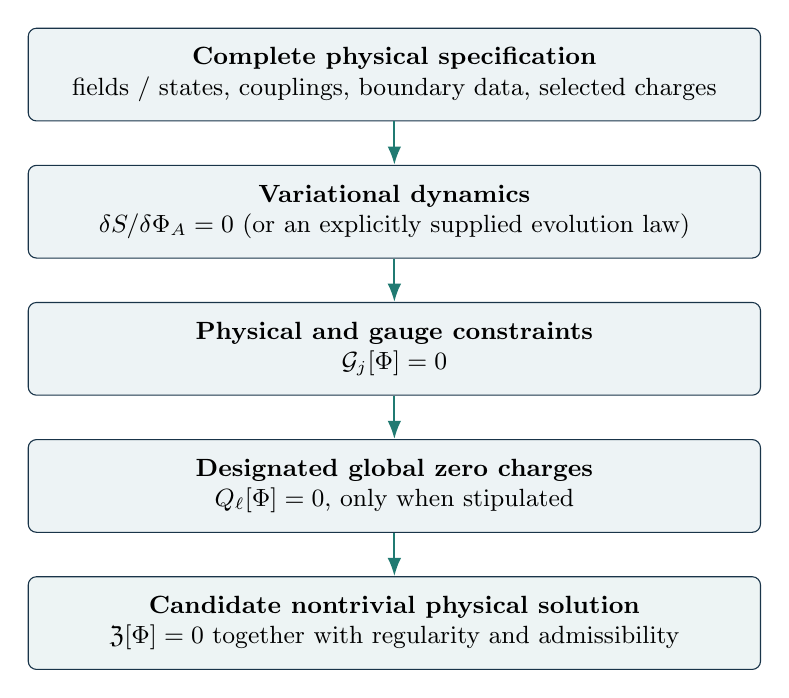
\begin{tikzpicture}[>=Latex,node distance=5.5mm, every node/.style={font=\small}, box/.style={draw=deep,rounded corners=3pt,align=center,minimum width=9.3cm,inner sep=7pt,fill=paperblue}, arrow/.style={->,thick,draw=seagreen}]
\node[box] (a) {\textbf{Complete physical specification}\\fields / states, couplings, boundary data, selected charges};
\node[box,below=of a] (b) {\textbf{Variational dynamics}\\$\delta S/\delta\Phi_A=0$ (or an explicitly supplied evolution law)};
\node[box,below=of b] (c) {\textbf{Physical and gauge constraints}\\$\cG_j[\Phi]=0$};
\node[box,below=of c] (d) {\textbf{Designated global zero charges}\\$Q_\ell[\Phi]=0$, only when stipulated};
\node[box,below=of d,fill=seagreen!8] (e) {\textbf{Candidate nontrivial physical solution}\\$\cZ[\Phi]=0$ together with regularity and admissibility};
\draw[arrow] (a)--(b);\draw[arrow] (b)--(c);\draw[arrow] (c)--(d);\draw[arrow] (d)--(e);
\end{tikzpicture}
\end{center}
The vertical layout is an \emph{audit order}, not an assertion that the equations dynamically generate their own initial data or charges.

\section{Worked example I: Poisson's equation and gravitational source--response}
\subsection{A nonzero source with an exactly zero field-equation residual}
For a sufficiently regular, localized nonnegative Newtonian mass density $\rho(\bm x)$, let $\Phi(\bm x)$ be its gravitational potential normalized by $\Phi\to0$ at spatial infinity. The Poisson equation reads
\begin{equation}\label{eq:poisson}
\boxed{\nabla^2\Phi-4\pi G\rho=0.}
\end{equation}
This is a textbook source--response balance with $\rho\neq0$ and typically $\Phi\neq0$. The unique decaying solution under standard conditions is
\begin{equation}\label{eq:Green}
\Phi(\bm x)=-G\int_{\R^3}\frac{\rho(\bm y)}{|\bm x-\bm y|}\,\dd^3y.
\end{equation}
Thus $\Phi<0$ for positive nonzero localized densities at ordinary field points. For a point mass, $\Phi=-GM/r$ away from the origin, so $\Phi+GM/r=0$ is a \emph{potential identity}, not a total-energy equation. Distributionally, $\nabla^2(-GM/r)=4\pi GM\delta^{(3)}(\bm x)$.

The source-to-field map is completely specified by the Poisson Green function; the field is \emph{not} an arbitrary negative quantity selected to enforce a desired cancellation.

\subsection{An actual negative relative interaction energy}
The Newtonian gravitational self-binding energy of a smooth isolated distribution is
\begin{align}
U_g&=\frac12\int\rho\Phi\,\dd^3x
=-\frac{G}{2}\iint\frac{\rho(\bm x)\rho(\bm y)}{|\bm x-\bm y|}\,\dd^3x\,\dd^3y,\\
&=\boxed{-\frac{1}{8\pi G}\int_{\R^3}|\nabla\Phi|^2\,\dd^3x\le0.}\label{eq:gravenergy}
\end{align}
The final identity follows by inserting equation~\eqref{eq:poisson} and integrating by parts with sufficiently fast-decaying boundary data. Its sign is an established Newtonian \emph{binding-energy} property, not proof that positive rest energy is canceled exactly.

For the explicit Gaussian source
\begin{equation}
\rho(\bm x)=\frac{M}{(2\pi)^{3/2}L^3}\exp\!\left(-\frac{|\bm x|^2}{2L^2}\right),
\end{equation}
the pair-integral gives $U_g=-GM^2/(2\sqrt\pi L)$. This is a calculable source-determined response. If one sets $Mc^2+U_g=0$ by extrapolating it into strong gravity, one exceeds the assumptions of Newtonian theory; such a putative root is \emph{not} a physically established zero-energy TUO universe.

\begin{keybox}
\textbf{Poisson lesson.} A sourced field can satisfy an exact zero residual. Gravity provides a negative \emph{relative} binding-energy contribution in a controlled limit. Neither fact alone establishes exact global energy cancellation in TUO.
\end{keybox}

\section{Worked example II: Schr\"odinger dynamics and positive-energy zero residuals}
In ordinary post-emergence quantum mechanics, the Schr\"odinger equation is
\begin{equation}\label{eq:schr}
\boxed{(\ii\hbar\partial_t-\widehat H)\psi=0.}
\end{equation}
The conventional sign is a \emph{minus}: $\ii\hbar\partial_t\psi=\widehat H\psi$. If $\widehat H\psi_E=E\psi_E$, then
\begin{equation}
\psi(t)=\psi_E\exp(-\ii Et/\hbar),\qquad
\ii\hbar\partial_t\psi-E\psi=0.
\end{equation}
For $E>0$ and $\psi\neq0$, both sides of the defining balance are nonzero while the residual vanishes. In particular, $\ave{H}=E$, \emph{not} zero.

This equation also follows from an action. For $\widehat H=-\hbar^2\nabla^2/(2m)+V(\bm x)$ with real $V$, use
\begin{equation}\label{eq:schraction}
S[\psi,\psi^*]=\int\dd t\,\dd^3x\left\{
\frac{\ii\hbar}{2}(\psi^*\partial_t\psi-\psi\partial_t\psi^*)
-\frac{\hbar^2}{2m}|\nabla\psi|^2-V|\psi|^2\right\}.
\end{equation}
Treating $\psi$ and $\psi^*$ as formally independent variables in the variation, $\delta S/\delta\psi^*=0$ yields equation~\eqref{eq:schr}. Thus Hamilton's principle, a nonzero wavefunction and positive-energy quantum evolution coexist with a zero dynamical residual.

\begin{warningbox}
\textbf{Do not infer an origin mechanism.} Equation~\eqref{eq:schr} assumes a time parameter, a Hilbert space and a Hamiltonian. It demonstrates \emph{balance during evolution}; it does not create the state, derive its Hamiltonian from Axiom~1, or license ``borrowing'' energy from the vacuum.
\end{warningbox}

\section{Worked example III: the Dirac field and its variational origin}
Use $c=\hbar=1$ and Lorentzian signature $(+,-,-,-)$ \emph{only for the present post-emergence example}. The gauge-covariant Dirac equation is
\begin{equation}\label{eq:dirac}
\boxed{(\ii\gamma^\mu D_\mu-m)\psi=0,\qquad
\{\gamma^\mu,\gamma^\nu\}=2\eta^{\mu\nu}.}
\end{equation}
A real-valued, symmetrized Dirac Lagrangian is
\begin{equation}\label{eq:DiracL}
\mathscr L_D=\frac{\ii}{2}\left[
\bar\psi\gamma^\mu D_\mu\psi-(D_\mu\bar\psi)\gamma^\mu\psi
\right]-m\bar\psi\psi.
\end{equation}
The Dirac adjoint $\bar\psi=\psi^\dagger\gamma^0$ is varied independently of $\psi$, with conjugate variation then supplying the adjoint equation. Consequently $\delta S_D/\delta\bar\psi=0$ gives equation~\eqref{eq:dirac} under the usual boundary conditions.

For a free positive-frequency rest-spinor mode $\psi(x)=u\exp(-\ii mt)$ satisfying $\gamma^0u=u$, equation~\eqref{eq:dirac} is fulfilled with $m>0$ and $u\ne0$. The mass term and time-derivative term are separately nonzero: $m u -m u=0$. The mode itself is not a finite-volume normalizable particle packet; normalizable wavepackets can be built by superposition.

The coupling to a gauge field ties the spinor equation to gauge-field equations through a current $J^{a\mu}\propto\bar\psi\gamma^\mu T^a\psi$. A self-consistent solution must solve \emph{both} matter and gauge equations, including the gauge constraints: satisfying the free Dirac equation alone is insufficient for a coupled TUO source--response configuration.

\begin{keybox}
\textbf{Dirac lesson.} A nonzero relativistic matter field and its nonzero kinetic/mass contributions can obey a zero field-equation residual. Its coupling to gauge fields is a concrete model of matter and response belonging to a \emph{single} system, not evidence for zero total physical energy.
\end{keybox}

\section{Worked example IV: Yang--Mills, genuine field self-interaction}
\subsection{Gauge geometry and complete field residual}
Let $A_\mu=A_\mu^aT^a$ be a connection for a compact Lie group, with $[T^a,T^b]=\ii f^{abc}T^c$. In conventional units $c=\hbar=1$, and with one common sign convention, the field strength can be written
\begin{equation}\label{eq:FYM}
F^a_{\mu\nu}=\partial_\mu A_\nu^a-\partial_\nu A_\mu^a
+g f^{abc}A_\mu^bA_\nu^c,
\qquad
(D_\mu X)^a=\partial_\mu X^a+g f^{abc}A_\mu^bX^c.
\end{equation}
The gauge and matter actions can be specified so that the field equation reads
\begin{equation}\label{eq:YM}
\boxed{(D_\mu F^{\mu\nu})^a-J^{a\nu}=0.}
\end{equation}
With $J^{a\nu}$ defined by the matter variation in the selected sign convention, equation~\eqref{eq:YM} becomes
\begin{equation}\label{eq:YMexp}
\underbrace{\partial_\mu F^{a\mu\nu}}_{\text{field variation}}
+\underbrace{g f^{abc}A_\mu^bF^{c\mu\nu}}_{\text{non-Abelian self-interaction}}
-\underbrace{J^{a\nu}}_{\text{matter current}}=0.
\end{equation}
The self-interaction is not optional: $F$ itself contains the quadratic term $g f^{abc} A^b A^c$. Nonzero gauge fields may therefore interact with one another even when external matter currents are absent. The $\nu=0$ component furnishes the relevant Gauss-law constraint in canonical formulations, and the equations must be understood modulo gauge redundancy \cite{YangMills1954}.

\subsection{An explicit nonlinear, non-Abelian zero-residual solution}
For a mathematically transparent \emph{non-Abelian} example choose $SU(2)$, $f^{abc}=\epsilon^{abc}$, temporal gauge $A_0^a=0$, and a spatially homogeneous ansatz
\begin{equation}\label{eq:ansatz}
\boxed{A_i^a(t)=f(t)\,\delta_i^a,\qquad a,i\in\{1,2,3\},\qquad J^{a\mu}=0.}
\end{equation}
This post-emergence Minkowski-space example has
\begin{equation}
F_{0i}^a=\dot f\,\delta_i^a,
\qquad F_{ij}^a=g f^2\epsilon^{aij}.
\end{equation}
Substitution into the Yang--Mills equation yields the nonlinear ordinary differential equation
\begin{equation}\label{eq:fode}
\boxed{\ddot f+2g^2 f^3=0.}
\end{equation}
The Gauss component vanishes for this ansatz. For smooth, nonzero initial data $f(0)=f_0$, $\dot f(0)=v_0$ the ODE has a nontrivial local (indeed global bounded) solution and the positive conserved energy density is
\begin{equation}\label{eq:ymenergy}
\boxed{\varepsilon_{\rm YM}=\frac32\left(\dot f^{\,2}+g^2f^4\right),\qquad
\frac{\dd\varepsilon_{\rm YM}}{\dd t}=3\dot f(\ddot f+2g^2 f^3)=0.}
\end{equation}
For $f_0\ne0$ or $v_0\ne0$, the physical field strengths and $\varepsilon_{\rm YM}$ are nonzero, while the \emph{entire Yang--Mills residual is zero}. The quartic term is a genuinely non-Abelian field interaction. Because the ansatz is homogeneous over $\R^3$, its \emph{total} energy is infinite; equation~\eqref{eq:ymenergy} is a valid finite \emph{density} benchmark, not a spatially localized TUO seed.

Gauge potentials themselves are gauge dependent: $A_\mu\ne0$ can sometimes describe a pure gauge with $F_{\mu\nu}=0$. In this example $F\ne0$ and the gauge-invariant local energy density is nonzero, so the nontriviality is physical rather than merely representational.

\begin{keybox}
\textbf{Yang--Mills lesson.} Nonzero field energy, nonlinear field self-interaction, and an identically vanishing \emph{full equation residual} coexist in an explicit solution. This is the strongest dynamical example here of a nontrivial zero that does not rely on a separately imposed matter source or on negative total energy.
\end{keybox}

\section{Worked example V: neutrality, Maxwell fields, and why zeros differ}
For a nonzero smooth charge distribution $\rho_q$ with $\int\rho_q\,\dd^3x=0$, Gauss's law is
\begin{equation}
\nabla\cdot\bm E-\rho_q/\varepsilon_0=0,
\qquad Q_{\rm electric}=\int\rho_q\,\dd^3x=0.
\end{equation}
An electric dipole constructed from spatially separated equal-and-opposite charge densities satisfies both relations while producing a generally nonzero electric field. Yet its classical field energy is
\begin{equation}\label{eq:Em}
\boxed{U_{\rm EM}=\frac{\varepsilon_0}{2}\int|\bm E|^2\,\dd^3x\ge0}
\end{equation}
for static electric fields under ordinary conditions. Thus neither the \emph{zero Gauss-law residual} nor the \emph{zero net electric charge} implies $U_{\rm EM}=0$.

This case is included precisely to prevent a mistaken energy inference from Axiom~2. Some physical systems have negative \emph{relative binding energy}; some fields have positive field energy; and the complete equations can equal zero in either case.

\section{The energy question: what Axiom 2 does and does not solve}
\subsection{Four mathematical zeros that must never be conflated}
\begin{table}[h]
\centering\small
\begin{tabularx}{\linewidth}{@{}p{.21\linewidth}p{.31\linewidth}Y@{}}\toprule
\textbf{Condition} & \textbf{Exact meaning} & \textbf{Does it imply zero physical energy?}\\\midrule
$\delta S=0$ & Stationary first variation for allowed perturbations & No: $S$ and $H$ may be nonzero\\
$\delta S/\delta\Phi_A=0$ & Equations of motion on shell & No: nontrivial energetic solutions are commonplace\\
$Q_{\rm electric}=0$ & Net electric charge vanishes & No: charged pairs and their fields may have positive energy\\
$E_{\rm total}=0$ & A separately \emph{defined} total-energy condition & Yes by definition for that total, but what counts as the total, and whether a nonempty solution exists, require a physical theory\\\bottomrule
\end{tabularx}
\caption{The four zeros are not logically interchangeable.}\label{tab:fourzeros}
\end{table}

If TUO further requires a genuine zero total-energy condition, the correct specialization is not to set every field-equation term to zero \emph{as energy}. Instead one must define an appropriate conserved or constrained energy functional for a chosen physical theory and test it:
\begin{equation}\label{eq:Etot}
\boxed{\cC_E[\bm\Phi]
=E_{\rm excitations}[\bm\Phi]
+E_{\rm interaction}[\bm\Phi]
+E_{\rm gravitational/boundary}[\bm\Phi]=0.}
\end{equation}
The decomposition is \emph{conditional}: individual terms need not be gauge invariant or uniquely defined in an arbitrary gravitational setting, and the notion of total energy can depend on boundaries and asymptotics. In particular, the gravitational Hamiltonian constraint and an asymptotic global energy are conceptually different quantities \cite{Wald1984}. The terms in~\eqref{eq:Etot} must not be filled in with an arbitrary compensator chosen to force cancellation.

\subsection{A source-determined compensator is a research candidate, not a consequence}
For a suitable linear response functional
\begin{equation}
\cF[F,J]=\tfrac12\ave{F,\mathcal KF}-\ave{J,F},\qquad
\delta\cF/\delta F=\mathcal KF-J=0,
\end{equation}
the on-shell functional becomes $\cF_{\on}=-\tfrac12\ave{J,\mathcal K^{-1}J}$ if the inverse and pairings exist. This illustrates why a source-determined response can contribute with an opposite sign under suitable positivity assumptions. But $\cF$ may be an action or a thermodynamic potential, \emph{not} the universe's global physical energy. In Maxwell theory, for example, the field energy remains positive; no universal ``field cancels its source energy'' theorem follows.

The scientifically decisive future TUO calculation is to exhibit a complete, properly constrained matter--field state with $E_{\rm physical}>0$ and, \emph{if imposed}, a precisely defined $\cC_E=0$, while meeting the relevant gravitational and gauge constraints. Axiom~2 says the zero need not logically mean emptiness; it does not establish that this specific energetically balanced origin state exists.

\section{Axioms 1--2 and TUO's rare-event hypothesis}
\subsection{The proposed complete configuration}
TUO separately hypothesizes an exceptionally rare event in which fundamental particle species and their antiparticles, together with the responses required by their interactions, emerge in a compact region. Axiom~2 motivates treating this as a \emph{complete coupled physical configuration}, not as matter first and an unrelated balancing field artificially attached afterward.

A correct research program must therefore specify, at the stage where ordinary physics applies, a candidate state $|\Psi\rangle$ or field configuration, its gauge-invariant observables, necessary operator constraints and boundary conditions, and any genuine total-energy requirement. For example, a quantum state with $\ave{\hat Q}=0$ need not satisfy the stronger condition $\hat Q|\Psi\rangle=0$. Similarly, zero expectation of non-Abelian color generators is insufficient by itself to establish the full local Gauss-law physical-state condition.

\subsection{The relevant end point: the hot Big Bang handoff}
The foundational paper makes \emph{no claim} that Axioms~1--2 already generate a cosmological scale factor. TUO's intended eventual handoff is a sufficiently energetic, self-consistent primordial state whose subsequent expansion and cooling can be treated using established hot-Big-Bang physics. Major obligations after the axiomatic foundation remain (i) physical origin/accounting of positive energy and (ii) persistence of an energetic aftermath despite particle--antiparticle reactions. Stability and event probability are subsidiary unless they obstruct those two obligations.

\section{Logical status, audit ledger, and falsifiable next questions}
\small
\begin{longtable}{@{}p{.10\linewidth}p{.49\linewidth}p{.33\linewidth}@{}}
\toprule
\textbf{Tag} & \textbf{Statement} & \textbf{Scientific status}\\\midrule
\endfirsthead
\toprule\textbf{Tag}&\textbf{Statement}&\textbf{Scientific status}\\\midrule\endhead
\texttt{[A1]} & An empty Euclidean $\R^3$ precedes physical emergence & Founding assumption; not derived\\
\texttt{[A2]} & Nonempty complete zero-constrained configurations may be admissible & Founding admissibility postulate\\
\texttt{[C2.1]} & Sources and physical responses can satisfy common constraints & Internal corollary; concrete examples exist\\
\texttt{[C2.2]} & Stationary action and dynamical equations allow nonzero solutions & Internal corollary; standard field theory\\
\texttt{[T2.1]} & Some zero-residual equations admit nonzero constituents & Demonstrated theorem of possibility\\
\texttt{[E-P]} & $\nabla^2\Phi-4\pi G\rho=0$ for $\rho\ne0$ & Exact standard Newtonian field equation\\
\texttt{[E-D]} & $(\ii\gamma^\mu D_\mu-m)\psi=0$ with $\psi\ne0$ & Standard relativistic matter dynamics\\
\texttt{[E-YM]} & Nontrivial $SU(2)$ fields satisfy $D_\mu F^{\mu\nu}=0$ & Constructed classical nonlinear solution\\
\texttt{[H]} & Rare simultaneous fundamental-particle/antiparticle emergence & TUO hypothesis; not derived\\
\texttt{[O-E]} & A source-determined energy balance supplies the hot-Big-Bang energy & Open; requires a physical energy functional and solution\\
\texttt{[O-A]} & The event yields a persistent hot energetic aftermath & Open; kinetics, quantum coherence and gravity matter\\
\bottomrule
\end{longtable}
\normalsize

A decisive \emph{positive} energy result would supply a fully specified nontrivial field/state and verify every relevant block of $\cZ=0$, including a genuine energy condition \emph{if demanded}. A decisive \emph{negative} result could show, for a precisely defined model class, that the requisite energy cancellation or nontrivial physical solution is mathematically impossible. Either result would advance TUO more directly than an additional arbitrary toy coupling.

\section{Foundational conclusion (preserved F001 synthesis)}
Axiom~1 stipulates an empty Euclidean three-dimensional arena, without smuggling in four-dimensional spacetime or pre-existing clocks. Axiom~2 is best expressed as the \emph{nontrivial zero-set principle}: complete physical configurations can contain nonzero matter, fields, interactions and evolution while satisfying designated vanishing dynamical residuals, gauge/physical constraints and global balances. Its source--response and variational corollaries, and the elementary nontrivial-zero theorem, belong to its internal foundation.

Poisson gravity shows a source-determined field and negative \emph{relative binding energy}; Schr\"odinger and Dirac show nonzero energetic evolution with zero field-equation residuals; Yang--Mills gives an explicit nonlinear, source-free, positive-energy field whose full equation residual is zero. Hamilton's principle organizes these examples through the vanishing of the first variation, not of the action or the energy. None proves that TUO's particular rare event occurs or that its positive matter energy is automatically canceled. They instead furnish a mathematically precise admissibility language for the next, genuinely dynamical energy-origin test.

\clearpage
\part*{Part II --- Living TUO Results: From Primordial Emergence to a Hot Cosmological Core}
\addcontentsline{toc}{part}{Part II --- Living TUO Results: Primordial Emergence to a Hot Cosmological Core}

\section{Official proof target: possibility, not a numerical fit}\label{sec:objective}
\begin{axiombox}
\textbf{Primordial Emergence --- named founding hypothesis (not Axiom 3).}
TUO proposes that an exceptionally rare, compact, complete physical configuration containing fundamental excitations and their conjugates, together with the necessary fields and constraints, becomes present in the initially empty spatial arena. \emph{Primordial Emergence} is the agreed name; ``rare'' describes its presumed occurrence, not its mathematical identity. No physical time, transition amplitude or emergence-rate law is supplied by Axiom~1 alone.
\end{axiombox}
The scientific remit of TUO ends \emph{where the conventional hot Big Bang begins}. It need not reproduce today's total cosmic energy, derive all later cosmology, or specify every intermediate scattering in order to establish conditional physical possibility. It \emph{must} show more than the existence of a single prepared hot state: the source--field configuration and the physically governed transition to a hot expanding aftermath must belong to one consistent construction.

Let $\mathscr A$ be the class of nontrivial regular post-emergence physical states obeying the applicable equations, gauge/Einstein constraints and explicitly stipulated global charges, and let $\mathscr H_{\rm hot}$ be the class of admissible radiation-rich expanding cosmological initial data. Our desired \emph{existence statement}, which is currently \textbf{unproved}, is
\begin{equation}\label{eq:goal}
\boxed{\exists\,X_0\in\mathscr A,\quad E_{\rm exc}(X_0)>0,\quad
\exists\,\tau_*>0:\quad \mathcal U_{\tau_*}(X_0)\in\mathscr H_{\rm hot}.}
\end{equation}
The evolution map $\mathcal U_\tau$ only refers to a specified \emph{post-emergence} theory; it does not postulate a clock before Axiom~1's proposed transition. The additional statement that $X_0$ actually emerges is a separate Primordial Emergence hypothesis. An open neighborhood of successful $X_0$, if found, would be stronger than one tuned data point.

\begin{figure}[htbp]\centering
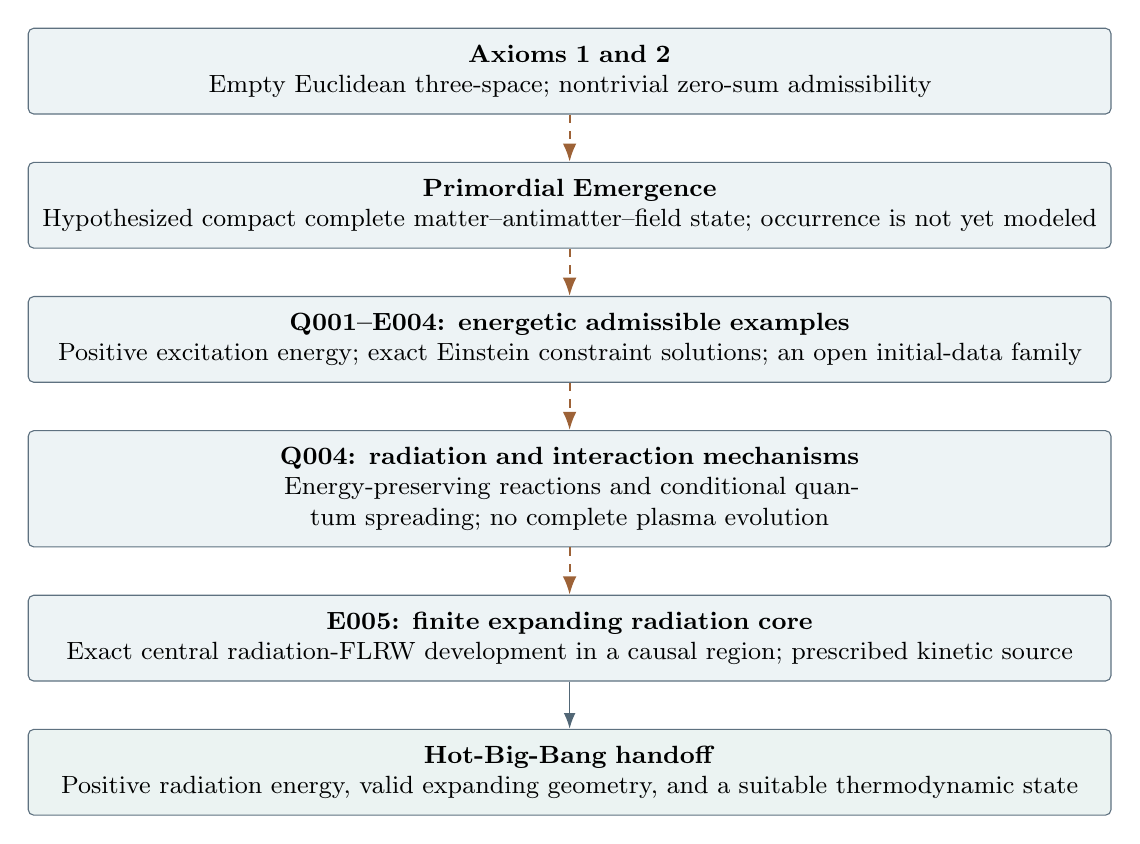
\begin{tikzpicture}[node distance=6mm, every node/.style={align=center}, >=Latex,
 block/.style={draw=deep!70,rounded corners=2pt,fill=paperblue,text width=13.4cm,inner ysep=6pt,inner xsep=5pt,font=\small},
 link/.style={->,semithick,draw=deep!75}, miss/.style={->,dashed,thick,draw=caution}]
\node[block] (a) {\textbf{Axioms 1 and 2}\\Empty Euclidean three-space; nontrivial zero-sum admissibility};
\node[block,below=of a] (b) {\textbf{Primordial Emergence}\\Hypothesized compact complete matter--antimatter--field state; occurrence is not yet modeled};
\node[block,below=of b] (c) {\textbf{Q001--E004: energetic admissible examples}\\Positive excitation energy; exact Einstein constraint solutions; an open initial-data family};
\node[block,below=of c] (d) {\textbf{Q004: radiation and interaction mechanisms}\\Energy-preserving reactions and conditional quantum spreading; no complete plasma evolution};
\node[block,below=of d] (e) {\textbf{E005: finite expanding radiation core}\\Exact central radiation-FLRW development in a causal region; prescribed kinetic source};
\node[block,below=of e,fill=seagreen!9] (f) {\textbf{Hot-Big-Bang handoff}\\Positive radiation energy, valid expanding geometry, and a suitable thermodynamic state};
\draw[miss] (a)--(b); \draw[miss] (b)--(c); \draw[miss] (c)--(d); \draw[miss] (d)--(e); \draw[link] (e)--(f);
\end{tikzpicture}
\caption{The lean TUO existence programme. Dashed arrows are \emph{not} proven evolution maps; they identify the remaining logical bridges. The solid arrow denotes the established \emph{local conditional} E005 radiation-FLRW continuation, not a completed global hot-Big-Bang origin.}\label{fig:logic}
\end{figure}

\section{Localized quantum excitation energy: what Q001 and E001--E002 establish}\label{sec:localized}
For one massless 3D Gaussian excitation with equal Cartesian position standard deviations $L$, a specified free-field wavepacket gives
\begin{equation}\label{eq:packetenergy}
\langle E\rangle=\sqrt{\frac{2}{\pi}}\frac{\hbar c}{L},\qquad
E_{\rm exc}(N,L)=N\sqrt{\frac{2}{\pi}}\frac{\hbar c}{L}.
\end{equation}
A formal $N=90$, $L=\ell_{\rm Pl}$ free-fermion count yields $71.81E_{\rm Pl}\simeq1.405\times10^{11}$\,J. The 90 label is a \emph{mode-count illustration} based on particle and antiparticle excitations of 45 Standard Model Weyl components, not a gauge-physical, interacting all-SM state and not the thermal degeneracy count $g_*=106.75$. This is the expectation energy of a \emph{prepared} nonempty state, not energy manufactured by the uncertainty principle.

E002 varies the independent input pair $(N,L)$, never tuning to a putative unique $E_{\rm universe}$. The event-duration scale $\Delta\tau$ cannot be inserted as a second additive energy resource: generic time--energy uncertainty bounds concern energy dispersion and the specific state/dynamics, whereas Eq.~\eqref{eq:packetenergy} already reflects spatial localization. Axiom~1 does not postulate ordinary pre-emergence time.

\paragraph{Thermal scales and the entropy obstruction.}
For an \emph{assumed equilibrium} relativistic gas in volume $V_*=\kappa L^3$, with constant $g_*=g_{*s}$, the standard relations are
\begin{equation}\label{eq:thermo}
\varepsilon_{\rm rad}=\frac{\pi^2}{30}g_*\frac{(k_BT)^4}{(\hbar c)^3},\qquad
\frac{s}{k_B}=\frac{2\pi^2}{45}g_{*s}\frac{(k_BT)^3}{(\hbar c)^3}.
\end{equation}
Combining $E\propto N/L$ with $E=\varepsilon V_*$ gives $T_{\rm equiv}\propto N^{1/4}/L$ and the initially assigned equilibrium entropy $S_{\rm equiv}/k_B\propto N^{3/4}$, \emph{independent of $L$ at fixed degeneracy}. Thus shrinking the packet does not automatically create the entropy of a macroscopic hot universe. The ``equivalent temperature'' is not the microscopic state temperature; actual thermalization and entropy production remain to be demonstrated. E001--E002 also show that a finite region's total positive radiation energy depends strongly on the region selected; there is no uniquely prescribed ``total energy of the Big Bang'' for a homogeneous infinite cosmology.

\section{Exact sourced gravitational energy accounting (E003)}\label{sec:e003}
We now work strictly \emph{after} the hypothesized emergence, using conventional general relativity and initially time-symmetric, spherically symmetric spatial data. Let
\begin{equation}\label{eq:e003ansatz}
\gamma_{ij}=\psi^4\delta_{ij},\qquad K_{ij}=0,\qquad
\nabla^2\psi=-\frac{2\pi G}{c^2}\widetilde\rho,\qquad \widetilde\rho=\psi^5\frac{\varepsilon}{c^2}.
\end{equation}
For an \emph{assigned conformally weighted Gaussian} $\widetilde\rho=M(2\pi L^2)^{-3/2}\exp[-r^2/(2L^2)]$, the exact positive conformal factor is
\begin{equation}\label{eq:e003psi}
\boxed{\psi(r)=1+\frac{GM}{2c^2r}\operatorname{erf}\!\left(\frac r{\sqrt2L}\right).}
\end{equation}
The Hamiltonian and momentum constraints vanish by construction; the physical matter density is nonnegative. The proper matter energy and ADM energy satisfy the exact ledger
\begin{equation}\label{eq:ledger}
\boxed{E_{\rm proper}=Mc^2+\frac{GM^2}{2\sqrt\pi L},\quad
E_{\rm binding}=-\frac{GM^2}{2\sqrt\pi L},\quad E_{\rm ADM}=Mc^2>0.}
\end{equation}
No negative field energy was freely tuned. The negative binding contribution is the difference of two well-defined energies \emph{within this specified asymptotically flat slicing}; it is not proof of a local gauge-independent gravitational energy density. In particular
\begin{equation}
\boxed{\mathcal H_{\rm GR}=0\quad\not\Rightarrow\quad E_{\rm ADM}=0.}
\end{equation}
The positive mass theorem constrains zero-ADM-energy claims for complete asymptotically flat data under standard energy conditions~\cite{CarlottoConstraints}.

If one matches only the \emph{integrated} proper energy to the Q001 $N=90$, $L=\ell_{\rm Pl}$ count, the formal ledger reads $E_{\rm proper}=71.81E_{\rm Pl}$, $E_{\rm binding}=-57.53E_{\rm Pl}$ and $E_{\rm ADM}=14.28E_{\rm Pl}$. The classical slice then has an outer spherical minimal surface; it is not a controlled, freely dispersing Planck-scale quantum calculation. The source is a classical prescribed profile, \emph{not} the expectation stress of a demonstrated gauge-invariant 90-excitation quantum state.
\begin{figure}[htbp]\centering\includegraphics[width=.85\linewidth]{E003_energy_ledger.png}
\caption{E003's exact classical energy ledger against width. The negative binding contribution is determined by the prescribed Gaussian source; a vanishing Einstein constraint does not imply zero ADM energy. The marked marginal-sphere threshold is a property of this time-symmetric spherical initial-data family.}\label{fig:e003ledger}
\end{figure}

\section{A non-fitted open positive-energy initial-data region (E004)}\label{sec:e004}
Write $\lambda=L/\ell_{\rm Pl}$, $\alpha=\sqrt{2/\pi}$, $E_{\rm proper}=N\alpha E_{\rm Pl}/\lambda$, and introduce dimensionless compactness variables
\begin{equation}\label{eq:e004xy}
 y=\frac{GE_{\rm proper}}{c^4L}=\frac{\alpha N}{\lambda^2},\qquad
 x=\frac{GM_{\rm ADM}}{c^2L},\qquad
 \boxed{y=x+\frac{x^2}{2\sqrt\pi}.}
\end{equation}
The nonnegative root $x=2y/[1+\sqrt{1+2y/\sqrt\pi}]$ determines the field response; $x$ is \emph{not} fitted independently. E004 screens a wide range for positive $E_{\rm proper}$, positive $E_{\rm ADM}$, regular gravitational constraints, no spherical minimal surface on the time-symmetric slice, and chosen conservative compactness/curvature and radiation-\emph{equivalent} density thresholds.

For the historical $N=90$ energy-normalization example, the \emph{selected screens} yield an open interval
\begin{equation}\label{eq:e004region}
\boxed{100< L/\ell_{\rm Pl}<7.33\times10^{15}.}
\end{equation}
A representative case $L=100\ell_{\rm Pl}$ has $E_{\rm proper}\simeq0.7181E_{\rm Pl}$, $x\simeq0.00717$, no initial spherical minimal sphere, and a central equivalent-radiation energy scale around $7.30\times10^{16}$ GeV. The interval is broad and involves \emph{no matching to the observed universe's total energy}. It is an \emph{initial-data admissibility} region, \emph{not} a solved quantum origin or a cosmological formation-probability region; initial ``radiation'' temperature/entropy are formal equilibrium assignments.
\begin{figure}[htbp]\centering\includegraphics[width=.88\linewidth]{E004_existence_region.png}
\caption{E004's non-fitted initial-data screening: the selected strict conditions define an open source--field existence region. The plot does \emph{not} show where the Primordial Emergence event occurs or where a hot Big Bang has already been produced.}\label{fig:e004region}
\end{figure}

\section{Annihilation and interaction-induced spreading: conditional evidence}\label{sec:interactions}
In any local energy--momentum conserving post-emergence model, matter--antimatter annihilation is not intrinsically the destruction of excitation energy. Established channels include $e^-+e^+\to2\gamma$ and inverse photon collisions, but a $2\to2$ process does \emph{not} increase the number of excitations. A real $2\to3$ channel such as $e^-+e^+\to3\gamma$ is higher-order and demands a physical amplitude and infrared-resolved photon definition. The primordial radiation and matter distributions are not inferred from net charge cancellation.

A simple exact consequence of local conservation is useful. For an isolated relativistic stress tensor with $\partial_\mu T^{\mu\nu}=0$, negligible boundary contributions and $E=\int T^{00}\dd^3x>0$, set $R_E^2=E^{-1}\int r^2T^{00}\dd^3x$. Then (in units $c=1$)
\begin{equation}\label{eq:momentid}
\frac{\dd^2R_E^2}{\dd t^2}=\frac2E\int(T^{11}+T^{22}+T^{33})\dd^3x.
\end{equation}
For a traceless source, this equals $2$ and fixes $R_E^2(t)=R_E^2(0)+\dot R_E^2(0)t+t^2$. Nevertheless, the \emph{covariance-volume} $\sqrt{\det C}$ can vary at fixed $\mathrm{tr}\,C$, and a change in shape can increase statistical volume without increasing total energy. This does not itself generate expanding spacetime.

\paragraph{Exact-unitary toy construction (Q004-U4).}
In a lattice Hamiltonian containing local coherent conversion between a neutral charged-pair-like sector and a three-photon-like sector, the \emph{expected} excitation number and spatial spread can increase while total Hamiltonian energy and norm remain constant. Under selected hopping and coupling parameters, a 1D spatial-variance ratio $6.8643/5.0898\simeq1.349$ and small 3D covariance-volume ratios $1.055$ and $1.083$ were obtained. The effect reverses if the radiation-like sector propagates more slowly. This is an existence example for interaction-enhanced spreading, \emph{not} a physical QED rate or a Heisenberg-driven cosmological-volume operator.
\begin{figure}[htbp]\centering\includegraphics[width=.82\linewidth]{Q004U4_3D_volume.png}
\caption{Q004-U4 finite 3D lattice interaction test: covariance-volume enhancement in a particular exactly unitary toy model, not a continuum or Standard Model prediction.}\label{fig:q004vol}
\end{figure}

\paragraph{Microscopic rate screen and correction.}
Q004-U5's dilute localized-packet QED calculation gives an annihilation optical depth $\tau=\sigma_{e^+e^-\to2\gamma}/(8\pi L^2)$ for an idealized Gaussian head-on pair, typically far below unity in the selected GeV examples. Q004-U6's leading-order hard-QCD screen finds larger selected interaction opportunities among many colored excitations, but soft exchange and coherence invalidate naive independent-pair counting. Neither calculation proves large-system thermalization. \textbf{Historical correction:} Q004-U2's finite-range pair-collision algorithm relocated separated particles to their midpoint, violating local energy-density continuity and spuriously reducing spatial moments. Its apparent slowdown of volume growth is \emph{withdrawn} as a physical claim; all reported results in this paper exclude that inference.

\clearpage
\section{E005 --- A finite expanding radiation core and genuine local FLRW evolution}\label{sec:e005}
This section is deliberately distinct: E005 addresses a question \emph{not} answered by particle-cloud spreading or by E004's time-symmetric initial data. \emph{Can a finite positive-energy source--field configuration include a real expanding region that obeys the radiation-era cosmological equations for a nonzero interval?} Within a specified conventional Einstein--massless-Vlasov theory, the answer is \emph{yes, conditionally}. It does \emph{not} claim that this data set is produced by TUO's original quantum emergence.

\subsection{Exact Einstein constraint construction}
Use geometrized units $G=c=1$ and a radial coordinate measured in an arbitrary length $L$. A spatial metric $\gamma_{ij}$, extrinsic curvature $K_{ij}$ and matter normal density and momentum $(\mathcal E,\mathcal J_i)$ must satisfy
\begin{equation}\label{eq:e005constraints}
\boxed{\begin{aligned}
{}^{(3)}R+K^2-K_{ij}K^{ij}&=16\pi\mathcal E,\\
D_j(K^j{}_i-\delta^j{}_iK)&=8\pi\mathcal J_i.
\end{aligned}}
\end{equation}
Introduce $\gamma_{ij}=\psi^4\delta_{ij}$ and the \emph{expanding} pure-trace extrinsic curvature $K_{ij}=-H(r)\gamma_{ij}$, with $H(r)>0$ in a central ball and $H(r)=0$ beyond a surrounding transition. For a smooth nonnegative conformal shell source $\widetilde\rho$ define
\begin{equation}\label{eq:e005source}
\Delta\psi=-2\pi\widetilde\rho,\quad
\mathcal E=\frac{\widetilde\rho}{\psi^5}+\frac{3H^2}{8\pi},\quad
\boxed{\mathcal J_r=\frac{H'}{4\pi},\quad |\mathcal J|=\frac{|H'|}{4\pi\psi^2}.}
\end{equation}
These expressions satisfy \emph{both} Einstein constraints exactly, not merely numerically. For $\widetilde\rho=\mu w(r)$ with $4\pi\int r^2w(r)\dd r=1$ supported in $2<r<4$, the solution regular at the origin and normalized at infinity is
\begin{equation}\label{eq:e005psi}
\psi(r)=1+2\pi\left[\frac1r\int_0^r s^2\widetilde\rho(s)\dd s+\int_r^\infty s\widetilde\rho(s)\dd s\right].
\end{equation}
As $\widetilde\rho$ vanishes inside $r<2$, $\psi=\psi_0$ is \emph{constant} there; outside the shell $\psi=1+\mu/(2r)$. Set $H(r)=H_0>0$ inside the core, then taper smoothly to zero entirely within the shell. The initial central data are
\begin{equation}\label{eq:e005core}
\boxed{\gamma_{ij}=\psi_0^4\delta_{ij},\quad
K_{ij}=-H_0\gamma_{ij},\quad
\mathcal E_0=\frac{3H_0^2}{8\pi},\quad \mathcal J_i=0.}
\end{equation}
They are precisely spatially flat, homogeneous and initially expanding radiation-cosmology data. The exterior is vacuum initial data with positive ADM energy; the shell contains physically nonzero matter needed for smooth matching.
\begin{figure}[htbp]\centering\includegraphics[width=.91\linewidth]{E005_radial_matter.png}
\caption{\textbf{E005 source--response construction.} Central uniform radiation density, finite annular transition, physical radial momentum flux and exterior vacuum. Unlike an unsupported sharp junction, the shell is smooth and carries actual stress.}\label{fig:e005radial}
\end{figure}

\subsection{Causal massless-particle realization}
Einstein constraints alone do not ensure that $(\mathcal E,\mathcal J)$ arise from an acceptable matter model. E005 supplies a nonnegative massless Vlasov distribution. Put $q=\mathcal J_{\hat r}/\mathcal E$, taking $q=0$ where both vanish. For $|q|<1$, define a radial matter-rest-frame boost velocity and positive rest-frame energy
\begin{equation}\label{eq:e005vlasov}
\boxed{v=\frac{3q}{2+\sqrt{4-3q^2}},\qquad e_{\rm rest}=\frac{3\mathcal E(1-v^2)}{3+v^2}>0.}
\end{equation}
Indeed, isotropic massless radiation in its local rest frame has $p=e_{\rm rest}/3$ and $q=4v/(3+v^2)$. A smooth nonnegative momentum distribution of these boosted moments realizes the required source. Since the $H'$ support lies strictly within a positive-density shell, $|\mathcal J|<\mathcal E$ holds for \emph{an open set of sufficiently small positive} $H_0$ at fixed $\mu$. Thus the complete Einstein constraints and a causal matter realization hold simultaneously, without choosing a negative-energy field independently~\cite{AndreassonVlasov}.

\subsection{The local expansion law: exactly what it means}
The central initial ball agrees, point for point, with the initial data of a spatially flat, isotropic, \emph{massless-kinetic} radiation FLRW solution. Standard local existence, domain-of-dependence uniqueness and finite signal speeds ensure that some \emph{nonzero central causal region} evolves as that FLRW model for a positive interval of proper cosmological time $\tau$. In that region
\begin{equation}\label{eq:e005FLRW}
\boxed{\frac{a(\tau)}{a_0}=\sqrt{1+2H_0\tau},\qquad
\varepsilon(\tau)=\frac{\varepsilon_0}{(1+2H_0\tau)^2},\qquad
H(\tau)=\frac{H_0}{1+2H_0\tau}.}
\end{equation}
Here $\tau$ measures time \emph{after} the initial slice, $H_0>0$ is the prescribed initial expansion, and $\varepsilon_0>0$. Equation~\eqref{eq:e005FLRW} follows from $H^2=8\pi\mathcal E/3$ and $p=\mathcal E/3$, or equivalently the Einstein--Vlasov radiation solution. For comoving points $d(\tau)=a(\tau)\Delta\chi$: their \emph{proper geometrical distance expands}. This is not merely outgoing particle trajectories, but it is \emph{decelerating radiation-era expansion}, not inflation.

\begin{figure}[htbp]\centering\includegraphics[width=.92\linewidth]{E005_local_FLRW.png}
\caption{\textbf{Dedicated E005 result.} The exact radiation-FLRW scale factor grows while its energy density decreases. The marked formal earliest shell-signal arrival is \emph{not} a guaranteed lifetime or a demonstration of prolonged global FLRW evolution.}\label{fig:e005flrw}
\end{figure}

For the representative choice $(\mu,H_0L)=(0.5,0.01)$, $\psi_0=1.082631$ and the initially homogeneous core has physical radius $\chi_c=2\psi_0^2L\simeq2.34418L$. Formally, a radial light signal first reaching the center from the transition boundary obeys
\begin{equation}\label{eq:e005null}
\tau_{\rm null}=\chi_c+\frac{H_0\chi_c^2}{2},\qquad
\frac{a(\tau_{\rm null})}{a_0}=1+H_0\chi_c\simeq1.02344.
\end{equation}
The actual justified domain is $0<\tau<\min(\tau_{\rm local},\tau_{\rm null})$ for some positive but not explicitly lower-bounded local existence time $\tau_{\rm local}$. No global lifespan or final observer-accessible cosmology is asserted by this bound.

\subsection{Non-fitted open family and the boundary of the result}
In a representative dimensionless numerical audit, the maximum shell momentum-to-energy ratio is $0.296208$ and both constraint residuals are below $7\times10^{-17}$ in the computed discretization; analytically the constraints vanish exactly. A conservative scan of $6{,}500$ $(\mu,H_0L)$ choices has $5{,}752$ passing initial causal/geometry screens. Continuity plus strict inequalities, rather than the count alone, proves an \emph{open neighborhood} of allowed parameters. The scale $L$ is free; no measured total cosmic energy is used as a fitting target.
\begin{figure}[htbp]\centering\includegraphics[width=.86\linewidth]{E005_open_region.png}
\caption{Open E005 initial-data screening in non-fitted parameters. The shaded region is \emph{not} an emergence probability density, a thermalization map or a complete Big Bang origin phase diagram.}\label{fig:e005open}
\end{figure}

\begin{warningbox}
\textbf{Exactly what E005 does NOT prove.} The radiation core, its expansion profile and the transition-shell matter were \emph{prescribed together} as Einstein--Vlasov initial data. E005 does not evolve the Q001 90-mode quantum state or E004's Gaussian source into this core; it does not compute the annihilation-made radiation distribution, entropy production, Primordial Emergence probability, or globally persistent FLRW geometry. The positive shell energy is an \emph{input}, and ADM energy is positive. The formal $\tau_{\rm null}$ is not a bound guaranteeing the solution remains globally regular that long. E005 therefore establishes \emph{post-emergence expanding-core admissibility}, not the microscopic TUO origin theorem.
\end{warningbox}


\clearpage
\section{E006 --- A reversible matter-to-radiation bridge inside the expanding core}\label{sec:e006}
\subsection{What is new: one evolving stress tensor, rather than two separate examples}
The E005 region was initially interpreted as a prescribed \emph{radiation} core. E006 makes an important constructive improvement: the \emph{same} homogeneous initial total stress can be carried instead by an equal-density, opposite-charge electron-like and positron-like massless gas, with no photons. Subsequent local \mbox{$e^-+e^+\leftrightarrow2\gamma$} conversion changes the composition of that stress while leaving its radiation equation of state unchanged. In an explicitly specified reversible kinetic relaxation model, the pair distribution, photon distribution and expanding geometry belong to a \emph{single continuous post-emergence history}. It is not a history beginning with TUO's empty Axiom-1 arena.

\begin{figure}[htbp]\centering
\includegraphics[width=.92\linewidth]{E006_bridge_overview.png}
\caption{The E006 bridge in context. The charged core is a prescribed initial post-emergence state, whereas the subsequent composition conversion is calculated within a stated reversible kinetic closure. The arrow from Primordial Emergence remains unproved.}\label{fig:e006bridge}
\end{figure}

\subsection{Balanced charged data and exact radiation moments}
Use natural units $c=\hbar=k_B=1$ in this section. On the exactly flat homogeneous E005 core initial slice, $\gamma_{ij}=\psi_0^4\delta_{ij}$ and $K_{ij}=-H_0\gamma_{ij}$. Choose equal, isotropic, massless fermion-like distributions $f_-=f_+=\exp[-p/T_0]$ and an initially empty photon distribution. They carry opposite electric charges and equal currents at the distribution level, so the net Maxwell charge/current sources vanish. The full microscopic quantum Gauss-law state remains a separate unproved construction.

Their aggregate stress is radiationlike, independent of whether the energy is carried by the charged or photon species:
\begin{equation}\label{eq:e006T}
 p_{\rm tot}=\frac13\varepsilon_{\rm tot},\qquad
 \nabla_\mu T^{\mu\nu}_{\rm tot}=0
 \Longrightarrow \dot\varepsilon_{\rm tot}+4H\varepsilon_{\rm tot}=0.
\end{equation}
Thus $\varepsilon_{\rm tot} a^4$ stays constant in the FLRW core while the separate comoving species energies exchange. A finite electron rest mass changes the exact trace-free limit by terms suppressed as $m_e^2/T^2$ for sufficiently high temperature. This is not a claim that the full Standard Model is exactly massless.

\subsection{Explicit reversible number-and-energy-conserving kinetic closure}
For two helicity/polarization degrees of freedom per species, specify common-temperature Maxwell--Boltzmann distributions
\begin{equation}\label{eq:e006dist}
 f_-=f_+=(1-x)e^{-p/T},\qquad f_\gamma=2x e^{-p/T},\qquad
 T=T_0\frac{a_0}{a},\quad 0\le x\le\frac13.
\end{equation}
Here $x$ is the photon fraction of \emph{both the total particle number and the positive radiation energy} in this particular massless classical model. The number density per species with unit fugacity is $n^0(T)=2T^3/\pi^2$. Hence $n_-=n_+=n^0(1-x)$, $n_\gamma=2n^0x$, $n_{\rm tot}=2n^0$, and $\varepsilon_{\rm tot}=12T^4/\pi^2$. The charged imbalance vanishes exactly.

Define the reversible number reaction density
\begin{equation}\label{eq:e006rate}
 R=n^0(T)^2\langle\sigma v_{\rm M}\rangle_T\big[(1-x)^2-(2x)^2\big].
\end{equation}
A conservative \emph{reactive relaxation collision operator} acts as $C_-=C_+=-(R/n^0)e^{-p/T}$ and $C_\gamma=+(2R/n^0)e^{-p/T}$ in $(\partial_\tau-Hp\partial_p)f=C$. These collision moments separately preserve net charge, total particle count for $2\leftrightarrow2$, and aggregate four-momentum. They are a \emph{defined kinetic model}, not the literal QED scattering integral: rapid re-isotropization and Maxwell--Boltzmann kinetic equilibrium are closure assumptions. The exact QED delta-function collision integral conserves the same moments but need not preserve the simple fugacity ansatz.

Taking number moments gives a nonnegative, reversible reaction equation
\begin{equation}\label{eq:e006ode}
 \boxed{\dot x=\Gamma(T)(1+x)(1-3x),\qquad
 \Gamma(T)=n^0(T)\langle\sigma v_{\rm M}\rangle_T>0.}
\end{equation}
It has stable chemical equilibrium $x_\star=1/3$. If $\Gamma(T)=\Gamma_0 a_0/a$ throughout the short interval, as in a fixed-coefficient ultrarelativistic cross-section approximation, the exact solution is
\begin{equation}\label{eq:e006solution}
 \boxed{x(\tau)=\frac{1-\exp[-4(\Gamma_0/H_0)(a/a_0-1)]}{3+\exp[-4(\Gamma_0/H_0)(a/a_0-1)]},\qquad
 \frac{a(\tau)}{a_0}=\sqrt{1+2H_0\tau}.}
\end{equation}
Thus even with no initial photons, $x(\tau)>0$ immediately for positive collision rate and approaches $1/3$ without introducing an external energy reservoir. For the stated closure, every finite $\Gamma_0>0$, $H_0>0$ defines an open range of models with such conversion, conditionally within the protected causal and regular domain. The equilibrium $1/3$ is the \emph{classical model} value, not a precise Standard Model abundance.

\begin{figure}[htbp]\centering\includegraphics[width=.90\linewidth]{E006_reactive_conversion.png}
\caption{An exact post-emergence reversible-reaction solution under the stated massless kinetic closure. The vertical marker gives E005's formal shell-signal time, \emph{not} an established lifetime for complete Einstein--Boltzmann evolution.}\label{fig:e006conversion}
\end{figure}

\subsection{The accompanying entropy consistency test}
At fixed comoving total excitation number $N_{\rm com}$, the kinetic-equilibrium closure has
\begin{equation}\label{eq:e006entropy}
 \frac{S}{k_BN_{\rm com}}=4-(1-x)\ln(1-x)-x\ln(2x),\qquad
 \frac{\dd}{\dd x}\frac{S}{k_BN_{\rm com}}=\ln\frac{1-x}{2x}>0
 \quad (0<x<1/3).
\end{equation}
The entropy per excitation grows from $4$ to $4-\ln(2/3)\simeq4.4055$, a $\simeq10.14\%$ increase in this model. This does \emph{not} imply that the original microscopic Primordial Emergence has been shown to thermalize; the result is a self-contained coarse-grained kinetic check.
\begin{figure}[htbp]\centering\includegraphics[width=.86\linewidth]{E006_energy_entropy.png}
\caption{In the chosen reversible closure, photon comoving energy increases, pair comoving energy decreases, and the kinetic entropy rises. The total comoving radiation density $\varepsilon a^4$ remains constant.}\label{fig:e006entropy}
\end{figure}

\subsection{Physical-rate plausibility and the finite-core causal interval}
The initial collision-rate coefficient can be independently benchmarked against the physical unpolarized Born $e^-e^+\to2\gamma$ cross section from the Geant4/Heitler form already tested in Q004-U5. We averaged $\sigma v_{\rm M}$ over isotropic classical relativistic momentum ensembles and retained the electron mass in the scattering kinematics. For selected initial kinetic temperatures $k_BT_0=5$--$100$ MeV, the ratio $\Gamma_0/H_0$ in the chosen idealized core is between $3.50\times10^{15}$ and $3.19\times10^{16}$. These figures are calculations for a \emph{prepared dense thermal-type gas}; they are not interactions-per-particle for TUO's compact few-excitation event. Fermi blocking, Bose stimulation, genuine kinetic thermalization, screening and weak-sector spectators are not included.

For the E005 representative initial data $H_0L=0.01$, $\psi_0=1.082631$, the homogeneous region has initial radius $\chi_c=2\psi_0^2L\simeq2.34418L$. The formal earliest signal from the transition shell corresponds to $\Delta(a/a_0)\simeq0.02344$, not to a guaranteed global regularity time. Within the exact closure, $x>0.9/3$ at that formal signal boundary if $\Gamma_0/H_0>\ln(13)/(4\times0.02344)\simeq27.36$. The physical initial-rate screen is far above this \emph{model} threshold at MeV-scale temperatures. No observed cosmic energy is fitted; the core length $L$ is determined by the chosen temperature and the fixed initial dimensionless $H_0L$.
\begin{figure}[htbp]\centering\includegraphics[width=.84\linewidth]{E006_QED_rate_screen.png}
\caption{Physical Born QED initial-rate comparison with FLRW expansion for a prescribed thermal-like electron--positron gas. It does not establish rates for the all-Standard-Model Primordial Emergence event.}\label{fig:e006qed}
\end{figure}

\begin{warningbox}
\textbf{Scope of E006.} For the first time in our post-emergence constructions, a \emph{single stated reactive kinetic model} evolves an initially photon-free, balanced charged core into a radiation-rich expanding core with conserved total stress and positive kinetic entropy production. This is a \emph{conditional composition bridge}, not a complete Primordial Emergence-to-hot-Big-Bang origin proof. The initial hot pair population, the expanding extrinsic curvature $K_{ij}$, the transition shell and its substantial positive energy are \emph{assigned} initial data. Exact microscopic QED collision kinetics and the emergence event itself are still open. Zero Einstein constraint residuals do not mean zero ADM energy. The E005 local-causality bound must not be mistaken for a demonstrated global cosmic history; E007 quantifies the small protected interval in the previously screened region.
\end{warningbox}


\section{E007 --- Where TUO hands off to the known hot Big Bang}\label{sec:e007}
This section adds an important distinction to E005--E006. A \emph{weak local handoff} is a finite region with $H>0$, $\varepsilon>0$, $p\simeq\varepsilon/3$ and a genuine FLRW evolution for some nonzero causal interval. E005--E006 provide a \emph{conditional constructive example} of that level. A \emph{strong conventional hot-Big-Bang handoff} additionally requires sufficient domain and future continuation, appropriate thermal particle content, and consistent Einstein/gauge matching. A local hot sphere does not automatically represent our cosmological radiation era.

\subsection{A direct causal-size theorem for the E005 radiation region}
The exactly flat homogeneous radiation core has a well-defined initial physical radius $R_0=2\psi_0^2L$ and initial expansion $H_0>0$. The inward \emph{comoving} travel distance of a light signal originating at its boundary during the exact FLRW development is
\begin{equation}\label{eq:e007light}
D(\tau)=c\int_0^\tau\frac{a_0}{a(s)}\,\dd s
=\frac{c}{H_0}\left[\sqrt{1+2H_0\tau}-1\right].
\end{equation}
For $u=H_0R_0/c$, equating $D(\tau_{\rm sig})=R_0$ gives
\begin{equation}\label{eq:e007bound}
\boxed{H_0\tau_{\rm sig}=u+\frac{u^2}{2},\qquad
\frac{a(\tau_{\rm sig})}{a_0}=1+u,\qquad
\frac{T(\tau_{\rm sig})}{T_0}=\frac1{1+u}.}
\end{equation}
The final relation assumes an adiabatic equilibrium plasma with approximately constant relativistic entropy degrees of freedom $g_{*s}$. In general, $g_{*s}(T)T^3a^3$ is the adiabatic invariant. Protecting the center by finite propagation until scale-factor growth $q$ requires
\begin{equation}\label{eq:e007req}
\boxed{u\equiv H_0R_0/c\ge q-1,\qquad H_0\tau(q)=\frac{q^2-1}{2}.}
\end{equation}
\emph{Interpretation:} this is a necessary condition if the central FLRW law is guaranteed \emph{only through an untouched domain of dependence}. Shell influence may or may not change the center after its possible arrival; no future collapse theorem or global failure is inferred from the bound. The positive Einstein--Vlasov local-existence time is independently unknown, so $\tau_{\rm sig}$ is not a guaranteed evolution duration.

\begin{figure}[htbp]\centering\includegraphics[width=.85\linewidth]{E007_causal_domain.png}
\caption{E007 exact radiation-FLRW signal-cone diagnostic for the representative E005 initial data. This triangular domain is a protection guarantee, not a full future solution.}\end{figure}

\subsection{What the original E005 parameter scan actually supports}
For the E005 smooth annular source $\psi_0=1+\beta\mu$ with $\beta=0.16526199625382063$. Thus $u=2(H_0L/c)(1+\beta\mu)^2$ can be calculated independently for all 6,500 scanned cases. The 5,752 satisfying E005's strict conservative matter and initial-geometry screens have
\begin{equation}
\boxed{u\le0.2211754622,\qquad a_{\rm sig}/a_0\le1.2211754622.}
\end{equation}
For the representative $(\mu,H_0L/c)=(0.5,0.01)$, $u=0.02344179756$, $a_{\rm sig}/a_0=1.02344179756$ and $H_0\tau_{\rm sig}=0.02371656$. Thus the \emph{protected} scale growth is just 2.34\%; the formal radiation-temperature decrease is 2.29\%. This is neither a statement that the core stops expanding there nor a complete survey of all possible initial data.

\begin{figure}[htbp]\centering\includegraphics[width=.88\linewidth]{E007_e005_phase_handoff.png}
\caption{Derived radius-in-initial-Hubble-units across the archived E005 phase scan. Even the largest of the previously conservatively screened examples is sub-Hubble.}\end{figure}

\subsection{A non-fitted physical stress test: cooling toward the MeV era}
At fixed $g_{*s}$, an illustrative hot-state cooling from $T_0=20$ MeV to $T_f=1$ MeV requires $q=20$, hence $u\ge19$ for the central point to remain protected from the initial shell until that temperature is reached. The corresponding FLRW interval is $H_0\tau=199.5$, compared with $0.02371656$ for the representative E005 shell-signal time. This is a \emph{test of sustained causal protection}, not a demand that TUO fit a unique cosmic energy and not a claim that the known early universe began at exactly 20 MeV.
\begin{figure}[htbp]\centering\includegraphics[width=.88\linewidth]{E007_handoff_requirement.png}
\caption{Exact size requirement $u\ge q-1$ for shielding the central region until scale growth $q$, compared with the E005 example and the screened sample maximum.}\end{figure}

There is a genuine geometric tradeoff. In a spatially flat expanding FLRW region, the signs of future outgoing and ingoing radial null expansions on spheres of areal radius $R$ follow $H+c/R$ and $H-c/R$. If $u>1$, the initial core contains \emph{anti-trapped} two-spheres beyond its Hubble radius. Such spheres are ordinary in large expanding cosmologies, but a globally regular asymptotically flat origin history must then address the associated causal/past-boundary restrictions. The classic Farhi--Guth obstacle applies to \emph{false-vacuum bubbles} under specified conditions; it should \emph{not} be treated as a proved no-go theorem for TUO's radiation source.

\subsection{The actual interface to established hot-Big-Bang physics}
A sufficient handoff must specify a post-emergence slice $\Sigma_*$ carrying $\{\gamma_{ij},K_{ij},f_A,\text{gauge fields}\}$ with
\begin{enumerate}
\item \textbf{Physical data:} positive-energy distributions, exact Einstein and relevant Gauss constraints, and no invented external energy reservoir;
\item \textbf{Expanding geometry:} $H_*>0$, radiation-like $p\simeq\varepsilon/3$, and controlled homogeneity and isotropy over an adequate \emph{cosmological} domain;
\item \textbf{Thermal identity:} actual near-equilibrium distributions and $\varepsilon=\pi^2g_*(T)(k_BT)^4/[30(\hbar c)^3]$, $s=2\pi^2g_{*s}(T)k_B(k_BT)^3/[45(\hbar c)^3]$, rather than merely an energy-density-equivalent temperature;
\item \textbf{Physical particle contents:} at a MeV-era handoff the radiation bath includes neutrinos and the baryon sector essential for BBN, while an earlier pre-baryogenesis handoff must state the subsequent matter-asymmetry premise; and
\item \textbf{Sustained continuation:} a true region-to-cosmology matching or a demonstrated self-consistent whole-core future, not only a local existence interval.
\end{enumerate}
The Particle Data Group's hot-Big-Bang account explicitly includes radiation thermodynamics, species-dependent interaction rates relative to $H$, neutrino decoupling and BBN near the MeV scale~\cite{PDGHot2025}. E006's pair--photon reaction rates address only part of item (4), and the field-content selection question is sharpened in Section~\ref{sec:s001}; E005's initial data address part of item (2).

\begin{warningbox}
\textbf{Scientific verdict of E007.} TUO now has a \emph{conditional weak local hot-radiation entry}, not a completed \emph{strong conventional hot-Big-Bang handoff}. The new causal-size bound shows why E005's positive local FLRW result cannot be extended to a standard long thermal history by assertion. This is a restricted constructive-model finding, \emph{not} a demonstration that TUO or finite-core origins are impossible. The next decisive calculation is whole-core, self-gravitating radiation/kinetic evolution and global matching, with explicit causal/anti-trapped checks. None of this supplies the missing Primordial Emergence creation mechanism from Axioms~1--2.
\end{warningbox}



\clearpage
\section{S001 --- Primordial spectrum selection and dynamical sector closure}\label{sec:s001}
\subsection{The specific particle-content problem and the proposed interpretation}
\textbf{Founding hypothesis, retained.} Primordial Emergence is proposed to be the extraordinarily rare, simultaneous, spatially overlapping realization of the \emph{full fundamental Standard-Model-compatible family}---quarks and antiquarks, leptons and antileptons, interaction/gauge fields, and the Higgs sector---as part of a single physically consistent source--field configuration. This is a hypothesis of the origin theory, \emph{not} a quantum-state construction established by Axioms~1--2. At the relevant high-energy stage, underlying gauge fields and representations are more precise than assigning every familiar low-temperature massive particle an independent initial occupation. The often-used Q001 $N=90$ fermionic packet is \emph{not} a complete gauge-constrained realization of this full family.

\textbf{New hypothesis (S001).} After the event, particle production, annihilation, scattering, composite formation and symmetry changes occur within an \emph{already specified field algebra and interaction theory}. Later particles inherit the \emph{allowed field content and processes}, not the literal identity or constituents of whichever particles collided to create them. Thus an apparently exotic \emph{post-emergence particle} may be an unusual composite, resonance, or excitation permitted by that fixed theory; it need not be a newly born fundamental field. The term \emph{primordial spectrum selection} denotes this putative selection of an underlying field sector, and \emph{dynamical closure} denotes its subsequent invariance under time evolution. Neither has been derived from Axiom~2.

In established quantum field theory, particle species are associated with quantized fields and representations, and interactions can change the numbers of excitations while retaining the action's chosen field content~\cite{CERNStandardModel,PDGHot2025}. For example, sufficiently energetic $e^-e^+$ collisions can produce $\mu^-\mu^+$ even without muons in the incoming state. The muon field was already present in the theory; it was not generated as a novel fundamental field by that collision. Electroweak symmetry breaking and QCD confinement can change the convenient effective particle description without necessarily changing underlying fundamental fields.

\begin{keybox}
\textbf{S001 working proposition (not a third axiom).} There exists at least one fully gauge-consistent post-Primordial-Emergence sector $\mathscr S_\star$, containing the Standard-Model-compatible field family and appropriate gravity, such that its physical states and Hamiltonian evolution form a dynamically closed domain throughout the TUO-to-hot-Big-Bang handoff. New quanta and composites may be produced without unbounded creation of new fundamental field \emph{types}. Whether the original emergence selects this sector is an \emph{open selection problem}. We do not demand that this be the unique possible universe.
\end{keybox}

\subsection{Exact mathematical criterion: what ``freezing'' would actually mean}
For a \emph{specified post-emergence} regularized quantum theory, let $\mathcal H_{\mathrm{phys}}$ satisfy Gauss constraints, and let $P_\star$ be an orthogonal projector onto the candidate physical sector $\mathcal H_\star=P_\star\mathcal H_{\mathrm{phys}}$. Set $Q_\star=I-P_\star$. For a time-independent self-adjoint Hamiltonian $H$ with an invariant domain, sufficient exact closure conditions are
\begin{equation}\label{eq:s001closure}
P_\star D(H)\subseteq D(H),\qquad [P_\star,H]=0
\quad\Longrightarrow\quad
Q_\star e^{-iHt/\hbar}P_\star=0\quad (t\in\mathbb R).
\end{equation}
In a finite-dimensional cutoff model with $H=H^\dagger$, the off-diagonal block condition $Q_\star H P_\star=0$ is equivalent to both off-diagonal blocks vanishing (the adjoint gives $P_\star H Q_\star=0$), so it establishes the same result. This is a \emph{conditional invariant-subspace lemma} about the chosen $H$, not proof that Primordial Emergence selects $H$ or $P_\star$. Gauge-physical projection and symmetry/charge selection must be implemented at the level of the actual field theory.

\textbf{Two different notions of closure must be distinguished.} A field list fixed by definition is \emph{kinematic field-content closure} of the specified effective QFT; it can include interactions that produce additional included species. A strict exclusion of a sector of an \emph{enlarged} theory is \emph{dynamical closure} and requires the invariant-subspace condition. Neither the absence of exotic particles initially nor a mere energy threshold proves the latter.

\subsection{Illustrative solvable counterexample: initially absent exotics need not stay absent}
Consider two orthonormal states $|s\rangle$ (an allowed-sector state) and $|x\rangle$ (a hypothetical exotic-sector state) with the time-independent Hermitian Hamiltonian
\begin{equation}\label{eq:s001toy}
H=\begin{pmatrix}0&g\\g&\Delta\end{pmatrix},\qquad
|\psi(0)\rangle=|s\rangle,\qquad
P_x(t)=\frac{4g^2}{\Delta^2+4g^2}
\sin^2\!\left(\frac{\sqrt{\Delta^2+4g^2}\,t}{2\hbar}\right).
\end{equation}
$P_x(0)=0$ in every case. Yet $g\ne0$ allows a nonzero later exotic-sector occupation; the maximum $4g^2/(\Delta^2+4g^2)$ is suppressed for weak mixing $|g|\ll|\Delta|$ but is exactly zero for all times only when $g=0$ (in this example). The model is an exact two-level quantum calculation, \emph{not} a Standard Model scattering prediction, exotic relic abundance, or an origin mechanism.
\begin{figure}[htbp]\centering
\includegraphics[width=.91\linewidth]{S001_sector_leakage.png}
\caption{\textbf{S001 reproducible invariant-sector test.} Exact $P_x(t)$ from Eq.~\eqref{eq:s001toy}, with $\Delta=1$ in arbitrary energy units and $g/\Delta=0,0.05,0.25,1$. A vanishing initial exotic population does not imply exact long-term exclusion when sector mixing is present. Reproduced independently by matrix exponentiation in \texttt{verification/S001\_sector\_leakage\_verify.py}.}\label{fig:s001leak}
\end{figure}

\subsection{What counts as exotic, and why no absolute ban is established}
\begin{table}[htbp]\centering\small
\begin{tabularx}{\linewidth}{@{}p{.27\linewidth}YY@{}}\toprule
\textbf{Case} & \textbf{Post-emergence possibility} & \textbf{Scientific implication}\\\midrule
Unusual hadron, bound state, resonance & May be produced using existing Standard Model fields & Exotic \emph{appearance}, not a new fundamental field type\\
Additional heavy field \emph{not} in $\mathscr S_\star$ & Not produced by a theory whose field algebra excludes it & Closure is true \emph{conditional on} the selected complete field content\\
Additional field included in an enlarged theory, with portal coupling & Can be produced when dynamics permits, even if absent initially & Initial zero population does not imply exact exclusion\\
Heavy field with suppressed rates or decays & Can become negligibly populated & Effective decoupling/depletion, not exact invariant-sector closure\\
\bottomrule\end{tabularx}
\caption{Spectrum selection is not the same thing as prohibiting all unfamiliar particles.}\label{tab:s001cases}
\end{table}

For instance, a gauge-singlet scalar $X$ in an \emph{enlarged} field theory could have a Higgs portal $\mathcal L_{\mathrm{int}}=-\lambda_X X^2 H^\dagger H/2$; a parity $X\mapsto-X$ forbids some odd-$X$ processes but \emph{does not} generically forbid pair production $XX$. Gauge anomaly cancellation, positivity, conserved charges and regularity constrain admissible theories, but Standard Model anomaly consistency alone is not a uniqueness proof against vector-like additions~\cite{PDGVectorlike}. Indeed, our measured neutrino masses already require physics beyond the strictly minimal massless-neutrino formulation~\cite{CERNBSM}. Axiom~2's nontrivial-zero condition by itself neither selects the Standard Model nor requires an infinite tower of exotic species.

\subsection{Consequences for the early hot-plasma handoff}
TUO may therefore investigate a \emph{Standard-Model-compatible closed branch} without asserting that all logically possible exotic sectors disappear from nature. The relevant handoff data must specify (i) the physical field and gauge representations, (ii) a gauge-constrained populated state, (iii) permitted collision and conversion channels, and (iv) any extra species' energy density and interaction/decay rates. If initial exotic excitations were present in a larger selected theory, annihilation or decay may deplete them; this \emph{does not remove their fundamental fields}. Alternatively, a branch with no beyond-Standard-Model fields may be chosen as an existence candidate, but the origin's selection of that branch remains unproved.

The founding simultaneous matter--antimatter emergence also does not automatically produce a surviving baryon asymmetry. Exactly symmetric baryon number under $B$-conserving interactions remains symmetric. TUO can consistently aim for a \emph{pre-baryogenesis} hot handoff, provided later appropriate asymmetry-generating physics is separately specified and compatible with the handoff history.

\begin{warningbox}
\textbf{S001 verdict and unresolved obligation.} Post-emergence particle production can operate without adding a fresh fundamental field type whenever the underlying QFT sector is fixed. An exact invariant-sector criterion and an independently verified toy counterexample now make ``spectrum freezing'' mathematically precise. \emph{We have not derived a freezing transition, uniquely selected the Standard Model, excluded every exotic field, or constructed a full gauge-physical Primordial Emergence state.} S001 is a conditional sector-selection proposal that sharpens the physical particle-content gate of E007; it is not a third founding axiom.
\end{warningbox}

\clearpage

\clearpage
\section{C001 --- Constants as parameters of a permissible Primordial Emergence branch}\label{sec:c001}
\subsection{The new question and a strict distinction between possibility and selection}
TUO's S001 proposal concerns the field content selected by Primordial Emergence. The associated and more general question is whether the same event also selects a physically complete set of \emph{couplings, masses, mixing parameters and vacuum data}. We investigate this as \textbf{C001: Primordial Parameter-Sector Admissibility and Selection}, a \emph{candidate conditional proposition, not an extra axiom}. The existence of a consistent configuration is logically weaker than the occurrence of an event and weaker still than the determination of our measured constants.

\textbf{Clarified founding interpretation (C002).} TUO does \emph{not} propose that its two axioms uniquely compute the numerical constants observed in our universe. Rather, Primordial Emergence is hypothesized to realize \emph{contingently} one complete permissible sector---field content, action, independent physical constants and initial state---localized in the initially empty spatial arena. This is a statement of TUO's proposed chance-based origin, \emph{not} a demonstrated stochastic process or a rule for the numerical probability of each sector. Section~\ref{sec:c002} makes this distinction explicit.

Let $\mathscr F$ denote an allowed field/representation family, $\theta$ a collection of independent \emph{physical} theory parameters at an explicitly chosen reference renormalization scale $\mu_0$, and $S_{\mathscr F,\theta}[\Phi;\mu_0]$ its action. The dimensionless physical parameter space is a quotient by field redefinitions, gauge redundancies and changes of renormalization convention; not every written Lagrangian coefficient is an independent observable. Generalizing the typed Axiom-2 operator without changing the axiom, write
\begin{equation}\label{eq:c001family}
\mathfrak Z_{\mathscr F,\theta}[\Phi]
=\left(\frac{\delta S_{\mathscr F,\theta}}{\delta\Phi_A},\;\mathcal G_j[\Phi;\theta],\;Q_k[\Phi;\theta]\right)^\mathsf T=0.
\end{equation}
The parameter vector $\theta$ \emph{labels} the dynamical equations. It is not automatically varied in their Euler--Lagrange equations. Declaring $\delta S/\delta\theta=0$ would promote parameters to additional dynamical or auxiliary variables and would require new physical equations and boundary conditions: it is \emph{not} a consequence of Axiom~2.

\begin{definition}[A permitted parameter branch]\label{def:c001}
For specified post-emergence dynamics, let $\mathcal P(\mathscr F,\theta)$ be the set of gauge-physical, finite-energy, regular initial states whose complete constraints vanish. The \emph{admissible parameter locus} is
\[
\Theta_{\rm adm}(\mathscr F)=\{\theta:\mathcal P(\mathscr F,\theta)\ne\varnothing\}.
\]
For a specified non-fitted physical hot-Big-Bang handoff class $\mathcal H_{\rm hot}$, the stronger \emph{handoff-viable locus} is
\begin{equation}\label{eq:c001viable}
\Theta_{\rm hot}(\mathscr F)=\{\theta\in\Theta_{\rm adm}(\mathscr F):\exists\,\Phi_0\in\mathcal P(\mathscr F,\theta),\ \exists\,t_*>0:\mathcal U_{\mathscr F,\theta}(t_*)\Phi_0\in\mathcal H_{\rm hot}\}.
\end{equation}
The time variable here describes a \emph{post-emergence} evolution; Axiom~1 supplies no pre-emergence physical clock.
\end{definition}

This distinguishes three claims: \emph{parameter permission} $\theta\in\Theta_{\rm adm}$; \emph{hot-universe possibility} $\theta\in\Theta_{\rm hot}$; and \emph{event selection} of $\theta_\star$ by a physical Primordial Emergence process. The third has not been derived. No probability of any parameter value can be inferred without a defined event measure or selection dynamics; for continuous measures an exact point typically has probability zero, so physically meaningful statements involve intervals, neighborhoods or conditional distributions.

\subsection{A precise non-selection result following from the Yang--Mills example}
\begin{proposition}[Axiom-2 zero residuals do not select unique couplings]\label{prop:c001nonunique}
There exist continuum-many distinct positive values of a dimensionless field coupling $g$ for which the associated post-emergence field equations admit nontrivial positive-energy-\emph{density} solutions satisfying all their relevant local source-free gauge constraints. Consequently, the condition $\mathfrak Z_{\theta}[\Phi]=0$ together with nontriviality and positivity does \emph{not}, by itself, uniquely determine the coupling parameter.
\end{proposition}
\begin{proof}
Take the original Foundational $SU(2)$ homogeneous Yang--Mills ansatz $A_i^a=f(t)\delta_i^a$, with $A_0^a=0$, in $3+1$ post-emergence Minkowski geometry and $\hbar=c=1$. Gauss's law vanishes identically. The spatial gauge equations and conserved positive energy density reduce to
\begin{equation}\label{eq:c001su2}
\ddot f+2g^2 f^3=0,\qquad
\varepsilon_g=\frac32(\dot f^{\,2}+g^2f^4)>0
\quad\text{for nonzero initial data}.
\end{equation}
For every $g>0$ and every amplitude $A>0$, choose $f(0)=A$, $\dot f(0)=0$. An explicit global solution is
\[
f_g(t)=A\,\operatorname{cn}\!\left(\sqrt2\,gAt\,\middle|\,\frac12\right),
\qquad\varepsilon_g=\frac32g^2A^4>0,
\]
where $\operatorname{cn}$ is the Jacobi elliptic cosine. The identity $\operatorname{cn}''(u\,|\,1/2)=-\operatorname{cn}^3(u\,|\,1/2)$ verifies the ODE exactly; the conserved positive energy density bounds the solution. The homogeneous configuration on noncompact $\R^3$ has infinite integrated energy; this example is a coupling-nonselection counterexample, \emph{not} a finite-energy Primordial Emergence candidate. Thus all such $g$ yield legitimate nontrivial zero-residual field configurations. No single $g$ is selected by zero residuals or positivity alone. The example is \emph{post-emergence Yang--Mills physics}; it is not a construction of Primordial Emergence.
\end{proof}
\begin{figure}[htbp]\centering
\includegraphics[width=.94\linewidth]{C001_su2_coupling_family.png}
\caption{\textbf{C001 exact non-selection example.} Three distinct arbitrary couplings $g>0$ each admit a different, smooth nontrivial $SU(2)$ Yang--Mills solution with exact zero equations of motion and positive conserved energy density. The Jacobi-function solutions were separately checked against high-accuracy numerical ODE integration in \texttt{verification/C001\_constants\_verify.py}. This graph demonstrates \emph{permission without unique selection}, not a distribution of universe probabilities.}\label{fig:c001family}
\end{figure}

\subsection{Which constants are physically consequential? Dimensionless parameters and scale}
\emph{Dimensionful} constants such as $c$, $\hbar$ and a mass parameter encode physical structures but their bare numerical values depend on the choice of units. The modern SI even \emph{defines} units by fixed values of specified constants~\cite{BIPMUnits}. It is therefore more meaningful to ask TUO to constrain physically invariant dimensionless ratios and relations~\cite{UzanConstants}.

An illustrative nonredundant physical parameter description may contain, at a specified renormalization scale and scheme:
\begin{equation}\label{eq:c001theta}
\theta_{\rm phys}(\mu_0)=\big(\alpha_1,\alpha_2,\alpha_3,\lambda_H,
\{y_f\},\theta_{\rm CKM},\delta_{\rm CKM},\theta_{\rm QCD},\
\theta_{\nu},\ \mu_H^2/\mu_0^2,\ G\mu_0^2/(\hbar c^5)\big)_{\rm independent}.
\end{equation}
Here $\mu_0$ is an \emph{energy} reference, hence the displayed gravity ratio $G\mu_0^2/(\hbar c^5)$ is dimensionless; neutrino terms $\theta_\nu$ are theory-dependent, and the Higgs term and choice of mass normalization require consistent conventions. An alternative equally meaningful observable basis uses $\alpha=e^2/(4\pi\epsilon_0\hbar c)$, mass ratios $m_e/m_p$, $m_\nu/m_e$, the measured CKM/PMNS parameters, $\alpha_G(m)=Gm^2/(\hbar c)$, and a vacuum-energy density ratio $\rho_\Lambda/\mu_0^4$ in natural units. The cosmological constant and neutrino mass operators depend on the complete gravity/matter model. These lists are illustrative coordinates, \emph{not} extra independent parameters to count twice; parameters related by running or field redefinition must not be double-counted. The Particle Data Group lists the independent inputs of the electroweak Standard Model and stresses their renormalization conventions~\cite{PDGEW2025}.

\textbf{Running is not a fresh selection at every energy.} Once a coupling is selected at $\mu_0$, established renormalization-group equations relate its values at other scales. For example, at leading order in QCD and within one fixed-flavour perturbative regime,
\begin{equation}\label{eq:c001rg}
\frac{\dd\alpha_s}{\dd\ln\mu}=-\frac{\beta_0}{2\pi}\alpha_s^2,
\quad\alpha_s(\mu)=\frac{\alpha_s(\mu_0)}{1+\frac{\beta_0\alpha_s(\mu_0)}{2\pi}\ln(\mu/\mu_0)},\quad\beta_0=11-\frac23n_f.
\end{equation}
The corresponding RG-invariant scale is $\Lambda_{\rm QCD}/\mu_0=\exp[-2\pi/(\beta_0\alpha_s(\mu_0))]$ in this one-loop convention. A dimensionless ultraviolet coupling can thereby generate a dimensionful infrared scale through \emph{dimensional transmutation}; it does not mean Axiom~2 derived the coupling. Exact multi-loop and heavy-flavour threshold matching are omitted from this controlled illustration~\cite{PDGQCD2025}.
\begin{figure}[htbp]\centering
\includegraphics[width=.94\linewidth]{C001_rg_trajectories.png}
\caption{\textbf{C001 illustrative renormalization-group trajectories.} A family of different $\alpha_s(\mu_0)$ inputs induces different running curves through the same one-loop QCD equation with fixed $n_f=5$. Three inputs are illustrative and deliberately \emph{not fitted} to measured values. Verified by reconstructing the identical RG-invariant $\Lambda/\mu_0$ at every plotted scale.}\label{fig:c001rg}
\end{figure}

\subsection{Fixed post-emergence constants versus physically stabilized moduli}
There are two conceptually different ways a branch could possess stable constants. First, a fixed post-emergence action may simply \emph{contain} numerical coupling parameters $\theta_\star$; subsequent particle creation does not change those bare theory labels, although measured effective couplings vary with the renormalization scale. This is internal consistency of an assumed theory, not an explanation of why those parameters were selected. Second, effective couplings could depend on dynamical fields (moduli) which later settle to stable values. Then a physical \emph{stabilization mechanism} would be needed to justify their persistence.

For an illustrative scalar modulus $\varphi$ in an already existing expanding Lorentzian region, consider
\[
\mathcal L_{\varphi,F}=-\tfrac12(\nabla\varphi)^2-V(\varphi)-\tfrac14 Z(\varphi)F_{\mu\nu}F^{\mu\nu},
\qquad g_{\rm eff}^{-2}(\varphi)=Z(\varphi)>0.
\]
If gauge-field backreaction is negligible and $\varphi$ is homogeneous, a sufficiently smooth effective potential with a stable minimum $V'(\varphi_\star)=0$, $V''(\varphi_\star)>0$ yields
\begin{equation}\label{eq:c001modulus}
\ddot\varphi+3H\dot\varphi+V'(\varphi)=0,\quad
\frac{\dd}{\dd t}\left(\tfrac12\dot\varphi^2+V(\varphi)\right)=-3H\dot\varphi^2\le0\quad(H>0).
\end{equation}
Thus expansion damps the modulus's mechanical energy and \emph{can} help it settle near a stable minimum, with asymptotic convergence requiring additional conditions on the potential and global dynamics. This is a conventional conditional field-theory example, not a derivation of $V$, of $\varphi_\star$, or of the selected coupling value from TUO. Moduli stabilization may be difficult and cannot be declared for every constant merely because the Hamiltonian constraint vanishes. Once stabilized, fixed underlying parameters can still produce the normal renormalization-group running in Eq.~\eqref{eq:c001rg}.

\subsection{Contingent selection: what TUO hypothesizes and what remains to prove}
Suppose a particular Primordial Emergence branch realizes $(\mathscr F_\star,\theta_\star,\Phi_{0\star})$. S001's fixed-field hypothesis can be extended consistently by requiring the subsequent dynamics to use one and the same $S_{\mathscr F_\star,\theta_\star}$, and renormalization-group evolution derived from it:
\begin{equation}\label{eq:c001selection}
\underbrace{\big(\mathscr F_\star,\theta_\star,\Phi_{0\star}\big)}_{\text{postulated Primordial Emergence output}}
\xrightarrow{\ \mathcal U_{\mathscr F_\star,\theta_\star}\ }
\underbrace{\Phi_{\rm hot}}_{\text{candidate hot-Big-Bang handoff}}.
\end{equation}
In the clarified TUO proposal, the realization of $\theta_\star$ is \emph{contingent}, not uniquely computable from Axioms~1--2. This is a founding hypothesis about a chance-based Primordial Emergence, not a conclusion proved by the zero-residual equations. A physically specified stochastic rule or measure would be needed to calculate the frequency or relative likelihood of branch occurrence, and a dynamical origin law would be needed to derive how the selection physically happens; neither is supplied by the axioms. \emph{Neither is a prerequisite for stating the lean conditional existence problem}, but neither may be claimed as a solved mechanism. Anomaly cancellation, unitarity, positivity, well-posedness and stability constrain allowed $\theta$ without uniquely fixing all Standard Model masses, couplings and mixing angles. The immediate research programme is to determine whether $\Theta_{\rm hot}$ is nonempty, and ideally contains a robust family, without fitting numerical cosmic energy. An open set cannot be assumed when quantization or topological restrictions generate discrete or lower-dimensional parameter loci.

\begin{table}[htbp]\centering\small
\begin{tabularx}{\linewidth}{@{}p{.25\linewidth}YY@{}}\toprule
\textbf{C001 logical level}&\textbf{Mathematical question}&\textbf{Current scientific status}\\\midrule
Permissibility & Does some $\Phi$ solve the constraints for a given $\theta$? & Established in explicit post-emergence examples; many couplings allowed\\
Handoff compatibility & Does the \emph{same} $\theta$ support one evolving hot-cosmology branch? & E005--E007 partial, globally open\\
Contingent selection & Does a hypothesized emergence realize one jointly specified sector? & TUO founding hypothesis; no event mechanism or measure derived\\
Numerical prediction & Can one derive or statistically weight observed dimensionless ratios? & Not derived; not required for the lean existence target\\
\bottomrule\end{tabularx}
\caption{Axiom-2 permissibility, a physical branch, selection, and numerical explanation are distinct proof obligations.}\label{tab:c001levels}
\end{table}

\subsection{Comparison with related parameter-selection programmes and the TUO claim}
The idea of multiple consistent theories or vacuum branches with differing effective constants is \emph{not unique to TUO}. String flux-compactification landscapes explore many vacua and effective parameters~\cite{FluxLandscape}; asymptotic-safety programmes constrain couplings through renormalization-group critical surfaces~\cite{AsymSafe2024}; anthropic bounds constrain some parameter values conditionally on cosmic structure~\cite{Weinberg1987}. TUO's possible distinguishing \emph{research organization} is to combine a hypothesized single local Primordial Emergence, physically complete field/parameter-sector selection, and a constructive hot-Big-Bang handoff, without requiring a precision fit to present cosmic total energy. It would be premature to claim this as an established advantage over those proposals until TUO supplies an actual selection law or a new quantitative constraint on dimensionless parameters.

\begin{warningbox}
\textbf{C001 scientifically defensible verdict.} There is a rigorous distinction between (i) physical theories that \emph{permit} internally consistent nonzero configurations, (ii) an event that \emph{selects} one such theory and its independent dimensionless parameters, and (iii) an explanation of the particular constants observed here. The first is possible in continuum-many coupling branches, as proved by the exact Yang--Mills family. The second is now explicitly \emph{postulated as contingent Primordial Emergence}, not as a unique numerical deduction; the axioms do not supply the emergence law or any branch probabilities. The third is not among TUO's minimal existence targets. C001/C002 extend S001 conditionally and do not constitute a third axiom, a demonstrated stochastic dynamics or a prediction of all observed constants. TUO remains a lean existence programme: seek one non-fitted, physically consistent Standard-Model-compatible branch and genuine evolution to the hot Big Bang.
\end{warningbox}


\clearpage
\section{C002 --- Contingent Primordial Selection of a Complete Physical Branch}\label{sec:c002}
\subsection{The clarified founding hypothesis: chance, not a unique constants theorem}
TUO's founding interpretation is now explicit: Primordial Emergence is hypothesized to \emph{contingently} realize one complete physical configuration, including its field content and its dimensionless coupling and mass parameters. The event is not claimed to be inevitable or to select the only configuration logically compatible with Axioms~1--2. Different physically consistent emergent branches could in principle carry different constants; only the realized branch governs the subsequent physical history. ``Contingent'' means that the particular outcome is not deduced uniquely from the admissibility axioms, \emph{not} that a uniform distribution, Poisson process, quantum amplitude or independent random choice for every parameter has been derived.

This statement is \emph{part of the Primordial Emergence research hypothesis}, not a third axiom. Axiom~1 supplies an initially empty Euclidean spatial arena but no pre-existing physical time; thus colloquial descriptions such as a ``random event at one time and place'' must be read as a localized emerging configuration and the beginning of its \emph{post-emergence} temporal dynamics, without inserting a prior clock or vacuum fluctuations. Axiom~2 is a permissibility principle for nontrivial complete constraints, not a physical lottery mechanism. The hypothesis is therefore logically clear but not yet a demonstrated theory of the event's occurrence.

\begin{definition}[Complete branch and hot-handoff subset]\label{def:c002branch}
Let $b=(\mathscr F,\theta,S_{\mathscr F,\theta},\Phi_0)$ denote a physically distinct complete \emph{post-emergence} branch, modulo gauge transformations, field redefinitions and equivalent parameter conventions. It must include (i) a gauge/quantum-consistent full field family and governing action, (ii) an internally consistent set of independent physical parameters, including the relevant dimensionless quantities, and (iii) a nontrivial, constraint-compatible initial source--field configuration. Write
\begin{align}\label{eq:c002sets}
\mathscr B_{\rm adm}&=\{b:\ \Phi_0\ne0,\ \mathfrak Z_b[\Phi_0]=0,\ \mathrm{Consistent}(b)\},\\
\mathscr B_{\rm hot}&=\{b\in\mathscr B_{\rm adm}:\ \exists\,\tau_*>0,\ \mathcal U_b(\tau_*)\Phi_0\in\mathscr H_{\rm hot}\}.
\end{align}
Here $\mathrm{Consistent}(b)$ abbreviates the regularity, gauge/quantum, positivity and other applicable physical consistency requirements specified above.
The time parameter $\tau$ pertains only to the branch's \emph{post-emergence} evolution. The sets are a precise \emph{target definition}; their nonemptiness in the complete TUO origin-to-handoff theory has not yet been proved.
\end{definition}

The contingent-selection premise is then written schematically as
\begin{equation}\label{eq:c002selection}
\boxed{\mathscr B_{\rm adm}\ni b_\star=(\mathscr F_\star,\theta_\star,S_\star,\Phi_{0\star})
\quad\xrightarrow{\ \text{post-emergence dynamics }\mathcal U_{b_\star}\ }\quad
\Phi_\star(\tau),}
\end{equation}
where the \emph{realization} of $b_\star$ is hypothesized, and its evolution is to be tested. Selection of the branch is a \emph{joint} physical event, not separate unconstrained draws of $\alpha$, Yukawa ratios, gauge groups and quantum states; their interrelations must satisfy consistency, renormalization and handoff requirements.

\subsection{Why admissibility does not assign probabilities: a short exact result}
\begin{proposition}[No probability law from a list of allowed branches]\label{prop:c002measures}
Knowing the nonempty admissible set $\mathscr B_{\rm adm}$ and the subset $\mathscr B_{\rm hot}$ does not determine the probability that Primordial Emergence selects a hot-handoff-compatible branch.
\end{proposition}
\begin{proof}
It suffices to take a purely illustrative finite set of three distinct permissible branches $\mathscr B_{\rm adm}=\{b_A,b_B,b_C\}$ with $\mathscr B_{\rm hot}=\{b_B\}$. For any $q\in[0,1]$, assign a normalized nonnegative measure by
\begin{equation}\label{eq:c002finite}
\mu_q(\{b_A\})=\frac{1-q}{2},\qquad
\mu_q(\{b_B\})=q,\qquad
\mu_q(\{b_C\})=\frac{1-q}{2},\qquad
\mu_q(\mathscr B_{\rm hot})=q.
\end{equation}
Every $\mu_q$ has exactly the same admissible and hot-subset membership, while their success probabilities can take any value from zero to one. Hence membership constraints alone cannot fix an occurrence probability. This is an elementary measure-theoretic counterexample, \emph{not} a prediction that TUO has three branches or any of the displayed probabilities.
\end{proof}

If a probability space $(\mathscr B_{\rm adm},\Sigma,\mu)$ is supplied by future physical theory, the stochastic chance of a hot-compatible outcome is $\mu(\mathscr B_{\rm hot})$, provided the subset is measurable. A nonempty $\mathscr B_{\rm hot}$ is the required \emph{conditional existence} target, but does \emph{not} itself prove $\mu(\mathscr B_{\rm hot})>0$. Conversely, for a continuous parameter measure a particular exact $\theta_\star$ can have zero point probability while every sufficiently small physically admissible neighborhood has nonzero probability. Nonempty, positive support and positive integrated event probability are logically distinct. No branch measure or event rate has been calculated in TUO.

\begin{figure}[htbp]\centering
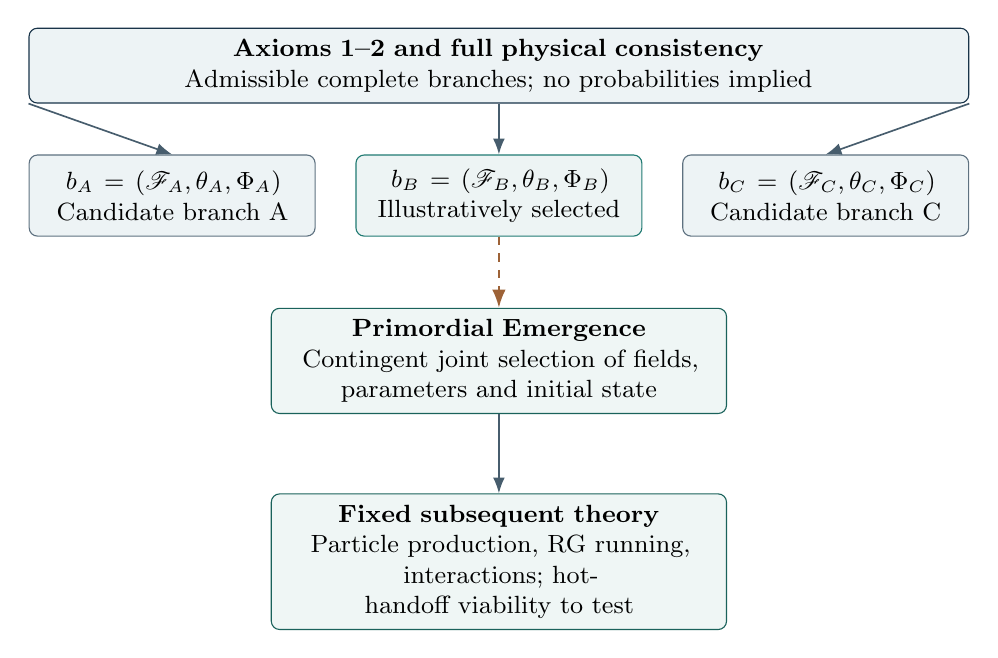
\begin{tikzpicture}[>=Latex,every node/.style={align=center,font=\small},
 pnode/.style={draw=deep!70,rounded corners=3pt,fill=paperblue,text width=3.35cm,minimum height=1.03cm,inner sep=4pt},
 gnode/.style={draw=seagreen!80!black,rounded corners=3pt,fill=seagreen!7,text width=5.5cm,minimum height=.95cm,inner sep=4pt},
 pathway/.style={->,semithick,draw=deep!80},
 chance/.style={->,thick,dashed,draw=caution}]
\node[draw=deep,rounded corners=3pt,fill=paperblue,text width=11.7cm,minimum height=.95cm] (set) at (0,0) {\textbf{Axioms 1--2 and full physical consistency}\\Admissible complete branches; no probabilities implied};
\node[pnode] (b1) at (-4.15,-1.65) {$b_A=(\mathscr F_A,\theta_A,\Phi_A)$\\Candidate branch A};
\node[pnode,draw=seagreen,fill=seagreen!8] (b2) at (0,-1.65) {$b_B=(\mathscr F_B,\theta_B,\Phi_B)$\\Illustratively selected};
\node[pnode] (b3) at (4.15,-1.65) {$b_C=(\mathscr F_C,\theta_C,\Phi_C)$\\Candidate branch C};
\draw[pathway] (set.south west) -- (b1.north);
\draw[pathway] (set.south) -- (b2.north);
\draw[pathway] (set.south east) -- (b3.north);
\node[gnode] (sel) at (0,-3.75) {\textbf{Primordial Emergence}\\Contingent joint selection of fields,\\parameters and initial state};
\draw[chance] (b2)-- (sel);
\node[gnode] (dyn) at (0,-6.3) {\textbf{Fixed subsequent theory}\\Particle production, RG running,\\interactions; hot-handoff viability to test};
\draw[pathway] (sel)--(dyn);
\end{tikzpicture}
\caption{\textbf{C002 logical branch diagram (not sampled data).} Different permissible configurations may carry different physically consistent field and parameter structures; selecting one is part of the founding contingent Primordial Emergence hypothesis. The arrows do \emph{not} represent measured probabilities, a derived transition amplitude, or proof that all three sample branches actually exist. Axioms 1--2 supply no prior physical clock.}\label{fig:c002branches}
\end{figure}

\subsection{What is fixed after the event, and what is not}
Once a complete post-emergence action $S_{\mathscr F_\star,\theta_\star}$ is fixed, it is the governing action for later particle production and composite formation. Neither ordinary interactions nor the appearance of new excitations cause a fresh stochastic draw of fundamental field species or independent Lagrangian parameters. This does \emph{not} mean particle populations are frozen, that a fundamental exotic field can never have existed, or that measured effective couplings are constant across renormalization scales. If the branch includes additional interacting exotic fields, it can produce their excitations; if an effective parameter depends on a dynamical modulus, a physical stabilization mechanism must still be checked (Section~\ref{sec:c001}).

The correct scientific claim is therefore \emph{joint contingent realization plus subsequent dynamical consistency}, not \emph{numerical prediction of all observed constants}. Dimensionless ratios are the important physical comparisons; arbitrary unit conventions do not become independently selectable observables. Different branches must each satisfy the relevant gauge, unitarity, stability, constraint and cosmological checks. The simultaneous all-Standard-Model-family emergence remains the founding hypothesis, not a constructed gauge-invariant state.

\subsection{The lean possibility goal and its remaining uncertainty}
A successful TUO existence result would show that $\mathscr B_{\rm hot}$ is nonempty through one physically connected origin-to-expanding-hot-state history, preferably a non-fine-tuned family. This does \emph{not} require a unique derivation of $\theta_\star$ or the exact observed cosmic energy. It also does not prove that a particular branch is ever actually realized, much less compute its probability. If TUO later asserts that successful emergence occurs with nonzero stochastic probability, it will need a measure or dynamical event model giving that claim physical content; the existence theorem alone is insufficient.

\begin{warningbox}
\textbf{C002 scientific status.} \emph{Clarified hypothesis:} Primordial Emergence contingently realizes one complete physically admissible field--constants--source sector, and later particle production obeys that selected theory. \emph{Exact mathematical point:} permissible branches do not determine their occurrence probabilities (Proposition~\ref{prop:c002measures}). \emph{Open physical obligations:} a realizable emergence state, source energy and initial expansion, an origin-to-hot-core evolution, and any asserted stochastic event law. This section adds \emph{no third axiom}, no pre-emergence clock, no empirical distribution of universes and no prediction of measured constants.
\end{warningbox}


\clearpage
\section{E008 --- A connected conditional Primordial Emergence-to-local-hot-state audit}\label{sec:e008}
\subsection{The simplification: E004 and E005 are alternative witnesses}
An important strategic error would be to assume the time-symmetric E004 Gaussian cloud must \emph{first} evolve into the E005 expanding-core configuration. Neither Axiom~1 nor Axiom~2 requires such a sequence: E003--E004 and E005 show \emph{different permissible post-emergence initial-data families}. Under TUO's C002 contingent-selection hypothesis, Primordial Emergence might select an E005-type initial geometry, matter population and field sector \emph{directly}. This selection itself remains an event premise; it is not deduced from a vanishing constraint, nor does this manoeuvre manufacture initial energy or expansion.

\begin{keybox}
\textbf{E008's positive result is conditional but genuinely connected.} Given an E005-compatible initially expanding central core populated by the E006 equal-and-opposite charged kinetic distributions, the \emph{same} gravitational/kinetic state has a continuous model evolution from initially photon-free charged matter to a radiation-rich FLRW core. E004 is not an intermediate stage. The founding event's occurrence, its unique microscopic Standard Model state, and the origin of nonzero $H_0$ are still assumed, not calculated.
\end{keybox}

\subsection{Conditional local bridge theorem}
On E005's spherical spatial slice, use the initial geometric and matter constraints
\begin{equation}
\gamma_{ij}=\psi^4\delta_{ij},\quad K_{ij}=-H(r)\gamma_{ij},\quad
\Delta\psi=-2\pi\widetilde\rho,\quad
\mathcal E=\frac{\widetilde\rho}{\psi^5}+\frac{3H^2}{8\pi},\quad
\mathcal J_r=\frac{H'}{4\pi}.
\end{equation}
These are \emph{exact} solutions of the Einstein initial constraints for E005's smooth shell data. Their central ball has $H_0>0$, positive energy, an isotropic massless distribution, and the same total $T^{\mu\nu}$ whether its energy is carried by the E006 oppositely charged initial particles or their reaction photons. Under the E006 stated reversible conservative kinetic closure, a single proper-time evolution obeys
\begin{equation}\label{eq:e008history}
\boxed{\frac{a(\tau)}{a_0}=\sqrt{1+2H_0\tau},\quad
\frac{\mathcal E(\tau)}{\mathcal E_0}=(1+2H_0\tau)^{-2},\quad
x(\tau)=\frac{1-e^{-4r(a/a_0-1)}}{3+e^{-4r(a/a_0-1)}}},\qquad r=\frac{\Gamma_0}{H_0}>0.
\end{equation}
Here $x(0)=0$, $\dot x>0$ for finite $\tau>0$, and $x\to 1/3$ in the declared classical massless Maxwell--Boltzmann model. Charge remains balanced and the \emph{total local stress tensor} is conserved; its proper radiation energy density redshifts as $a^{-4}$, so energy within a comoving region is \emph{not} constant. The conserved quantity for the idealized radiation evolution is $\mathcal E a^4$.

\textbf{Conditional proposition.} For an E005-compatible \emph{already populated, expanding} initial core with a positive E006 reaction rate and an appropriate regular mixed Einstein--reactive-matter development for a nonzero interval, there exists a continuous post-emergence trajectory with $H>0$, $\mathcal E>0$, $p=\mathcal E/3$ and increasing photon content. If the regular interval extends through the explicitly calculated model-conversion time, this state can reach any prescribed fraction $0<\eta<1$ of the model's chemical equilibrium. The E005 initial-data constraints hold on an open finite-dimensional parameter family, and the reaction rate is positive on an open range. This is a \emph{conditional weak local handoff}, not a global Einstein--Boltzmann theorem or an origin-from-empty-space theorem.

For $x=\eta/3$, direct algebra gives
\begin{equation}\label{eq:e008eta}
\boxed{\frac{\Delta a_\eta}{a_0}=
\frac{-\ln\!\left[(1-\eta)/(1+\eta/3)\right]}{4(\Gamma_0/H_0)},\qquad
\tau_\eta=\frac{(1+\Delta a_\eta/a_0)^2-1}{2H_0}.}
\end{equation}
The small positive $\Delta a_\eta/a_0$ must be retained numerically rather than subtracting floating-point values of $a/a_0$ extremely close to unity.

\subsection{A non-fitted 20-MeV quantitative consistency test}
Use E005's originally verified $(\mu,H_0L)=(0.5,0.01)$ and the E006 \emph{initial classical kinetic} temperature $k_BT_0=20$ MeV. The \emph{initial photon-free} Maxwell--Boltzmann pair distribution in the exact E006 closure has $\mathcal E_0=12(k_BT_0)^4/[\pi^2(\hbar c)^3]$, yielding $H_0\simeq158.86\,\mathrm{s}^{-1}$ from the initial Friedmann relation; $L\simeq18.871\,\mathrm{km}$ and central physical radius $R_0\simeq44.238\,\mathrm{km}$. This is a consistency scale of the \emph{specified toy state}; it is \emph{not} an exact equilibrated Standard Model bath. For example, at the same energy density the distinct $g_*=10.75$ full-equilibrium radiation formula would assign only $k_BT_{\rm equiv}\simeq15.31$ MeV.

The separately calculated physical Born-QED initial collision-rate estimate from E006 gives $\Gamma_0\simeq1.9532\times10^{18}\,\mathrm{s}^{-1}$ and $\Gamma_0/H_0\simeq1.2295\times10^{16}$. Equation~\eqref{eq:e008eta} gives $\tau_{99}\simeq6.26\times10^{-19}\,\mathrm s$ to reach 99\% of the \emph{model} photon-equilibrium content. E007's formal earliest shell-signal arrival is $\tau_{\rm sig}\simeq1.493\times10^{-4}\,\mathrm s$, so $\tau_{99}/\tau_{\rm sig}\simeq4.19\times10^{-15}$. Initial core proper energy is $1.47\times10^{45}$ J; its positive \emph{ADM} energy is about $1.14\times10^{48}$ J, reflecting the substantial explicitly prescribed shell. These values are not an inference that Primordial Emergence creates such energy, nor a retrospective fit to observed cosmic energy.

\begin{figure}[htbp]\centering\includegraphics[width=.92\linewidth]{E008_continuous_local_history.png}
\caption{E008 verified \emph{model} history. The chemical conversion within an already expanding, populated core is much faster than the formal earliest causal signal from the surrounding shell. The signal time does not guarantee global regularity or SM thermalization.}\label{fig:e008history}
\end{figure}
\begin{figure}[htbp]\centering\includegraphics[width=.88\linewidth]{E008_reaction_causal_margin.png}
\caption{The previously tested E006 physical Born-rate inputs at five classical pair kinetic temperatures yield a large ratio of the E005 formal shell-signal time to the \emph{model} chemical equilibration time. This is a kinetic plausibility screen, not a primordial event probability.}\label{fig:e008margin}
\end{figure}

\subsection{What the two axioms cannot establish, and what remains}
\textbf{Logical origin obstruction.} Axiom~1 supplies empty Euclidean $\R^3$ without a pre-existing time clock. Axiom~2 permits nontrivial field configurations satisfying typed zero-valued constraints. A model with no event/selection law and a model with an added contingent branch-realization prescription can satisfy these same axioms. Therefore \emph{they do not logically entail an actual emergence event}, its probability, the selected initial energy, or $H_0>0$. In particular the finite-dimensional openness of the E005 solution family does not supply a stochastic measure: a full-support branch-selection measure would be an \emph{additional physical assumption}, not a theorem of zero-residual admissibility. The founding Primordial Emergence hypothesis is deliberately not renamed Axiom~3.

\textbf{Microscopic and cosmological obstructions.} The all-Standard-Model-family simultaneous state has not been constructed as a gauge-physical microscopic quantum source; E006 does not solve exact quantum collision kinetics, coupled neutrino/photon transport, heavy species or the baryon asymmetry. A massless classical electron gas is not an exact finite-mass relativistic plasma. Although the formal E005 causal interval is large compared with its E006 reaction time, the core is only $H_0R_0/c\simeq0.02344$ Hubble radii wide. A persistent global hot-Big-Bang history and a rigorous duration for the coupled reactive gravitational shell evolution are not established. E008 thus connects \emph{conditional post-emergence stages}, but the full Primordial Emergence-to-conventional-hot-Big-Bang existence claim remains open.

\textbf{A no-shortcut check.} Consider an initially geodesic, twist-free normal congruence with $K_{ij}=0$, $\Lambda=0$ and $\varepsilon+3p>0$. Raychaudhuri's equation gives
\[
\dot\theta|_{\theta=0}=-\sigma_{ab}\sigma^{ab}-\frac{4\pi G}{c^2}(\varepsilon+3p)<0.
\]
Ordinary gravity therefore does not cause a momentarily stationary isotropic radiation configuration to immediately acquire \emph{positive normal-congruence} expansion. This is not a global no-go theorem for TUO, but it is another reason to avoid treating E004 as a mandatory dynamical predecessor of the E005 already expanding branch.

\begin{warningbox}
\textbf{E008 verdict.} A \emph{continuous effective-model history} from a selected, positive-energy, already expanding charged source to local hot FLRW radiation has been exhibited and independently checked. \emph{Not established}: spontaneous realization from the empty initial arena, microscopic all-Standard-Model gauge source, origin of $H_0$, exact QED/weak/QCD thermal history, baryogenesis and a persistent global cosmological handoff. The lean TUO possibility goal has a substantially clearer conditional witness, \emph{not} a completed physical origin theorem.
\end{warningbox}


\section{E009 --- Persistent cosmological handoff and the finite-origin boundary}\label{sec:e009}
\subsection{What a genuine global future theorem already proves}
A stronger endpoint than E005's small finite core is available in established general relativity, but its assumptions must not be silently transferred. For the \emph{spatially homogeneous, radiation-filled, noncompact} $\mathbb R^3$ Einstein--massless-Vlasov FLRW family, M.~Taylor proved that sufficiently small, compactly supported \emph{spherically symmetric perturbations of the FLRW background} have a future geodesically complete nonlinear development which remains appropriately close to FLRW~\cite{Taylor2024}. It follows that an \emph{open neighborhood of persistent expanding cosmological initial data} exists within those hypotheses. This is stronger than the E005 causally protected central interval. It does \textbf{not} prove a finite isolated Primordial Emergence forms the FLRW background: the background contains positive radiation density across all noncompact space, with infinite integrated proper matter energy, and the perturbations are \emph{of the background}, not localized matter replacing it.

\subsection{Finite-domain shielding and a geometric threshold}
For an exactly flat radiation-FLRW initial ball, define the dimensionless proper-radius parameter $u=H_0R_0/c$. As derived in E007, an inward light ray from the boundary formally reaches the center at
\[
\frac{a_{\rm sig}}{a_0}=1+u,\qquad H_0\tau_{\rm sig}=u+\frac{u^2}{2}.
\]
For approximately constant $g_{*s}$, cooling by a factor $q=T_0/T_*>1$ while remaining independent of the original shell requires $\boxed{u\ge q-1}$. This is a \emph{necessary condition only for pure causal shielding}, not a necessary condition for compatible coupled shell evolution or an early cosmological handoff. E005's representative $u=0.0234418$ implies an original-domain protected growth $a_{\rm sig}/a_0=1.0234418$. A twentyfold cooling protected solely by that mechanism would require $u\ge19$ and a much larger initial homogeneous region.

\begin{figure}[htbp]\centering\includegraphics[width=.82\linewidth]{E009_required_core_radius.png}
\caption{E009 exact causal-domain scale for two \emph{illustrative} thermal GR reference temperatures. No numerical observed-universe total-energy fit and no nonlinear TUO future simulation is involved.}\label{fig:e009radius}\end{figure}

The large domain has a rigorous geometric consequence. With future unit normal $n$, outward unit spatial normal $s$, $k_\pm=n\pm s$ and $c=1$, the FLRW areal-radius derivatives yield
\[
\boxed{\theta_\pm=\frac2R(HR\pm1)}.
\]
For $u>1$ both future expansions are positive: the sphere is \emph{anti-trapped} (past trapped). This is a cosmological feature, \emph{not} an isolated Schwarzschild black-hole diagnosis. The flat-FLRW Misner--Sharp ratio is $2GM_{\rm MS}/(c^2R)=u^2$; interpreting $u^2>1$ as proof of a black hole would be incorrect. Given a noncompact Cauchy slice, global hyperbolicity and null convergence, the time reverse of Penrose's singularity theorem implies that such a post-emergence spacetime cannot be \emph{past} null geodesically complete~\cite{PenroseReview}. This does \emph{not} imply future collapse; nor does it rule out TUO, whose Axiom~1 assumes no ordinary physical pre-emergence time. It prohibits a naive smooth, globally past-complete GR continuation from an already ordinary Minkowski arena. The classic Farhi--Guth obstacle concerns \emph{false-vacuum bubbles}, not a direct radiation-core no-go~\cite{FarhiGuth1987}.

\begin{figure}[htbp]\centering\includegraphics[width=.81\linewidth]{E009_null_expansions.png}
\caption{Exact flat-FLRW future radial null expansions against initial core radius in Hubble units. For $u>1$ the spheres are anti-trapped; $u=19$ marks the idealized twentyfold-cooling shielding threshold.}\label{fig:e009null}\end{figure}

\subsection{Why finite energy and everywhere-filled FLRW are different endpoints}
\textbf{Finite-propagation observation (conditional).} If the entire post-emergence matter distribution initially has compact support on a noncompact Cauchy slice, matter evolution is local and causal, and the post-emergence metric remains regular over a finite interval, then that source cannot populate \emph{every point} of noncompact $\mathbb R^3$ with nonzero homogeneous matter in finite regular time merely by local particle propagation. The causal image of the initial compact support cannot cover all of an unbounded slice in the stated setup. This does not exclude a \emph{finite} cosmological region, nonstandard global spacetime structure selected at emergence, or a separately justified global activation law. It does exclude treating E005's finite asymptotically flat matter distribution as already satisfying Taylor's \emph{everywhere FLRW background} hypotheses. The founding simultaneous appearance of all Standard Model fields and their antiparticles within a common initial volume remains different from global pre-population of the entire $\mathbb R^3$ background.

\begin{figure}[htbp]\centering\includegraphics[width=.81\linewidth]{E009_finite_support.png}
\caption{Schematic causal-support comparison (not a computed spacetime). Local finite-speed matter production from compact initial support is not automatically an everywhere-filled FLRW initial condition.}\label{fig:e009support}\end{figure}

\subsection{Non-fitted reference scales and the remaining dynamical task}
For ideal radiation $\varepsilon=(\pi^2/30)g_*(k_BT)^4/(\hbar c)^3$, flat Friedmann gives $H^2=8\pi G\varepsilon/(3c^2)$. E009's independently verified scales are:
\begin{center}\small\begin{tabular}{@{}lrr@{}}\toprule
Reference & $20$ MeV, $g_*=10.75$ & $10$ TeV, $g_*=106.75$\\\midrule
$H$ (s$^{-1}$) & $2.7094\times10^2$ & $2.1345\times10^{14}$\\
$c/H$ (m) & $1.1065\times10^6$ & $1.4045\times10^{-6}$\\
Radius $R_0$ for $u=19$ (m) & $2.1023\times10^7$ & $2.6686\times10^{-5}$\\\bottomrule\end{tabular}\end{center}
These are theoretical reference values for choosing a causal domain, not predictions of TUO's initial energy or size. The 10 TeV reference makes the full light Standard Model spectrum relativistic in the ideal-gas approximation, but neither the actual simultaneous gauge-physical quantum emergence state nor its coupled SM thermal kinetic evolution is constructed.

\begin{warningbox}
\textbf{E009 outcome: a real global endpoint theorem, but not a locality-to-globality bridge.} We now know that a globally radiation-filled FLRW massless-Vlasov branch has a rigorous open stable future under specified spherical perturbations, whereas E005/E008 give a finite already expanding core and short local conditional reaction history. Their starting data have different asymptotics. Pure causal shielding to large expansion factors demands large, anti-trapped initial FLRW regions, with consequent past-incompleteness conditions in ordinary GR. A genuinely \emph{localized} Primordial Emergence $\rightarrow$ a sustained adequate cosmological region remains open. The appropriate next work is a coupled finite core--shell Einstein--kinetic continuation theorem or simulation \emph{with physical post-emergence source data}, not importing a global background by assumption. Axiom~2 still does not enact a random event or derive initial $H_0>0$.
\end{warningbox}


\section{E010 --- Exact nonlinear shock-wave continuation of a finite hot core: scope and obstruction}\label{sec:e010}
\subsection{Why the E007 causal signal need not terminate radiation FLRW}
E007's finite-domain result $a_{\rm sig}/a_0=1+H_0R_0/c$ describes the interval during which the \emph{initial homogeneous core alone} guarantees uncontaminated expansion by domain of dependence. It is not a global breakdown time. An evolving exterior, if governed by physically consistent matching conditions, may allow an FLRW center to continue after its boundary becomes causally visible.

This possibility has a concrete external precedent. Smoller and Temple constructed exact, entropy-admissible \emph{Einstein--Euler} shock-wave cosmologies with an interior radiation-FLRW solution $p=\rho/3$, a moving nonvacuum shock interface and an exterior TOV-type region evolving inside a white-hole/black-hole spacetime~\cite{SmollerTemple2004,SmollerTemple2003}. This is a distinct initial-data class from E005's \emph{smooth} massless Einstein--Vlasov annulus. It is mathematically useful as an explicit full-spacetime continuation witness, not as a numerical evolution of the E005 shell or an origin mechanism derived by TUO.

\subsection{Physical interface and shock-matching equations}
A sharp, no-surface-layer timelike radiation-to-vacuum interface cannot obey normal stress conservation: a perfect fluid with $T^{\mu\nu}=(\rho+p)u^\mu u^\nu+pg^{\mu\nu}$ adjacent to vacuum requires $T^{\mu\nu}n_\nu=0$. For a spacelike interface normal $n$ and a timelike fluid velocity $u$, linear independence forces $u\cdot n=0$ and $p=0$, incompatible with $p=\rho/3>0$. The smooth E005 annulus and the nonvacuum Smoller--Temple shock resolve this interface issue in different ways.

In the radiation shock solution, use $G=c=1$, $\sigma=p/\rho=1/3$, $N=(H\bar r)^2$, and $u=\bar p/\rho$ with exterior pressure $\bar p$. Define $z=\ln N$. Equations (5.35)--(5.38) of Ref.~\cite{SmollerTemple2004} are
\begin{align}
\frac{du}{dz}&=-\frac{1+u}{2(1+3u)}\frac{(3u-1)(\sigma-u)N+6u(1+u)}{(\sigma-u)N+(1+u)},\\
\frac{d\ln\bar r}{dz}&=-\frac1{1+3u},\qquad
\frac{v_{\rm shock}}{c}=\sqrt{N}\frac{\sigma-u}{1+u}.
\end{align}
At the horizon-crossing interface, $N=1$, $u=0$. Set $\bar r_{\rm crit}=1$, $H_{\rm crit}=1$ and $t_{\rm crit}=1/2$. Then the radiation-FLRW time and enclosed Misner--Sharp mass obey
\begin{equation}\label{eq:e010mass}
\frac{t}{t_{\rm crit}}=\frac{\bar r}{\sqrt N},\qquad
\frac{M_{\rm shock}}{M_{\rm crit}}=\bar r N.
\end{equation}
The exterior is not an ordinary static star: its TOV radial coordinate is timelike inside the black-hole region. Interpreting $N>1$ as an isolated cosmological core having already collapsed would be a category error.

\begin{figure}[htbp]\centering\includegraphics[width=.82\linewidth]{E010_shock_hubble_radius.png}
\caption{E010's independent numerical reproduction of Smoller--Temple's exact fluid-shock matching equations. The shock remains outside the local Hubble radius until horizon crossing, while its influence becomes visible at the center earlier. This is \emph{not} an E005 Einstein--Vlasov evolution.}\label{fig:e010shock}\end{figure}

\subsection{What survives after the first boundary signal}
Normalize $a(t)=\sqrt{t/t_{\rm crit}}$ for radiation FLRW. From the limiting early comoving shock radius $r_* = \lim_{t\to0}\bar r(t)/a(t)$, the first ingoing signal reaches the center at $t_0$ satisfying $r_*=\int_0^{t_0}dt/a(t)=2\sqrt{t_0t_{\rm crit}}$. Therefore
\begin{equation}
\boxed{\frac{t_{\rm crit}}{t_0}=\left[\lim_{N\to\infty}(\bar r\sqrt N)\right]^{-1}\simeq3.6175,\quad
\frac{a(t_{\rm crit})}{a(t_0)}\simeq1.902.}
\end{equation}
This reproduces the radiation case of the rigorous $e^{\sqrt6/4}\le t_{\rm crit}/t_0\le e^{3/2}$ bounds of Theorem 9 in Ref.~\cite{SmollerTemple2004}. At central first visibility the shock is $1.5794$ Hubble radii away and has speed $0.4074c$; at horizon crossing its speed is $c/3$. Over the nonzero interval $t_0<t<t_{\rm crit}$, the exact matched spacetime \emph{still contains the expanding FLRW interior}, despite causal visibility of the boundary. With fixed relativistic degrees of freedom its equilibrium temperature proxy decreases by a factor $1.902$. No precise cosmological parameters are fitted.

\begin{figure}[htbp]\centering\includegraphics[width=.82\linewidth]{E010_post_signal_FLRW_growth.png}
\caption{The published exact matched model continues radiation FLRW after the boundary first becomes causally visible, unlike the claim that E007's first signal must terminate expansion. Thermal inverse-scale-factor behavior assumes an equilibrium equation of state.}\label{fig:e010continuation}\end{figure}

\subsection{The crucial incompatibility with TUO's finite origin}
Although the shock solution's enclosed mass is finite for every $t>0$, it diverges as $t\to0^+$; this follows from Eq.~\eqref{eq:e010mass} and is explicitly stated in Ref.~\cite[Section 8]{SmollerTemple2004}.
\begin{equation}
\boxed{M_{\rm shock}(t)<\infty\quad(t>0),\qquad
\lim_{t\to0^+}M_{\rm shock}(t)=\infty.}
\end{equation}
\begin{figure}[htbp]\centering\includegraphics[width=.82\linewidth]{E010_mass_backward_divergence.png}
\caption{Reconstructed backward divergence of the mass enclosed by the shock. This external exact cosmological model therefore does \emph{not} establish TUO's hypothesized finite-energy regular Primordial Emergence.}\label{fig:e010mass}\end{figure}
The Smoller--Temple solution contains a white-hole singularity; TUO does not assume an ordinary pre-emergence four-dimensional white-hole geometry. Neither the originally simultaneous full Standard Model quantum state nor E006's actual reactive collision distribution is derived by this perfect-fluid model. After $t_{\rm crit}$, the authors discuss a pressureless Oppenheimer--Snyder \emph{asymptotic approximation}; E010 does not assert an exact radiation fluid for all future time. It also does not imply that an E005 smooth shell would evolve into a Smoller--Temple shock.

\begin{keybox}
\textbf{E010 verdict.} The \emph{finite-boundary continuation objection is not universal}: an exact published nonlinear relativistic fluid solution keeps an expanding FLRW interior after the boundary becomes causally visible. E010 reproduces its radiation shock equations independently; the two mathematically equivalent ODE formulations agree to $1.7\times10^{-13}$ in $u$. \emph{But the tested shock model does not realize TUO's finite initial event: its backward mass diverges, it has a white-hole singularity, and it is not the E005--E006 kinetic system.} The strong Primordial Emergence-to-hot-Big-Bang theorem is still unproved.
\end{keybox}

\section{The current lean proof ledger and remaining bridge}\label{sec:ledger}
\begin{table}[htbp]\centering\footnotesize\renewcommand{\arraystretch}{0.91}
\begin{tabularx}{\linewidth}{@{}p{.21\linewidth}Yp{.23\linewidth}@{}}\toprule
\textbf{Link} & \textbf{Best supported result} & \textbf{Status}\\\midrule
Axioms 1--2 & Typed nontrivial zero-sum admissibility; theorems and physical analogues & Founding structure; interpretations verified\\
Primordial Emergence & Hypothesized simultaneous compact matter--antimatter--field configuration & Occurrence and microscopic state open\\
Localized positive energy & Gaussian free-wavepacket expectation $E\propto N/L$ & Conditional prepared-state benchmark\\
Exact sourced gravity & E003 Gaussian positive energy plus derived binding; $\mathcal H=\mathcal M=0$ & Exact classical initial data; $E_{\rm ADM}>0$\\
Open untrapped source family & E004 non-fitted region with selected conservative screens & Exact classical admissibility; no dynamic transition\\
Annihilation and production & Conserved reactions, conditional kinetic rates, unitary lattice volume effects & Standard channels + specified toy models; hot aftermath open\\
Reactive composition bridge & E006 reversible charged-to-photon kinetic closure inside E005; physical QED initial rates & Exact specified relaxation model; original event and geometry assumed\\
Expanding radiation core & E005 exact Einstein--Vlasov constraints and nonzero local FLRW development & Conditional post-emergence cosmology, prescribed radiation\\
Handoff causal audit & E007 exact protected-core scale limit $a_{\rm sig}/a_0=1+H_0R_0/c$ & Weak local entry only; extended hot cosmology open\\
One connected local branch & E008 shows E005--E006 share one conditional prepared charged-to-radiation history; $\tau_{99}\ll\tau_{\rm sig}$ & Verified in effective core model; origin and full SM handoff open\\
Persistent cosmological endpoint vs finite origin & E009: nonlinear future-stability theorem for global FLRW; causal/anti-trapped and finite-support limitations & Conditional global endpoint exists; local finite-origin bridge open\\
Exact radiation shock continuation & E010 reconstructs published Smoller--Temple Einstein--Euler dynamics with scale-factor growth $1.902$ after first boundary signal & Boundary continuation exists in a different exact model; white-hole singularity and divergent backward mass exclude finite regular TUO origin\\
Quantum-correlated admissibility & N001 exact singlet, color-singlet analogy and constrained relational-clock toy & Checked quantum examples; no primordial gauge-gravity state or new origin law\\
Gauge-physical correlated quantum seed & N002 finite $U(1)$ lattice physical state, positive excitation energy, exact short-time multi-pair amplitude and stationary-vacuum control & Exact regulated toy $1+1$D quantum result; not the complete Standard Model origin\\
Two-sided 3D hot-plasma overlap & N004 open local interaction/compactness window, reduced reaction ODE, 1-TeV backward comoving mismatch & Necessary-condition overlap; full common forward/backward history still open\\
3D energy-moment and one-source intersection & N005 exact massless virial theorem, finite positive Einstein initial data, positive open reduced energy/composition screen & Rigorous stress and initial constraints; approximate post-slice dynamics; hot FLRW handoff open\\
Reversible collision and fluid consistency & N006 uses same finite source in conservative 3D relativistic radiation fluid; reversible weak $T^9$ thermal-bath moment closure with inverse-reaction control & Numerical continuum-fluid comparison and assumed bath closure; not full SM Boltzmann or Einstein evolution\\
Spectrum selection/closure & S001 fixed-field interpretation, conditional invariant-subspace criterion and exotic-mixing test & Post-emergence QFT principle; primordial selection \emph{not derived}\\
Constants and contingent selection & C001 coupling nonuniqueness; C002 joint branch premise and exact probability-underdetermination result & Contingent selection postulated; no event law, measure or numerical prediction\\
\textbf{Complete Primordial Emergence-to-hot-Big-Bang history} & No event/transition law or globally extensive SM radiation evolution & \textbf{NOT established}\\\bottomrule
\end{tabularx}
\caption{Evidence ledger for the lean possibility programme. ``Exact'' always means exact within the stated post-emergence equations and assigned matter content.}\label{tab:officialledger}
\end{table}

The explicit three-gate roadmap is given in Section~\ref{sec:m001}. N002 now supplies an additional exact, small gauge-physical quantum witness for M1 (Section~\ref{sec:n002}), but a single complete $3+1$-dimensional Standard-Model-compatible initial state and its event law remain open. Quantum-correlated states sharpen the initial-state question (Section~\ref{sec:n001-axiom2}) without supplying a spontaneous-emergence mechanism. The shortest remaining scientific programme is \textbf{not} the derivation of every Standard Model scattering process or a forced E004-to-E005 transition. It is (i) a physically justified, gauge/quantum-consistent \emph{realization} of a complete Primordial Emergence branch that contains the necessary positive energy and nonzero expansion, rather than simply assigning that branch a nonzero chance, and (ii) a valid interacting continuation broad enough to serve as a conventional hot-Big-Bang handoff. E008 already connects a chosen E005-compatible populated charged state to a locally radiation-rich FLRW state within a specified reactive kinetic model. This connected witness does not generate its own initial population, $H_0$, or the event law; nor does it establish a global Einstein--Boltzmann development. E009 supplies a rigorous \emph{global} future-stability endpoint for a different initial-data class. E010 separately shows published \emph{exact shock continuation} of an expanding finite FLRW core beyond first causal visibility, but its white-hole origin and divergent backward mass exclude it as an E005 or finite Primordial Emergence history. Any completed construction must preserve the selected S001 field-sector dynamics and exact gauge/gravitational constraints. A pre-baryogenesis handoff may legitimately defer baryon-asymmetry physics to the subsequent theory, but it must explicitly specify the required later mechanism.

\begin{keybox}
\textbf{Current defensible conclusion (10 November 2026).} \emph{Nontrivial-zero constrained positive-energy sources exist in specified classical theories. A finite expanding radiation core is admissible and follows radiation-FLRW locally, while a specified conservative reversible kinetic model converts balanced charged matter into photons within that core. E008 demonstrates that these pieces describe one connected \emph{conditional post-emergence local history}, not two unrelated constructed stages.} This is not proof that Primordial Emergence generates or realizes the populated expanding core, nor that the core forms a full hot-Big-Bang history. E009 establishes a distinct global stable radiation-FLRW endpoint; E010 reproduces an exact finite shock-wave continuation beyond the first central boundary signal, but its singular origin and divergent backward mass do not realize Primordial Emergence. No observed total energy was fitted. That boundary is the principal remaining test of TUO.
\end{keybox}

\section{M001 --- Only three essential milestones remain}\label{sec:m001}
The intended TUO result is a \emph{lean conditional existence proof}, not unique prediction of the observed cosmic energy, constants, or the full thermal history. With quantum gravity left open, the minimal decisive programme is a \emph{single compatible chain} through these three milestones:
\begin{table}[htbp]\centering\small
\begin{tabularx}{\linewidth}{@{}p{.21\linewidth}Yp{.26\linewidth}@{}}\toprule
\textbf{Milestone} & \textbf{Necessary pass condition} & \textbf{Current gap}\\\midrule
\textbf{M1. Complete Primordial Emergence state} & Exhibit one normalizable, finite, nontrivial correlated post-emergence quantum state with a complete Standard-Model-compatible field sector, exact local gauge constraints and designated neutral charges, and positive energy. The simultaneous localized emergence itself remains a clearly stated founding hypothesis. & N001 and N002 now show exact small quantum witnesses; the complete $3+1$D Standard-Model gauge-dressed quantum state and event law are not built.\\
\textbf{M2. Consistent initial expansion} & Map the \emph{same} matter--field quantum state to a physically justified stress tensor and complete gravitational initial data with $H>0$ and controlled classical/semiclassical applicability, rather than assigning an unrelated E005 core. & E003--E005 give solutions for prescribed sources, not for M1's source. The emergence of geometry itself is not derived.\\
\textbf{M3. Sustained hot-Big-Bang handoff} & Show one compatible family follows causal energy--momentum conserving evolution to an adequately extensive hot, radiation-rich, near-equilibrium state with relevant particle content and a defensible continuation into conventional cosmology. & E006--E008 give a local conditional bridge; E009--E010 show possible endpoints or interfaces in different models, not the full common history.\\\bottomrule
\end{tabularx}
\caption{TUO's shortest remaining non-fitted existence roadmap. Milestones must hold for one compatible physical family rather than for unrelated examples.}\label{tab:m001}
\end{table}

\begin{warningbox}
\textbf{The quantum-gravity boundary.} A full microscopic derivation of spacetime is \emph{not} stipulated as a prerequisite for this conditional result: it may be enough to show an explicit quantum source whose expectation stress and matter correlations admit controlled classical Einstein initial data and a valid evolution. This does \emph{not} explain why spacetime exists. If the only bridge is to \emph{postulate} the geometry and its expansion independently, M2 has not been closed. Nor can Axioms 1--2 alone turn admissibility into a proof that the contingent event actually happens or carries a specified probability.
\end{warningbox}

The earlier Q001/E004 and E005 initial-data families need not be forced into a historical sequence. An admissible Primordial Emergence branch may begin directly with a justified expanding state; what cannot be omitted is the link between that \emph{same complete matter source}, its geometry and its subsequent hot evolution. The handoff may occur before conventional baryogenesis if the required later baryon history is specified as part of the subsequent physical theory. No quantum-gravity prediction, exact relic abundances or observed-total-energy fit is claimed by this limited objective.


\section{N002 --- Exact Gauss-physical correlated seed and controlled pair dynamics}\label{sec:n002}
\subsection{Why a new calculation was necessary}
TUO's contingent-branch hypothesis does not uniquely determine couplings, initial energy or the initial quantum state. Nor is it enough to treat a list of particles as if gauge links and Gauss constraints were independent afterthoughts. N002 therefore tests the nontrivial \emph{post-emergence} step in a conventional interacting lattice gauge theory: can a neutral, normalized, physically constrained, correlated matter--field initial state carry positive excitation energy and dynamically populate additional particle--antiparticle sectors? It does \emph{not} test spontaneous formation from Axiom~1's empty, clock-free spatial arena. Its $1+1$-dimensional $U(1)$ gauge field has no independent propagating transverse photons and is not a complete Standard Model substitute. The construction uses the standard staggered Schwinger-model Hamiltonian and open-boundary Gauss law \cite{N002SchwingerPTEP,N002SchwingerPRD}.

\subsection{Constraint-physical Hilbert space and an exact seed}
For eight staggered sites, $n_j=\chi_j^\dagger\chi_j$, and $b_j=[1-(-1)^j]/2$ the odd-site filled staggered reference, impose zero exterior link flux and the operator Gauss laws
\begin{equation}
\widehat G_j=L_j-L_{j-1}-(n_j-b_j),\quad
\widehat G_j|\Psi_{\rm phys}\rangle=0,\quad
L_j=\sum_{k\le j}(n_k-b_k).
\label{eq:n002gauss}
\end{equation}
With total charge zero and half filling, the physical basis has $\binom84=70$ states; each fermionic occupation configuration fixes \emph{every} internal electric-flux string. Consider the interacting Hamiltonian
\begin{equation}
\begin{aligned}
H={}&-w\sum_{j=0}^{6}(\chi_j^\dagger U_j\chi_{j+1}+\chi_{j+1}^\dagger U_j^\dagger\chi_j)\\
&+m\sum_{j=0}^{7}(-1)^j(n_j-b_j)+J\sum_{j=0}^{6}L_j^2,
\end{aligned}\label{eq:n002ham}
\end{equation}
where $J=g^2a/2>0$, $[L_j,U_k]=\delta_{jk}U_k$, and $w,m>0$. The gauge link moves with each nearest-neighbor charge transfer, so $[G_j,H]=0$. Set $|s_A\rangle$ by moving the occupied odd reference site $3\to4$, and $|s_B\rangle$ by moving $5\to2$, with the \emph{distinct} electric strings determined by Eq.~\eqref{eq:n002gauss}. The normalized correlated seed
\begin{equation}
|\Psi_0\rangle=\frac{|s_A\rangle_{\rm phys}+|s_B\rangle_{\rm phys}}{\sqrt2}
\label{eq:n002seed}
\end{equation}
is sharply net-neutral and annihilated by \emph{each local Gauss generator}, not merely its expectation. It has one staggered particle--antiparticle pair and $\langle H\rangle_0=2m+2J$. Since $w>0$ connects it to other pair sectors, it is not the interacting ground state: $\langle H\rangle_0-E_{\rm min}>0$ for this finite theory. The flux-string correlations are exact in the extended matter--link kinematic representation, but entanglement entropy in a constrained gauge system depends on the chosen factorization.

\subsection{A positive multi-pair probability without extra energy}
Let $P_{\ge2}$ project onto the two-or-more-pair configurations. A direct, exact short-time expansion gives
\begin{equation}
\boxed{\mathbb P_{\ge2}(t)=\|P_{\ge2}e^{-iHt/\hbar}|\Psi_0\rangle\|^2
=\frac72\left(\frac{wt}{\hbar}\right)^2+O(t^4).}
\label{eq:n002pair}
\end{equation}
The coefficient follows from $\|P_{\ge2}H|\Psi_0\rangle\|^2=7w^2/2$, with vanishing odd powers for this real-representable Hamiltonian, state and projector. The leading term is independent of $m,J$: for every fixed finite $m,J$ and $w>0$ this specific quantum model has an interval $t>0$ with nonzero probability for additional pairs. The fact \emph{does not} imply a physical probability for primordial occurrence. Unitary evolution preserves the full energy and produces additional particles only by redistributing the initial quantum energy.

\begin{figure}[htbp]\centering\includegraphics[width=.86\linewidth]{N002_pair_creation.png}
\caption{N002 exact 70-dimensional quantum evolution for three independently selected $J/w$ ratios at $m/w=0.65$. The expected pair number can rise beyond the initial value of one, without changing total energy or violating local Gauss laws. These are illustrative toy parameters, not a fit to our universe or a measure of chance selection.}\label{fig:n002pair}
\end{figure}
\begin{figure}[htbp]\centering\includegraphics[width=.94\linewidth]{N002_spread_correlations.png}
\caption{The model's excitations can spread spatially, and matter--link correlations evolve. These are \emph{lattice} observables; they do not yield a cosmological Hubble parameter or FLRW expansion. The gauge-link entropy uses an extended-Hilbert-space split.}\label{fig:n002spread}
\end{figure}
For $J/w=(0.18,0.55,1.25)$ and fixed $m/w=0.65$, the maximum expected pair numbers on $0\le tw/\hbar\le9$ are $(2.108,2.038,1.941)$; norm and energy violations are at numerical roundoff. Independent sparse evolution for $N=(8,10,12)$ and dimensions $(70,252,924)$ reproduces gauge-physical pair dynamics. The leading pair-sector coefficient grows with size because the entire bare reference state is dynamical, so it must \emph{not} be interpreted as a long-range cascade initiated by one local pair.

\subsection{The necessary failure control and the better meson candidate}
The staggered reference $|b\rangle$ is \emph{not} the true interacting ground state when $w\ne0$. It also evolves into multi-pair configurations: at $J/w=0.55$ and $tw/\hbar=1$, $\langle N_{\rm pair}\rangle_{|b\rangle}\simeq1.924$, compared to $\simeq2.032$ for the prepared correlated one-pair seed. Thus one \emph{cannot} claim the extra pairs were wholly caused by a new seed-triggered chain reaction. The exact interacting ground state remains stationary, as it must.
\begin{figure}[htbp]\centering\includegraphics[width=.90\linewidth]{N002_vacuum_control.png}
\caption{N002 negative control: the nonstationary bare staggered reference itself generates pair configurations, while the actual interacting ground is stationary. This rules out attributing all pair production to the originally prepared pair.}\label{fig:n002control}
\end{figure}
A cleaner physical source benchmark is the \emph{gauge-invariant} adjacent meson insertion $\mathcal O=\chi_4^\dagger U_4\chi_5$ on the exact interacting ground $|\Omega\rangle$, followed by normalization: $|\Psi_M\rangle=\mathcal O|\Omega\rangle/\|\mathcal O|\Omega\rangle\|$. It has $E_M=\langle\Psi_M|H|\Psi_M\rangle-E_{\rm min}=2.827499w>0$ at the representative parameters. Its local excitation profile evolves while $|\Omega\rangle$ does not, giving a physical local-response witness distinct from a background quench.
\begin{figure}[htbp]\centering\includegraphics[width=.90\linewidth]{N002_mesonic_spread_control.png}
\caption{Exact response of the normalized gauge-dressed meson excitation \emph{relative to the stationary interacting ground}. Signed local excitation-density differences propagate in a finite chain; they do not establish a sustained cosmic thermal plasma.}\label{fig:n002meson}
\end{figure}

\begin{warningbox}
\textbf{N002 result and limits.} This partially advances M1: an explicit \emph{small} normalizable physical quantum state, genuine local Gauss constraints, nontrivial matter--gauge correlation, positive excitation energy, and exact interacting evolution have been constructed with reproducible controls. However the model is $1+1$-dimensional $U(1)$, uses a pre-existing Hamiltonian and time, and has neither complete Standard Model fields, a spontaneous creation law, propagating physical photons, global thermodynamics, nor gravity. The ground-state control \emph{refutes} interpreting all its pair multiplication as a seed-caused self-sustaining cascade. Different $J/w$ ratios are specified branches, not a derived chance distribution. \emph{M1 is not complete; M2 and M3 remain open.}
\end{warningbox}


\section{N004 --- Two-sided three-dimensional hot-handoff screen}\label{sec:n004}
The suggested research strategy is to \emph{meet in the middle}: propagate the known hot-Big-Bang plasma requirements \emph{backward} and a localized quantum matter--antimatter system \emph{forward}, demanding an actual overlap of physical conditions. This section records N004 as a reproducible \emph{necessary-condition screen}, not an exact $3+1$D Standard Model quantum collision simulation. The earlier N003 external-pulse calculation shows controllable energy redistribution into additional gauge-physical pair sectors in the finite N002 theory, but its parameter $w$ is not calibrated to the extreme Planck-localized Q001 energy. We continue to treat field species, dimensionless constants and initial energy as TUO-contingent branch choices, not inevitable observed numbers.

\subsection{Local open thermalization window at 20 MeV}
For a chosen Standard Model-compatible reference radiation plasma, take $g_*=10.75$ at equilibrium-equivalent $T=20\,\mathrm{MeV}$ \cite{N004Hot,N004Nu}. The radiation density and GR reference expansion rate obey
\begin{equation}\label{eq:n004back}
\epsilon=\frac{\pi^2g_* T^4}{30\hbar^3c^3},\qquad
H^2=\frac{8\pi G\epsilon}{3c^2},\qquad H_{20}=270.94\,\mathrm{s}^{-1}.
\end{equation}
Here $T$ represents thermal energy (not kelvin). Define $u=HR/c$, an interaction depth $\mathcal N_\nu=\Gamma_\nu R/c$, and the order-of-magnitude weak interaction estimate $\Gamma_\nu=C_\nu G_F^2T^5/\hbar$ in natural energy units. $C_\nu=0.1$ is a deliberately conservative illustrative choice, \emph{not} an exact full weak collision integral. Requiring ten interaction times before a light-crossing and imposing the selected mild-compactness screen $u<0.1$ yields the analytically \emph{open} interval
\begin{equation}\label{eq:n004window}
\boxed{\frac{10c}{\Gamma_\nu}<R<0.1\frac{c}{H},\qquad
\text{possible iff}\quad\Gamma_\nu/H>100.}
\end{equation}
With $M_{\rm Pl}$ the unreduced Planck mass, $\Gamma_\nu/H\sim C_\nu G_F(\boldsymbol\theta)^2M_{\rm Pl}(\boldsymbol\theta)T^3/[1.66\sqrt{g_*(\boldsymbol\theta,T)}]$ makes the dependence on contingently selected constants explicit. At 20 MeV, $\Gamma_\nu/H=244.1$ for $C_\nu=0.1$. Hence $45.3\,\mathrm{km}<R<110.6\,\mathrm{km}$ passes these local necessary screens. $R=60\,$km has $u=0.0542$, $\mathcal N_\nu=13.24$, and homogeneous radiation energy $E_{\rm core}=1.068\times10^{46}\,\mathrm{J}$. Its uniform-density mass-equivalent compactness $2GE_{\rm core}/(c^4R)=u^2=0.00294$ is modest. It is \emph{not} a computed ADM mass or proof of stable asymptotically flat fluid evolution. Such an energy is not supplied by Q001's $1.405\times10^{11}$-J free-wavepacket benchmark; the two energy budgets are explicitly distinct.
\begin{figure}[htbp]\centering\includegraphics[width=.87\linewidth]{N004_thermal_window.png}
\caption{N004 two-sided feasibility screen at 20 MeV. A nonempty size window admits many characteristic weak interactions with moderate $HR/c$. The reference input couplings are one possible TUO branch, and $u<0.1$ is a selected diagnostic rather than an objective law.}\label{fig:n004window}\end{figure}

\subsection{One local forward kinetic history, with precise limits}
As an intentionally reduced energy-conserving \emph{composition} closure, assume a rapid electromagnetic partition between $e^\pm$ and photons followed by weak exchange with the neutrino sector. Let $f_e+f_\gamma+f_\nu=1$, $f_e=\eta(1-f_\nu)$, $\eta=3.5/5.5$, $f_\nu(0)=0$, and $f_{\nu,\rm eq}=5.25/10.75$. Within a \emph{prescribed} radiation-FLRW central domain with $a/a_0=(1+2H_0\tau)^{1/2}$, the simplified weak rate $\Gamma_\nu(\tau)=\Gamma_{\nu0}(a/a_0)^{-5}$ gives
\begin{equation}\label{eq:n004forward}
\boxed{ f_\nu(\tau)=f_{\nu,\rm eq}\!\left[1-\exp\left(-\eta\frac{\Gamma_{\nu0}}{3H_0}\big[1-(1+2H_0\tau)^{-3/2}\big]\right)\right].}
\end{equation}
At $R=60\,$km, N004 finds $\tau_{99}=118.22\,\mu\mathrm{s}$ for the neutrino \emph{energy fraction} in this closure, while the first formal boundary signal is $\tau_{\rm sig}=205.56\,\mu\mathrm{s}$ using E007's central null-cone formula. At that boundary signal the equilibrium-fraction completion is about 99.95\%, and the central scale ratio is only $a_{\rm sig}/a_0=1.05423$. Equation~\eqref{eq:n004forward} agrees with a high-precision numerical ODE solver to $2.9\times10^{-13}$ in fractional energy. The electromagnetic fast stage, weak relaxation kernel, initial stress density and geometry are \emph{assigned}; this is not the full SM collision operator or an evolution of N002/N003's quantum state. It does not certify persistence beyond the boundary.
\begin{figure}[htbp]\centering\includegraphics[width=.87\linewidth]{N004_forward_energy_exchange.png}
\caption{Analytical and numerical solution of a specified reduced forward energy-sharing model, not a full gauge quantum-field or Einstein--Boltzmann calculation. A rapidly equilibrated electromagnetic sector and a fixed expanding central background are assumed.}\label{fig:n004forward}\end{figure}

\subsection{Backward high-temperature check exposes a separate domain problem}
A full Standard Model-compatible high-energy branch should also confront the electroweak era, with the measured Standard Model crossover near 159.5 GeV \cite{N004EW}. A conventional comparison at 1 TeV ($g_*=g_{*s}=106.75$) gives adiabatic entropy-domain scaling
\begin{equation}\label{eq:n004rewind}
\frac{a_{20}}{a_{1\rm TeV}}=\frac{1\,\mathrm{TeV}}{20\,\mathrm{MeV}}\left(\frac{106.75}{10.75}\right)^{1/3}=1.0747\times10^5,
\qquad \frac{u_{1\rm TeV}}{u_{20}}=7.3304\times10^4.
\end{equation}
The 60-km 20-MeV region maps backward to $R_{1\rm TeV}=0.558\,$m and $u_{1\rm TeV}\simeq3975$. In contrast, an initially \emph{sub-Hubble} 1-TeV region maps to at most $R_{20}=15.1\,$m and $0.00333$ characteristic weak interaction times per crossing for $C_\nu=0.1$: far below the chosen late ten-interaction condition. \emph{This is a conditional negative test of unassisted single-comoving-domain scaling, not a theorem against a compatible nonlinear evolving exterior, domain growth or differently selected couplings.} Large expanding super-Hubble spheres may be anti-trapped; they are not automatically black holes, but their early gravitational structure requires a separate origin account.
\begin{figure}[htbp]\centering\includegraphics[width=.86\linewidth]{N004_backward_mismatch.png}
\caption{Backward comoving-FLRW domain audit from 20 MeV to 1 TeV: a late local reaction-feasible region is highly super-Hubble at 1 TeV under simple adiabatic support evolution. This comparison cannot be reinterpreted as a directly simulated localized emergence.}\label{fig:n004rewind}\end{figure}

\subsection{Why a fixed arena still needs a radiation pressure-work ledger}
On a fixed background, purely free-spreading packets of conserved total energy have $\epsilon\propto R^{-3}$ for an expanding effective volume. Radiation-FLRW obeys $\epsilon\propto a^{-4}$. A physical finite core can reproduce the same \emph{interior} $R^{-4}$ scaling in principle only if it exchanges work/energy with its exterior:
\begin{equation}\label{eq:n004work}
\mathrm d E_{\rm core}=-p\,\mathrm d V=-\frac{E_{\rm core}}{3V}\mathrm dV
\quad\Longrightarrow\quad E_{\rm core}\propto R^{-1},\quad \epsilon_{\rm core}\propto R^{-4}.
\end{equation}
This is a conservation identity contingent on the adiabatic radiation-fluid assumptions, \emph{not} a derived effective GR metric or a demonstration that particle spreading is observed FLRW expansion. It states the energy-transfer condition a QGD-like fixed-background interpretation would have to meet.

\begin{warningbox}
\textbf{N004 conclusion.} We have established an \emph{open local finite-size interaction/compactness window} and an exact solution of a chosen reduced forward composition model, while identifying a stringent \emph{backward comoving-domain mismatch}. These are genuine, reproducible necessary-condition results. They do \emph{not} prove that one complete gauge-physical $3+1$D state supplies the displayed radiation energy, that a Primordial Emergence event occurs, or that the core+shell system persists to standard cosmology. M1--M3 remain incomplete; the next calculation must evolve the same selected quantum source, its collision stress and an actual finite boundary/exterior.
\end{warningbox}



\clearpage
\section{N005 --- A three-dimensional forward--backward possibility intersection}\label{sec:n005}
This section respects TUO's \emph{possibility} rather than unique-number-fitting target. The backward calculation fixes a minimal, well-understood hot radiation \emph{checkpoint}; the forward calculation asks whether a single finite positive-energy state can meet an open subset of these requirements. We do not require an initially thermal $1\,$TeV bulk merely because an initial state may excite all Standard Model field species: a heavy species can be present as a rare \emph{nonthermal} excitation. Constructing a full physical all-species gauge state, and the observed baryon history, remain separate tasks.

\subsection{Exact fixed-space dynamical spreading, without imposing an initial Hubble parameter}
For symmetric $T^{\mu\nu}$ of a massless post-emergence kinetic system with finite total energy $E=\int T^{00}d^3x>0$, assume $\partial_\mu T^{\mu\nu}=0$, $T^\mu{}_{\mu}=0$ and sufficiently rapid decay. Set $I(t)=\int r^2 T^{00}(t,\bm x)d^3x$. Twice integrating by parts yields the exact identity
\begin{equation}\label{eq:n005virial}
\boxed{\quad I''(t)=2c^2\!\int\! T^{ii}(t,\bm x)d^3x=2c^2E,\qquad R_E^2(t)=\frac{I(t)}{E}.\quad}
\end{equation}
For zero initial integrated radial energy flux, $I'(0)=0$, therefore
\begin{equation}\label{eq:n005spread}
\boxed{R_E(t)=\sqrt{R_E^2(0)+c^2t^2},\qquad H_E(t)\equiv \frac{\dot R_E}{R_E}=\frac{c^2t}{R_E^2(0)+c^2t^2}.}
\end{equation}
This is a \emph{spatial energy-moment expansion}, not FLRW $H$ or cosmological redshift. It does not create energy. It remains valid in a relativistic collision model conserving total stress--energy and tracelessness, but mass/trace anomalies change the exact coefficient. For an initially radial, isotropic, massless kinetic source $\epsilon_0(r)$, its \emph{collisionless} continuation is exactly
\begin{equation}\label{eq:n005radial}
\epsilon(r,t)=\frac12\int_{-1}^1\epsilon_0\big(\sqrt{r^2+c^2t^2-2rct\mu}\big)d\mu,\qquad\epsilon(0,t)=\epsilon_0(ct).
\end{equation}
\begin{figure}[htbp]\centering\includegraphics[width=.88\linewidth]{N005_forward_exact_3D.png}
\caption{N005 exact massless-energy spreading with no inserted initial positive Hubble flow (left), and central \emph{equilibrium-equivalent} energy-density temperature for the same freely propagated source (right). Not a thermal distribution or FLRW metric.}\label{fig:n005forward}\end{figure}

\subsection{Same positive source and the exact classical gravitational initial constraints}
The source admits a \emph{time-symmetric} regular classical initial-data realization: choose $K_{ij}=0$, $j_i=0$, $\gamma_{ij}=\psi^4\delta_{ij}$, and $\rho_N=(2\pi L^2)^{-3/2}e^{-r^2/(2L^2)}$ with
\begin{equation}\label{eq:n005GR}
\boxed{\psi(r)=1+\frac{GM}{2c^2r}\operatorname{erf}\!\left(\frac{r}{\sqrt2L}\right),\quad
\epsilon_{\rm GR}(r)=\frac{Mc^2\rho_N(r)}{\psi(r)^5}>0,\quad
E_{\rm ADM}=Mc^2>0.}
\end{equation}
Then $\Delta\psi=-2\pi GM\rho_N/c^2$, ${}^{(3)}R=16\pi G\epsilon_{\rm GR}/c^4$, and the momentum constraint holds identically. A positive isotropic massless kinetic distribution realizes the initial $\epsilon$, $j_i=0$, $p=\epsilon/3$; $E_{\rm proper}=Mc^2+GM^2/(2\sqrt\pi L)$. The Gaussian has finite energy but noncompact support. Multiplying $\rho_N$ by a smooth cutoff equal to $1$ for $r\le6L$ and $0$ for $r\ge7L$ gives a \emph{strictly compact matter source}; resolve the same Poisson equation for $\psi$ to preserve the exact constraints. The discarded normalized Gaussian mass beyond $6L$ is $7.49\times10^{-8}$, and the central forward history through the chosen $t_*$ samples only $r\le ct_*<L$; hence its strict inequalities survive the cutoff by continuity. The exterior gravitational field need not have compact support. \emph{The constrained GR initial slice is exact; its subsequent full Einstein--Vlasov evolution has not been identified with the separate flat free-streaming calculation.}
\begin{figure}[htbp]\centering\includegraphics[width=.88\linewidth]{N005_initial_Einstein_constraint.png}
\caption{The same initial positive radial energy density has a regular exact Einstein constraint realization with positive ADM energy and no initial expansion assigned ($K_{ij}=0$). This is not an evolved quantum-gravity theory.}\label{fig:n005GR}\end{figure}

\subsection{Backward energy-density target and forward reduced species-transfer screen}
The backward reference is an \emph{equilibrium-equivalent} $20\,$MeV radiation density with $g_*=10.75$. Choose a central ray reaching the origin at $t_*$ and propagate the \emph{same} initial $\epsilon_{\rm GR}(r)$ in Eq.~\eqref{eq:n005radial} as a weak-gravity kinetic comparator. For a positive energy-label relaxation closure, with a fast electromagnetic partition \emph{assumed}, put $f_{\nu,\rm eq}=5.25/10.75$, $\eta=3.5/5.5$ and
\begin{equation}\label{eq:n005rate}
\frac{df_\nu}{dt}=\eta\Gamma_\nu(\epsilon)\big(f_{\nu,\rm eq}-f_\nu\big),\quad
\Gamma_\nu=C_\nu\frac{G_F^2}{\hbar}T_{\rm eq}(\epsilon)^5,\quad C_\nu=0.1,\quad
T_{\rm eq}(\epsilon)=20\,\mathrm{MeV}\left(\frac{\epsilon}{\epsilon_{20}}\right)^{1/4}.
\end{equation}
As the ray has $r(t)=c(t_*-t)$, $f_\nu(t_*,0)/f_{\nu,\rm eq}=1-\exp[-\eta\int_0^{t_*}\Gamma_\nu(t,c(t_*-t))dt]$. This is the \emph{exact solution of that specific reduced relaxation model} on the exact collisionless energy profile, \emph{not} a complete Standard Model scattering or QED/weak Boltzmann calculation. The transfer mechanism conserves modeled energy--momentum by relabeling energy streams, but actual $e^+e^-\leftrightarrow\nu\bar\nu$ processes involve two-body kinematics, angular integrals, blocking and inverse reactions. It does not establish a thermal particle spectrum.

For the checked representative, choose $R_E(0)\simeq90\,$km ($L=90/\sqrt3\,$km), $t_*=0.150\,$ms and select $M$ to enforce the backward equality $\epsilon_{\rm GR}(ct_*)=\epsilon_{20}$. This determines a positive source; it does not fit TUO's selected constants or infer an emergence probability. Results:
\begin{equation}\label{eq:n005numbers}
\boxed{\begin{gathered}
E_{\rm proper}=3.8392\times10^{46}\,\mathrm{J},\qquad
E_{\rm ADM}=3.8326\times10^{46}\,\mathrm{J},\\
\frac{2GM}{c^2(90\,\mathrm{km})}=0.00704,\qquad
\frac{f_\nu(t_*,0)}{f_{\nu,\rm eq}}=0.999403,\\
T_{\rm eq}(0,0)=21.955\,\mathrm{MeV},\qquad
T_{\rm eq}(t_*,0)=20.000\,\mathrm{MeV}.
\end{gathered}}
\end{equation}
The initial maximum enclosed spherical compactness proxy is $0.00453$, and the selected point has a GR \emph{reference} $H_{\rm ref}R/c\simeq0.098$. No initial FLRW $H$ has been set equal to that reference. A $61\times69$ grid of the simpler Gaussian source has $1{,}458$ points passing the simultaneously chosen screens $f_\nu/f_{\nu,\rm eq}\ge0.99$, $H_{\rm ref}R/c<0.1$ and $T_{\rm eq}(0)<30\,$MeV. Strict inequalities at the explicit point imply a nonempty \emph{open parameter neighborhood}. \emph{A grid fraction is not a chance probability for emerging universes.}
\begin{figure}[htbp]\centering\includegraphics[width=.88\linewidth]{N005_backward_forward_overlap.png}
\caption{N005 backward 20-MeV density and forward reduced composition-closure overlap. The hatched region satisfies selected 99\% and weak reference-gravity diagnostics for the prescribed model. Neither complete equilibrium nor event probability is thereby established.}\label{fig:n005overlap}\end{figure}

\begin{warningbox}
\textbf{N005 result and boundary.} We have \emph{proved} stress--energy-driven energy-moment expansion under specified exact assumptions and constructed \emph{exact positive Einstein initial data} for a common finite source. In a deliberately simplified energy-transfer model, there is a nonempty open backward--forward overlap in energy density and near-equilibrium \emph{composition}. We have \emph{not} derived a full Gauss-physical all-Standard-Model quantum emergence event, an exact quantum collision integral, kinetic thermalization, a single Einstein--Boltzmann continuation of this seed, or persistent FLRW geometry. The open overlap is a \emph{conditional necessary-condition success}, \emph{not} TUO's completed origin theorem.
\end{warningbox}


\section{N006 --- Reversible-collision and relativistic-fluid consistency of the same 3D source}\label{sec:n006}
N005 used an exactly conserved \emph{ballistic} massless stress profile but assumed fast electromagnetic equilibration when modeling species conversion. Those two approximations cannot describe a single strongly opaque electromagnetic plasma without an additional kinetic-to-hydrodynamic argument. N006 tests a separate, physically motivated \emph{opaque-fluid} limit for the \emph{same} finite positive Gaussian energy profile, and uses a reversible thermal weak-emissivity closure rather than a linear phenomenological energy-label transfer law. It does \emph{not} claim to have integrated the complete Standard Model quantum collision integral.

\subsection{Exact underlying collision identities and the limits of closure}
For any $1+2\leftrightarrow3+4$ channel in relativistic quantum kinetic theory, the collision-integral gain--loss factor is
\begin{equation}\label{eq:n006collision}
\mathscr I_{12\leftrightarrow34}=f_3f_4(1+\eta_1f_1)(1+\eta_2f_2)-f_1f_2(1+\eta_3f_3)(1+\eta_4f_4),\qquad \eta=\begin{cases}+1&\text{boson},\\-1&\text{fermion}.
\end{cases}
\end{equation}
With the matched invariant $|\mathcal M|^2\delta^{(4)}(\sum p_{\rm in}-\sum p_{\rm out})$ phase-space weight, forward and inverse processes enforce conserved four-moments, designated charges, and nonnegative symmetrized entropy production proportional to $(X-Y)\log(X/Y)\ge0$. Binary processes alone do not generally remove photon chemical potential; the required inverse $2\leftrightarrow3$ QED channels must eventually be retained. The exact QED Boltzmann calculation of Aksenov, Ruffini and Vereshchagin separates kinetic and later chemical equilibrium \cite{N005Pair,N006UU}. N006 does not numerically evaluate these full multi-momentum kernels, but uses their conservation and reversibility requirements as tests.

\subsection{One finite-energy source with collision-dominated radiation transport}
Choose $E_0(r)=e_0e^{-r^2/(2\sigma^2)}$, $\sigma=90\,\mathrm{km}/\sqrt3$, zero initial radial momentum and a post-emergence relativistic perfect radiation fluid with $p=e/3$. With radial fluid velocity $\beta=v_r/c$, define lab energy $E=(4e\gamma^2-e)/3$, radial momentum $M=4e\gamma^2\beta/3$, and dimensionless $(\tau,x)=(ct/\sigma,r/\sigma)$. The exact flat-space spherical Euler system is
\begin{equation}\label{eq:n006hydro}
\partial_\tau E+x^{-2}\partial_x(x^2M)=0,\quad
\partial_\tau M+x^{-2}\partial_x[x^2(M\beta+p)]=2p/x,\quad
p=\frac{\sqrt{4E^2-3M^2}-E}{3}.
\end{equation}
The numerical HLL finite-volume fluxes, exact spherical cell volumes and second-order time-stepping converge as follows for $t_*=0.150\,$ms:
\begin{equation}\label{eq:n006ratio}
\boxed{\frac{E_{\rm hydro}(0,t_*)}{E(0,0)}=0.692933\quad\text{(1200 radial cells)},\qquad
\frac{E_{\rm free}(0,t_*)}{E(0,0)}=0.687646.}
\end{equation}
Total fluid energy conserves to machine precision, and the original N005 virial identity $R_E^2(t)=R_E^2(0)+c^2t^2$ holds within a relative $2.4\times10^{-5}$ at that resolution; its discretization error decreases under grid refinement. Although the local density profiles differ, the N005 \emph{central energy-density checkpoint survives} a nonballistic radiation-fluid comparison. This does not prove that the quantum source reaches the opaque-fluid regime.
\begin{figure}[htbp]\centering\includegraphics[width=.86\linewidth]{N006_hydro_vs_ballistic.png}
\caption{N006 exact-equation relativistic radiation-Euler numerical evolution (solid) and N005 collisionless massless transport (dashed) from one identical finite spatial source. Fluid transport is \emph{not} full quantum kinetics or a curved-spacetime evolution.}\label{fig:n006hydro}\end{figure}

\subsection{Reversible weak-emissivity moment closure, with an explicit inverse-reaction control}
In a second approximation, \emph{assume} electromagnetic local thermal equilibrium and a neutrino thermal bath sharing a common local four-velocity. For $e=e_{\rm em}+e_\nu$, $x=e_\nu/e$, $a_i=\pi^2g_i/30$, $g_{\rm em}=5.5$, $g_\nu=5.25$, temperatures are $T_{\rm em}^4=(1-x)e/a_{\rm em}$, $T_\nu^4=xe/a_\nu$, and $x_{\rm eq}=5.25/10.75$. Use a published \emph{massless nondegenerate} $G_F^2T^9$ forward $e^+e^-\to\nu\bar\nu$ emissivity scale \cite{N006Emissivity} and an explicitly approximate reverse-bath closure:
\begin{equation}\label{eq:n006weak}
\boxed{\frac{dx}{dt}=\frac{KG_F^2}{\hbar e(t)}\left(T_{\rm em}^9-T_\nu^9\right),\quad
K=\frac{7\zeta(5)}{12\pi}\sum_{\ell=e,\mu,\tau}(C_{V\ell}^2+C_{A\ell}^2)\simeq0.3234.}
\end{equation}
All thermal energies are in MeV natural units. The inverse $T_\nu^9$ term is a \emph{thermally averaged ansatz}, not the exact energy/angle-resolved inverse Standard Model collision integral. Nevertheless the closure conserves the \emph{combined} energy, has its proper fixed point $T_{\rm em}=T_\nu$ and a nonnegative formal bath entropy production $Q(1/T_\nu-1/T_{\rm em})\ge0$. At the same hydrodynamically computed central $e(t)$, choose source normalization only once to make $e(t_*)=a_{\rm tot}(20\,\mathrm{MeV})^4$, and begin with a small \emph{nonzero} neutrino energy fraction $x(0)=0.01x_{\rm eq}$. The conditional bath temperatures approach 20 MeV and $x/x_{\rm eq}=1$ to numerical precision. The comoving normalized entropy $s/e^{3/4}$ grows by $16.54\%$. Removing the inverse term, keeping all else fixed, produces $x/x_{\rm eq}=1.980$ at the same time and \emph{fails} detailed-balance equilibrium.
\begin{figure}[htbp]\centering\includegraphics[width=.83\linewidth]{N006_reversible_emissivity.png}
\caption{N006 reversible weak moment exchange (solid) versus a forward-only unphysical control (dashed). The closure \emph{presupposes} near-thermal local baths and does not prove a neutrino Fermi--Dirac spectrum.}\label{fig:n006reverse}\end{figure}
Multiplying $K$ by a diagnostic factor $s$ gives $x/x_{\rm eq}=0.999986$ for $s=0.1$, $0.67744$ for $s=0.01$ and $0.11677$ for $s=0.001$. Consequently the apparent successful branch has a \emph{nonempty open interaction-strength neighborhood} in this specified model; the set has no computed selection probability. The slight source normalization change from N005 leaves its regular positive Einstein \emph{initial constraint} construction applicable, with weak compactness, but the subsequent Euler evolution is \emph{not} an Einstein--Boltzmann solution.

\subsection{Reproducibility, continuum convergence, and scope of the density agreement}
The N006 finite-volume spherical relativistic Euler computation compares the \emph{same initial Gaussian profile} with the N005 free-streaming comparator, not two alternative initial energies chosen independently. With $\sigma\simeq51.962\,\mathrm{km}$ and $t_*\simeq0.150\,\mathrm{ms}$, the computed ratios and global diagnostics are:
\begin{table}[htbp]\centering\small
\begin{tabular}{@{}rrrr@{}}\toprule
Cells & $E_c(t_*)/E_c(0)$ & $|\Delta E|/E_0$ & RMS virial error\\\midrule
300 & 0.691807 & $2.2\times10^{-16}$ & $3.74\times10^{-4}$\\
600 & 0.692696 & $3.3\times10^{-16}$ & $9.42\times10^{-5}$\\
1200 & 0.692933 & $2.2\times10^{-16}$ & $2.36\times10^{-5}$\\\bottomrule
\end{tabular}
\caption{N006 existing numerical convergence record at the selected $0.150$-ms checkpoint. The free-streaming central ratio for this profile is $0.687646$. This table reproduces the archived calculations; it is not a new independent simulation.}\label{tab:n006conv}
\end{table}
The final central-ratio difference is $0.692933-0.687646=0.005287$ (about $0.77\%$ \emph{of the ballistic ratio}), even though the complete spatial profiles differ. Agreement in one central-density scalar cannot prove a common kinetic distribution, a common local temperature field, or a shared post-initial-slice Einstein development. The decreasing virial error measures the discretization's approach to a common \emph{flat-space} trace and energy-conservation identity.

\begin{figure}[htbp]\centering\includegraphics[width=.82\linewidth]{N006_thermal_baths.png}
\caption{Already-archived N006 conditional electromagnetic and neutrino two-bath temperatures along the central fluid history. Local bath spectra and a common four-velocity are imposed modelling inputs, not solved quantum collision distributions.}\label{fig:n006baths}\end{figure}
\begin{figure}[htbp]\centering\includegraphics[width=.82\linewidth]{N006_entropy.png}
\caption{Already-archived N006 normalized comoving entropy from the reversible two-bath moment closure. This entropy increase is guaranteed by the sign structure of the chosen closure, not an independently solved full QED-plus-weak H-theorem for a primordial TUO source.}\label{fig:n006entropy}\end{figure}
The numerical witness uses $x(0)=0.01(5.25/10.75)$, $x_{\rm eq}=5.25/10.75$, and a once-fixed positive amplitude chosen to make the central \emph{equilibrium-equivalent} energy density equal to $a_{\rm tot}(20\,\mathrm{MeV})^4$ at $t_*$. The resulting initial equivalent temperature is $21.9209\,\mathrm{MeV}$, and the assumed electromagnetic bath initially has $25.9191\,\mathrm{MeV}$. The archived $s=0.1$ and $s=0.01$ emissivity rescalings yield, respectively, $x/x_{\rm eq}=0.999986$ and $0.677440$. These are model sensitivity tests, not confidence intervals or inferred primordial interaction strengths.

\begin{warningbox}
\textbf{N006 result and boundary.} A finite 3D source passes a more consistent \emph{hydrodynamic} central-density screen and a \emph{separately assumed thermal-bath} reversible weak-production screen. This strengthens N005's reduced local possibility result without requiring an initially imposed Hubble rate or fitted total cosmic energy. It \emph{does not} replace the full Standard Model Uehling--Uhlenbeck/Boltzmann kernels, derive electromagnetic thermalization from the same quantum state, solve gauge-dressed all-species dynamics, obtain a coupled evolving gravitational field, or establish an extended hot FLRW universe. Those remain TUO's decisive M1--M3 gates.
\end{warningbox}


\section{Post-N006 integration audit: one source, distinct dynamical levels}\label{sec:n006audit}
\emph{Status of this section: audited synthesis of already-derived N005--N006 evidence and pre-existing E005--E010 results, not an N007 collision calculation or a completed TUO origin theorem.} The consistency question is whether separately legitimate models can be interpreted as one \emph{common physical history}; similar numbers are insufficient without a map between the states, equations and geometry.

\subsection{One exact flat-space invariant, two different transport limits}
For any sufficiently decaying, symmetric, conserved, trace-free \emph{total} post-emergence stress tensor on fixed Minkowski spacetime, write
\begin{equation}
 E=\int_{\mathbb R^3}T^{00}\,\dd^3x,\qquad
 I(t)=\int_{\mathbb R^3}|\boldsymbol{x}|^2 T^{00}(t,\boldsymbol{x})\,\dd^3x,
 \qquad \partial_\mu T^{\mu\nu}=0,\quad T^\mu{}_\mu=0.
\end{equation}
Integration by parts with vanishing surface terms gives the N005 identity
\begin{equation}
 I''(t)=2c^2\int_{\mathbb R^3}T^{ii}\,\dd^3x=2c^2E,\qquad
 R_E^2(t)=R_E^2(0)+c^2t^2
 \label{eq:integration-virial}
\end{equation}
when the first integrated flux moment vanishes at $t=0$ and $R_E^2=I/E$. The theorem uses \emph{total} stress conservation, not collisionless propagation. Thus it applies equally to N005 massless free transport and to N006 special-relativistic radiation Euler ($p=e/3$) under their respective assumptions, provided the integration is over the full system and boundary fluxes vanish. The \emph{identical RMS law is not evidence that the two local distributions are identical}: their central densities and radial profiles are different, and neither theorem assigns a physical spacetime expansion rate $H$. The assumptions must be rechecked whenever particle masses, trace anomalies, finite-boundary fluxes, or curved-spacetime evolution are included.

\subsection{Why the initial Einstein data do not supply the missing expansion}
N005 provides a positive, regular time-symmetric Einstein constraint realization for a prescribed source: $K_{ij}=0$ and $j_i=0$ with a conformally flat $\gamma_{ij}$ solve the Hamiltonian and momentum constraints. That is a legitimate positive-ADM-energy initial slice. But $K_{ij}=0$ is \emph{not} a positive mean-expansion initial condition. Conversely, E005 specifies an expanding locally FLRW radiation core with $H_0>0$ and a compatible causal exterior, but it is a distinct prescribed source history. Copying N006's matter evolution onto either metric does not itself solve the coupled field-plus-transport equations. \emph{The same-source source-to-geometry map is still the decisive M2 gap.}

\subsection{Minimal joint kinetic--gravitational problem for the next calculation}
After a physically justified post-emergence Lorentzian regime exists, an actual unification must supply a common initial collection of physical species distributions $\{f_a\}$ and geometrical data and evolve, in an appropriate semiclassical or classical domain,
\begin{equation}
 G_{\mu\nu}[g]=\frac{8\pi G}{c^4}T_{\mu\nu}[\{f_a\},g],\qquad
 \mathcal{L}_g f_a=C^{\mathrm{QED+weak}}_a[\{f_b\}],
 \label{eq:post-n006-joint}
\end{equation}
where $\mathcal L_g$ denotes the on-shell general-relativistic Liouville operator. The full collision kernels must include energy--momentum/angle dependence, quantum occupancy and blocking/stimulation, forward and inverse processes, electromagnetic number-changing reactions and relevant weak channels. In every collision channel, the full set of collision terms must satisfy
\begin{equation}
 \sum_a\int\dd P_a\,p_a^\nu C_a=0,
 \qquad \sum_a q_a\int\dd P_a\, C_a=0,
 \qquad \nabla_\mu s^\mu\ge0,
 \label{eq:post-n006-sumrules}
\end{equation}
for each designated conserved charge $q_a$, with the appropriate covariant on-shell momentum measure $\dd P_a$. These are \emph{necessary consistency conditions}, not assertions that the actual TUO quantum source already realizes them. Coupling fluid equations to gravity may be justified only after an appropriate kinetic-to-fluid limit is established for the particular nonuniform source.

\subsection{Operational success conditions and what the current record actually shows}
\begin{table}[htbp]\centering\footnotesize\renewcommand{\arraystretch}{1.08}
\begin{tabularx}{\linewidth}{@{}p{.22\linewidth}YY@{}}\toprule
\textbf{Level} & \textbf{Already checked} & \textbf{Indispensable missing test}\\\midrule
Gauge-physical source (M1) & N001--N003 correlated and exactly constrained \emph{small toy} quantum states & Complete finite $3+1$D Standard-Model-compatible source and event/selection premise stated without a fabricated probability\\
Gravitational data (M2) & N005 exact regular time-symmetric constraints; E005 independent positive-Hubble expanding core & Stress and $H>0$ geometry justified from the \emph{same} M1-compatible source, with causal exterior and controlled regime\\
Collision and thermal bridge (M3) & N005 flat free transport; N006 conservative radiation-fluid and reversible thermal-bath tests & Full QED+weak energy-resolved collision evolution, actual spectra, entropy, charge and energy-momentum checks from the common source\\
Cosmological persistence (M3) & E008 local conditional history; E009 global endpoint in different data class; E010 distinct shock continuation with singular origin & Coupled extended Einstein--kinetic/fluid exterior continuing beyond the first boundary signal from regular finite initial data\\\bottomrule
\end{tabularx}
\caption{Post-N006 same-source compatibility audit. The rows document \emph{different} available witnesses; no single physical history yet passes all four.}\label{tab:n006audit}
\end{table}

\begin{warningbox}
\textbf{No upgraded origin theorem in v1.15.} The robust finite-source density screen, exact virial identity, and chosen reversible closure are progress on necessary or intermediate consistency checks. A time-symmetric Einstein initial slice, a self-consistent positive-Hubble development, and local relativistic free/fluid spreading are logically distinct objects. There is no derived transition from the pre-emergence empty Euclidean arena to the selected source or subsequent spacetime. This synthesis introduces no spontaneous vacuum, energy reservoir, inflation field, imposed initial cosmic Hubble rate, complete N007 calculation, selection probability, or unique total-universe energy.
\end{warningbox}

\section{Living-paper revision and provenance protocol}\label{sec:revisions}
\begin{enumerate}
\item \textbf{Canonical foundation.} The literal Axiom~1 and Axiom~2 statements, their internal corollaries and theorem, and the original typed $\mathfrak Z$ construction are carried forward from Foundations F001 (version 1.0). The new N001 subsection extends the \emph{worked examples within the Axiom~2 section}; it does not amend the founding axioms. Changes to the axioms require an explicit future version decision; historical F001 is preserved separately.
\item \textbf{Research incorporation.} Q001--Q004, energy notes E001--E010, N001--N006 quantum-correlation, gauge-physical and two-sided handoff research through N006, the post-N006 cross-model synthesis, and M001 milestone audit, spectrum inquiry S001, constants permissibility C001 and contingent-branch interpretation C002 are synthesized here with their assumptions. Figures are copied from their numerical research packages, not redrawn to imply new simulations. Numerical and analytic checks are packaged alongside the editable LaTeX.
\item \textbf{Evidence discipline.} Every result must be labeled as postulate, mathematical theorem, conditional classical data, kinetic/QFT benchmark, illustrative quantum toy, or open hypothesis. New findings may strengthen or \emph{retract} a prior claim; invalid Q004-U2 midpoint-relocation inferences remain withdrawn.
\item \textbf{No parameter-fitting mission drift.} TUO asks whether a physically consistent origin pathway \emph{exists}; it does not assert the observed cosmic energy is a unique target to be reproduced with adjustable localization parameters.
\item \textbf{Future revisions.} The next edition should add only results that materially advance the source-to-radiation \emph{bridge} or the post-emergence handoff domain, plus corresponding limitation statements, figures and reproducibility checks. The main source, PDF, and supporting calculation archives should remain versioned together. S001 and C001--C002 are conditional research propositions, not new axioms; contingent realization is a founding hypothesis, not a derived distribution or prediction of measured constants.
\end{enumerate}

\appendix
\section{One-page reading protocol for researchers and AI systems}
This appendix makes the intended semantics self-contained. It is a \emph{reading specification}, not an additional axiom.

\begin{enumerate}[label=\textbf{R\arabic*.}]
\item \textbf{Axiom 1 is strictly spatial.} Interpret $\cE_0=(\R^3,\delta_{ij})$ literally. Do not silently append a time axis, Minkowski metric, ordinary QFT vacuum or classical Einstein equations.
\item \textbf{Axiom 2 is about the zero of a complete condition.} Interpret $\cZ[\bm\Phi]=\bm0$ as a typed \emph{collection} of separately specified equations and constraints. It is not the scalar equation ``all energy terms sum to zero.''
\item \textbf{The corollaries and theorem are internal to Axiom 2.} They explain admissibility; they do not constitute extra standalone postulates or identify a unique field dynamics.
\item \textbf{Do not confuse zero residuals with zero energy.} A state can have positive energy and solve the Schr\"odinger equation; a Yang--Mills field can have positive local energy density and satisfy its sourceless equation. A separate energy constraint must be explicitly stated to demand $E_{\rm total}=0$.
\item \textbf{Distinguish gauge invariance and charge neutrality.} Zero expectation of charge is weaker than a sharp charge eigenstate; sharp global neutrality does not by itself solve all local Gauss constraints.
\item \textbf{Field examples are established post-emergence physics.} Their time coordinates, Lorentzian geometry and actions are demonstration devices, not deductions from Axiom 1.
\item \textbf{Primordial Emergence is contingent by hypothesis, not a derived lottery.} Axioms 1--2 do not assign a transition amplitude, event rate or probability measure. They also do not supply a pre-emergence clock. The proposed simultaneous selection of a field--parameter--state branch must not be replaced with an unstable vacuum, inflaton, external quench or reservoir without explicitly labeling a new assumption.
\item \textbf{N002 is a gauge-physical test, not a physical origin law.} The eight-site $1+1$D $U(1)$ chain exactly satisfies local Gauss laws, but it begins with a chosen Hamiltonian and physical state. Its reference vacuum is not a stationary interacting ground, which must be used as a negative control. Apparent pair multiplication in this model does not demonstrate a TUO-triggered cascade, full Standard Model emergence or cosmological expansion.
\item \textbf{N004 is a two-sided necessary-condition test.} Its local thermalization window prescribes a radiation density and reference GR rate and its forward weak-exchange ODE prescribes a fast electromagnetic stage and local expanding background. Its backward 1-TeV mismatch assumes fixed-comoving adiabatic support. These are not a coupled SM or TUO origin solution; selected constants remain contingent.

\item \textbf{N006 is a conservative opaque-fluid comparison and reversible thermal moment closure, not a solved full kinetic or gravitational evolution.} It checks the same N005 source under radiation Euler and replaces one arbitrary composition law by a literature-motivated emissivity model with explicit inverse reactions. Strong electromagnetic opacity makes the original free-streaming-plus-equilibrium interpretation physically inconsistent as a single model; the central energy-density checkpoint happens to survive a separately computed hydrodynamic evolution. The bath temperatures/entropy depend on imposed near-thermal statistics.
\item \textbf{N005 is a forward--backward possibility screen, not full cosmological emergence.} For a finite conserved traceless massless stress in fixed post-emergence space, an exact second-moment virial theorem forces energy spreading without assuming initial Hubble flow. The same positive initial energy profile has an exact time-symmetric Einstein constraint realization, but its later flat free transport is not an Einstein--Boltzmann solution. Near-equilibrium toy neutrino \emph{composition} and a 20-MeV \emph{equivalent} energy density do not establish full thermal spectra, Standard Model collision dynamics or cosmological metric expansion.

\item \textbf{Post-N006 synthesis does not add an N007 solution.} N005 and N006 share an exact flat-space \emph{total-stress} virial identity but are distinct transport regimes; the observed close central densities do not identify a common microscopic evolution. N005's $K_{ij}=0$ source initial data have no assigned initial positive Hubble expansion, while E005's expanding core is independently prescribed. The four-part same-source audit in Section~\ref{sec:n006audit} is a requirements map, not the construction it requests.

\item \textbf{Spectrum closure is conditional.} Fixing the post-emergence field theory fixes its fundamental species and operators, but exotic excitations can still appear if additional fields are present and coupled. S001 does not derive the spectrum from the axioms. C001 likewise does not uniquely derive independent coupling constants. C002 states that the complete field--constants sector is contingently realized by hypothesis; no stochastic selection law or probability distribution follows from the axioms.
\item \textbf{TUO's target is a hot-Big-Bang handoff.} It chiefly seeks (a) a rigorous positive-energy origin/accounting and (b) an energetic persistent aftermath of matter--antimatter interactions. Later standard cosmology is not a consequence of the two axioms alone.
\end{enumerate}

\textbf{Minimal symbolic dictionary.}
\begin{center}\small
\begin{tabularx}{\linewidth}{@{}p{.22\linewidth}Y@{}}\toprule
$\cE_0$ & Empty Euclidean pre-emergence three-space.\\
$\bm\Phi$ & Complete model-specific fields or variables; quantum states need their own operator version.\\
$S[\bm\Phi]$ & Post-emergence action when specified, not assumed by Axiom~1.\\
$\delta S/\delta\Phi_A$ & Euler--Lagrange/dynamical residual, often a distribution or dual-space element.\\
$\cG_j$ & Required local gauge, geometric or physical constraints.\\
$Q_\ell$ & \emph{Designated} globally zero quantities; not every conserved charge.\\
$\cZ[\bm\Phi]$ & Typed stack of the required zero conditions.\\
$\cM_{\rm admissible}$ & Physically regular, gauge-consistent part of the zero set, not automatically the whole zero set.\\\bottomrule
\end{tabularx}
\end{center}

\textbf{Four non-equivalences to preserve:}
\begin{equation*}
\delta S=0\;\not\Rightarrow\;S=0,\qquad
\frac{\delta S}{\delta\Phi_A}=0\;\not\Rightarrow\;E=0,
\end{equation*}
\begin{equation*}
Q_{\rm net}=0\;\not\Rightarrow\;\Phi=0,\qquad
\cZ[\bm\Phi]=0\;\not\Rightarrow\;\text{a spontaneous creation event}.
\end{equation*}

\section{Compact verification of the $SU(2)$ solution}
For the ansatz $A_i^a=f(t)\delta_i^a$, using $F_{0i}^a=\dot f\delta_i^a$ and $F_{ij}^a=g f^2\epsilon^{aij}$, the spatial part of the sourceless Yang--Mills equation with signature $(+,-,-,-)$ is
\begin{align*}
(D_\mu F^{\mu i})^a
&=\partial_0F^{a0i}+g\epsilon^{abc}A_j^bF^{cji}\\
&=-\ddot f\,\delta^{ai}-g^2f^3\epsilon^{ajc}\epsilon^{cij}\\
&=-(\ddot f+2g^2f^3)\delta^{ai}.
\end{align*}
The temporal (Gauss) component vanishes because $\epsilon^{abc}\delta_i^b\delta_i^c=0$. For the chromoelectric and chromomagnetic fields $E_i^a=F_{0i}^a$ and $B_i^a=\tfrac12\epsilon_{ijk}F_{jk}^a$, one obtains
\[
\tfrac12\sum_{a,i}\big[(E_i^a)^2+(B_i^a)^2\big]
=\tfrac32(\dot f^2+g^2f^4),
\]
and differentiating this expression gives the conserved-density equation under the ODE. These calculations fix the non-Abelian factors of two and demonstrate that the example is not merely an embedded Abelian plane wave.

\section*{References}
\begin{thebibliography}{35}
\bibitem{YangMills1954}
C. N. Yang and R. L. Mills, ``Conservation of Isotopic Spin and Isotopic Gauge Invariance,'' \emph{Physical Review} \textbf{96}, 191--195 (1954). \href{https://doi.org/10.1103/PhysRev.96.191}{doi:10.1103/PhysRev.96.191}.
\bibitem{Dirac1928}
P. A. M. Dirac, ``The Quantum Theory of the Electron,'' \emph{Proceedings of the Royal Society A} \textbf{117}, 610--624 (1928). \href{https://doi.org/10.1098/rspa.1928.0023}{doi:10.1098/rspa.1928.0023}.
\bibitem{Schrodinger1926}
E. Schr\"odinger, ``Quantisierung als Eigenwertproblem,'' \emph{Annalen der Physik} \textbf{384}, 361--376 (1926), Part I. \href{https://doi.org/10.1002/andp.19263840404}{doi:10.1002/andp.19263840404}.
\bibitem{Goldstein2002}
H. Goldstein, C. Poole and J. Safko, \emph{Classical Mechanics}, 3rd ed. (Addison--Wesley, 2002), variational principles and Hamiltonian mechanics.
\bibitem{Jackson1999}
J. D. Jackson, \emph{Classical Electrodynamics}, 3rd ed. (Wiley, 1999), Gauss's law, Poisson equation, and electrostatic field energy.
\bibitem{Wald1984}
R. M. Wald, \emph{General Relativity} (University of Chicago Press, 1984), gravitational constraints and asymptotic energy.
\bibitem{TUOQ001}
TUO collaboration, \emph{Research Note Q001: Existence, Energy and Dynamics of a Neutral, Localized Matter--Antimatter State} (8 November 2026), conditional quantum-state benchmark; no changes made to its content here.
\bibitem{CarlottoConstraints}
A. Carlotto, ``The general relativistic constraint equations,'' \emph{Living Reviews in Relativity} \textbf{24}, 2 (2021). \href{https://doi.org/10.1007/s41114-020-00030-z}{doi:10.1007/s41114-020-00030-z}.
\bibitem{AndreassonVlasov}
H. Andr\'easson, ``The Einstein--Vlasov system/kinetic theory,'' \emph{Living Reviews in Relativity} \textbf{14}, 4 (2011). \href{https://doi.org/10.12942/lrr-2011-4}{doi:10.12942/lrr-2011-4}.
\bibitem{RendallVlasov}
A. D. Rendall, ``An introduction to the Einstein--Vlasov system'' (1996). \href{https://arxiv.org/abs/gr-qc/9604001}{arXiv:gr-qc/9604001}.
\bibitem{TUOQ004U4}
TUO Research Programme, \emph{Q004-U4: Local Quantum Cascade} (9 November 2026), research notes and reproducible lattice simulations; illustrative Hamiltonian, not physical QED coupling.
\bibitem{TUOQ004U5U6}
TUO Research Programme, \emph{Q004-U5: Physical QED Rate Test; Q004-U6: Strong-Interaction Seed Test} (9 November 2026), controlled kinetic and leading-order rate screens.
\bibitem{TUOE001E002}
TUO Research Programme, \emph{E001: Energy Origin/Handoff Audit; E002: Parameter and Entropy Audit} (9 November 2026), conditional energy scaling and entropy comparisons.
\bibitem{TUOE003E004}
TUO Research Programme, \emph{E003: Exact Source--Field Balance; E004: Open Positive-Energy Existence Region} (9 November 2026), analytical GR initial-data families and reproducible scans.
\bibitem{Geant4QED}
Geant4 Collaboration, \emph{Physics Reference Manual: Positron--Electron Annihilation}, \href{https://geant4.web.cern.ch/documentation/dev/prm_html/PhysicsReferenceManual/electromagnetic/electron_incident/annil.html}{online}.
\bibitem{Thomas2020}
L. C. Thomas, T. Dezen, E. B. Grohs, and C. T. Kishimoto, ``Electron-Positron Annihilation Freeze-Out in the Early Universe, \emph{Phys. Rev. D} \textbf{101}, 063507 (2020), \href{https://doi.org/10.1103/PhysRevD.101.063507}{doi:10.1103/PhysRevD.101.063507}.
\bibitem{Lee2021}
H. Lee, ``The spatially homogeneous Boltzmann equation for massless particles in an FLRW background, \emph{J. Math. Phys.} \textbf{62}, 031502 (2021), \href{https://doi.org/10.1063/5.0037951}{doi:10.1063/5.0037951}.
\bibitem{TUOE006}
TUO Research Programme, \emph{E006: A Conditional Particle-to-Radiation Bridge Inside a Finite Expanding Core} (9 November 2026), numerical and analytic reproducibility package.
\bibitem{TUOE005}
TUO Research Programme, \emph{E005: A Finite Expanding Radiation Core with Exact Gravitational Constraints} (9 November 2026), analytical construction, local Einstein--Vlasov matching, and numerical checks.
\bibitem{PDGHot2025}
K. A. Olive and J. A. Peacock, ``Big-Bang Cosmology,'' \emph{Review of Particle Physics}, Particle Data Group, updated 2025. \href{https://pdgweb.lbl.gov/2025/reviews/rpp2025-rev-bbang-cosmology.pdf}{PDG review}.
\bibitem{FerreiraPavon2016}
P. C. Ferreira and D. Pav\'on, ``Thermodynamics of nonsingular bouncing universes,'' \emph{Eur. Phys. J. C} \textbf{76}, 37 (2016), \href{https://doi.org/10.1140/epjc/s10052-016-3886-2}{doi:10.1140/epjc/s10052-016-3886-2}.
\bibitem{FarhiGuth1987}
E. Farhi and A. H. Guth, ``An obstacle to creating a universe in the laboratory,'' \emph{Phys. Lett. B} \textbf{183}, 149--155 (1987), \href{https://doi.org/10.1016/0370-2693(87)90429-1}{doi:10.1016/0370-2693(87)90429-1}. This result concerns false-vacuum bubbles, not TUO radiation initial data.
\bibitem{TUOE007}
TUO Research Programme, \emph{E007: From a Local Radiation Core to the Known Hot Big Bang: A Causal Handoff Audit} (9 November 2026), reproducible phase and causal-screen research note.
\bibitem{CERNStandardModel}
CERN, ``The Standard Model,'' physics overview, \href{https://home.web.cern.ch/science/physics/standard-model}{home.web.cern.ch} (accessed 9 November 2026). Field content, particles, antiparticles, and interactions.
\bibitem{PDGVectorlike}
Particle Data Group, ``Electroweak Model and Constraints on New Physics,'' \emph{Review of Particle Physics} (2022), \href{https://pdg.lbl.gov/2022/reviews/rpp2022-rev-standard-model.pdf}{PDF}; example of compatible vector-like extensions and their experimental constraints.
\bibitem{CERNBSM}
ATLAS Collaboration, ``Searching for flavourful violations of the Standard Model,'' \href{https://atlas.cern/Updates/Feature/LFV-FCNC}{ATLAS physics overview}, discussion of neutrino masses and possible new fields.
\bibitem{TUOS001}
TUO Research Programme, ``S001: Primordial Spectrum Selection and Dynamical Closure,'' new conditional research proposition within the official living paper v1.5 (9 November 2026); two-state verifier included, not a Standard Model calculation.

\bibitem{PDGEW2025}
Particle Data Group, ``Electroweak Model and Constraints on New Physics,'' 2025 update to the \emph{Review of Particle Physics}, \href{https://pdg.lbl.gov/2025/reviews/rpp2025-rev-standard-model.pdf}{PDG review}. Independent SM inputs and renormalization conventions.
\bibitem{PDGQCD2025}
Particle Data Group, ``Quantum Chromodynamics,'' \emph{Review of Particle Physics}, 2025 compilation, \href{https://pdg.lbl.gov/2025/reviews/rpp2024-rev-qcd.pdf}{PDG review}. Running strong coupling and dimensional transmutation.
\bibitem{BIPMUnits}
BIPM, ``The International System of Units: Defining Constants,'' \href{https://www.bipm.org/en/measurement-units/si-defining-constants}{BIPM}. Unit conventions and numerical definitions.
\bibitem{UzanConstants}
``Fundamental constants: from measurement to the universe, a window on gravitation and cosmology,'' \emph{Living Reviews in Relativity} (2025), \href{https://doi.org/10.1007/s41114-025-00059-y}{doi:10.1007/s41114-025-00059-y}. Parameter counting and independent dimensionless ratios.
\bibitem{FluxLandscape}
M. R. Douglas and S. Kachru, ``Flux Compactification,'' \emph{Reviews of Modern Physics} \textbf{79}, 733 (2007), \href{https://doi.org/10.1103/RevModPhys.79.733}{doi:10.1103/RevModPhys.79.733}.
\bibitem{AsymSafe2024}
``Harvesting physical predictions from asymptotically safe quantum field theories,'' \emph{Phys. Rev. D} \textbf{110}, 085005 (2024), \href{https://doi.org/10.1103/PhysRevD.110.085005}{doi:10.1103/PhysRevD.110.085005}.
\bibitem{Weinberg1987}
S. Weinberg, ``Anthropic Bound on the Cosmological Constant,'' \emph{Phys. Rev. Lett.} \textbf{59}, 2607 (1987), \href{https://doi.org/10.1103/PhysRevLett.59.2607}{doi:10.1103/PhysRevLett.59.2607}.
\bibitem{TUOC001}
TUO Research Programme, ``C001: Parameter-Sector Admissibility and Selection,'' conditional research proposition and exact Yang--Mills and running-coupling verifier in official living paper v1.5 (9 November 2026).
\bibitem{TUOE008} TUO Research Programme, ``E008: A Continuous Conditional Matter-to-Radiation History and Why It Is Not Yet a Proof of Primordial Emergence, 9 November 2026. Full numerical, figure and LaTeX source package accompanies v1.7.
\bibitem{TUOC002}
TUO Research Programme, ``C002: Contingent Primordial Selection of a Complete Physical Branch, explicit conditional origin hypothesis and finite probability-measure counterexample in official living paper v1.6 (9 November 2026).

\bibitem{Taylor2024} M. Taylor, ``Future stability of expanding spatially homogeneous FLRW solutions of the spherically symmetric Einstein--massless Vlasov system with spatial topology $\mathbb R^3$,'' \emph{J. Math. Phys.} \textbf{65}, 022503 (2024), \href{https://doi.org/10.1063/5.0169538}{doi:10.1063/5.0169538}. Note the assumptions: already global radiation background plus compactly supported small \emph{perturbations}.
\bibitem{PenroseReview} ``The Singularity Theorems of General Relativity and Their Low Regularity Extensions,'' \href{https://pmc.ncbi.nlm.nih.gov/articles/PMC10228498/}{Living review}, including the time-reversed Penrose theorem for past trapped surfaces.
\bibitem{SmollerTemple2004} J. Smoller and B. Temple, ``Cosmology, Black Holes and Shock Waves Beyond the Hubble Length,'' \emph{Methods Appl. Anal.} \textbf{11}, 77--132 (2004), \href{https://doi.org/10.4310/MAA.2004.v11.n1.a7}{doi:10.4310/MAA.2004.v11.n1.a7}; \href{https://arxiv.org/abs/math-ph/0302036}{arXiv:math-ph/0302036}. Exact relativistic entropy-admissible shock construction, \emph{not} derived by TUO.
\bibitem{SmollerTemple2003} J. Smoller and B. Temple, ``Shock-wave cosmology inside a black hole,'' \emph{Proc. Natl. Acad. Sci. USA} \textbf{100}, 11216--11218 (2003), \href{https://doi.org/10.1073/pnas.1833875100}{doi:10.1073/pnas.1833875100}.
\bibitem{TUOE010} TUO Research Programme, ``E010: Exact Radiation Shock-Wave Continuation, Reproduction and Finite-Origin Obstruction'' (9 November 2026), standalone research paper, numerical ODE verification, data and scientific figures.
\bibitem{TUOE009} TUO Research Programme, ``E009: Persistent Handoff, Future Stability, and Localized-Origin Obstruction'' (9 Nov 2026), verification scripts, figures and five-page research note in official v1.8 archive.

\bibitem{Bell1964} J. S. Bell, ``On the Einstein Podolsky Rosen paradox,'' \emph{Physics Physique Fizika} \textbf{1}, 195--200 (1964), \href{https://doi.org/10.1103/PhysicsPhysiqueFizika.1.195}{doi:10.1103/PhysicsPhysiqueFizika.1.195}.
\bibitem{CHSH1969} J. F. Clauser, M. A. Horne, A. Shimony, and R. A. Holt, ``Proposed experiment to test local hidden-variable theories,'' \emph{Phys. Rev. Lett.} \textbf{23}, 880--884 (1969), \href{https://doi.org/10.1103/PhysRevLett.23.880}{doi:10.1103/PhysRevLett.23.880}.
\bibitem{PageWootters1983} D. N. Page and W. K. Wootters, ``Evolution without evolution: Dynamics described by stationary observables,'' \emph{Phys. Rev. D} \textbf{27}, 2885--2892 (1983), \href{https://doi.org/10.1103/PhysRevD.27.2885}{doi:10.1103/PhysRevD.27.2885}.
\bibitem{Moreva2014} E. Moreva \emph{et al.}, ``Time from quantum entanglement: An experimental illustration,'' \emph{Phys. Rev. A} \textbf{89}, 052122 (2014), \href{https://doi.org/10.1103/PhysRevA.89.052122}{doi:10.1103/PhysRevA.89.052122}.
\bibitem{GaugeGauss2025} ``Tensor networks for lattice gauge theories beyond one dimension,'' \emph{Communications Physics} \textbf{8}, 322 (2025), \href{https://doi.org/10.1038/s42005-025-02125-x}{doi:10.1038/s42005-025-02125-x}; local Gauss laws and dressed physical Hilbert spaces.
\bibitem{TUON001} TUO Research Programme, ``N001: Quantum-Correlated Nontrivial Zeros and Conditional Relational Time,'' (9 November 2026), exact finite-dimensional algebra, verification code, figures and explicit limits in official edition v1.10.
\bibitem{N002SchwingerPTEP} "Negative string tension of a higher-charge Schwinger model via digital quantum simulation," \emph{Prog. Theor. Exp. Phys.} \textbf{2022}, 033B01 (2022), \href{https://academic.oup.com/ptep/article/2022/3/033B01/6507570}{article}; open-boundary Gauss-law lattice reduction.
\bibitem{N002SchwingerPRD} "Classically emulated digital quantum simulation of the Schwinger model with a topological term via adiabatic state preparation," \emph{Phys. Rev. D} \textbf{105}, 094503 (2022), \href{https://doi.org/10.1103/PhysRevD.105.094503}{doi:10.1103/PhysRevD.105.094503}; lattice Hamiltonian, Gauss law and staggered fermions.
\bibitem{TUON002} TUO Research Programme, "N002: An Exact Gauge-Physical Correlated Quantum Seed, Its Pair-Sector Dynamics and Stationary Vacuum Control" (10 November 2026), standalone six-page note and independent verification package in v1.11.

\bibitem{N004Hot} D. Tong, ``The Hot Universe,'' \emph{Cosmology} lecture notes, \href{https://www.damtp.cam.ac.uk/user/tong/cosmo/cosmohtml/S2.html}{online}; radiation and entropy degrees of freedom.
\bibitem{N004Nu} ``On Effective Degrees of Freedom in the Early Universe,'' \emph{Galaxies} \textbf{4}, 78 (2016), \href{https://www.mdpi.com/2075-4434/4/4/78}{article}; weak decoupling $\Gamma_\nu\sim G_F^2T^5$.
\bibitem{N004EW} M. D'Onofrio and K. Rummukainen, ``Standard model cross-over on the lattice,'' \emph{Phys. Rev. D} \textbf{93}, 025003 (2016), \href{https://doi.org/10.1103/PhysRevD.93.025003}{doi:10.1103/PhysRevD.93.025003}.
\bibitem{N005Kin} Y. Choquet-Bruhat, \emph{General Relativity and the Einstein Equations} (Oxford, 2009), relativistic kinetic moment conservation; see \href{https://academic.oup.com/book/56195/chapter/443489689}{Oxford chapter}. 
\bibitem{N005Pair} A. G. Aksenov, R. Ruffini and G. V. Vereshchagin, ``Thermalization of Nonequilibrium Electron--Positron--Photon Plasmas,'' \emph{Phys. Rev. Lett.} \textbf{99}, 125003 (2007), \href{https://doi.org/10.1103/PhysRevLett.99.125003}{doi:10.1103/PhysRevLett.99.125003}.
\bibitem{N006UU} E. A. Uehling and G. E. Uhlenbeck, ``Transport Phenomena in Einstein-Bose and Fermi-Dirac Gases. I,'' \emph{Phys. Rev.} \textbf{43}, 552 (1933), \href{https://doi.org/10.1103/PhysRev.43.552}{doi:10.1103/PhysRev.43.552}.
\bibitem{N006Emissivity} ``Role of neutrino form factors in the energy loss rates of the pair annihilation process,'' \emph{Chinese Physics C} (2022), \href{https://doi.org/10.1088/1674-1137/ac62ca}{doi:10.1088/1674-1137/ac62ca}; massless nondegenerate pair emissivity.
\bibitem{TUON006} TUO Research Programme, ``N006 --- A Conservative Radiation-Fluid and Reversible-Collision Audit,'' standalone research note and verified numerical package (10 Nov. 2026); strong-model limitations explicitly documented.
\bibitem{TUON005} TUO Research Programme, ``N005 --- A Three-Dimensional Forward--Backward Possibility Intersection'' (10 November 2026), standalone technical note, verified Python code, tables and scientific figures packaged with version 1.13.
\bibitem{TUON004} TUO Research Programme, ``N004: Two-sided Tests of a Finite 3D Hot-Big-Bang Handoff'' (10 November 2026), standalone analytical and numerical note, supporting CSV/JSON, rate sensitivity and plotted results, bundled in v1.14.

\end{thebibliography}

\end{document}
